% ============================================== %
% Author: Lucian Dorin Crainic <https://luciancrainic.github.io/>
%
% Thesis Title: Machine Learning for Human Movement Classification Based on Kinect Skeleton Data.
% 
% Bachelor of Science in Computer Science, Sapienza University of Rome.
%
% https://github.com/LucianCrainic/bsc-thesis/
%
% ============================================== %

% Document Class
\documentclass[binding=0.6cm]{sapthesis}

% Packages
\usepackage{microtype}
\usepackage{amsmath}
\usepackage{amssymb}
\usepackage[english]{babel}
\usepackage[utf8]{inputenc}
\usepackage{hyperref}
\usepackage{listings}
\usepackage{xcolor}
\usepackage{geometry} 
\usepackage{caption}  
\usepackage[edges]{forest}
\usetikzlibrary{arrows.meta}
\usepackage{subcaption}
\usepackage{float}    
\usepackage{lipsum}  
\usepackage{xargs}                     
\usepackage{booktabs}
\usepackage{graphicx}
\usepackage{makecell}
\usepackage{booktabs}
\usepackage{tabularx}
\usepackage{longtable}
\usepackage{threeparttable}
\usepackage{amssymb}
\usepackage{pgfplots}
\pgfplotsset{compat=1.18}
\usepackage[colorinlistoftodos,prependcaption,textsize=tiny]{todonotes}

\hypersetup{
    colorlinks=true,
    linkcolor=blue,
    citecolor=red
}

% Commands and Settings
\newcommandx{\unsure}[2][1=]{\todo[linecolor=red,backgroundcolor=red!25,bordercolor=red,#1]{#2}}
\newcommandx{\change}[2][1=]{\todo[linecolor=blue,backgroundcolor=blue!25,bordercolor=blue,#1]{#2}}
\newcommandx{\info}[2][1=]{\todo[linecolor=OliveGreen,backgroundcolor=OliveGreen!25,bordercolor=OliveGreen,#1]{#2}}
\newcommandx{\improvement}[2][1=]{\todo[linecolor=Plum,backgroundcolor=Plum!25,bordercolor=Plum,#1]{#2}}
\newcommandx{\thiswillnotshow}[2][1=]{\todo[disable,#1]{#2}}
\newcolumntype{L}[1]{>{\raggedright\arraybackslash}p{#1}}
\newcounter{boxlblcounter}  
\newcommand{\makeboxlabel}[1]{\fbox{#1.}\hfill}
\newenvironment{boxlabel}
  {\begin{list}
    {\arabic{boxlblcounter}}
    {\usecounter{boxlblcounter}
     \setlength{\labelwidth}{3em}
     \setlength{\labelsep}{0em}
     \setlength{\itemsep}{2pt}
     \setlength{\leftmargin}{1.5cm}
     \setlength{\rightmargin}{2cm}
     \setlength{\itemindent}{0em} 
     \let\makelabel=\makeboxlabel
    }
  }
{\end{list}}
\lstdefinestyle{myStyle}{
    belowcaptionskip=1\baselineskip,
    breaklines=true,
    numbers=left,
    numberstyle=\tiny\color{gray},
    captionpos=t,
    frame=lines,
    basicstyle=\footnotesize\ttfamily,
    prebreak=\raisebox{0ex}[0ex][0ex]{\ensuremath{\hookleftarrow}},
    keywordstyle=\bfseries\color{green!60!black},
    commentstyle=\itshape\color{blue!40!black},
    identifierstyle=\color{black},
    backgroundcolor=\color{white},
}
\lstset{style=mystyle}

% Metadata
\hypersetup{pdftitle={Thesis},pdfauthor={Lucian Dorin Crainic}, urlcolor=black, linkcolor=black, colorlinks=true}
\title{TTAISS: Tenstorrent AI Similarity Search}
\author{Barbalata Radu Ionut}
\IDnumber{2002688}
\course{Master's Degree in Computer Science}
\courseorganizer{Faculty of Information Engineering, Computer Science and Statistics}
\AcademicYear{2026/2027}
\advisor{Prof. De Sensi Daniele}
\coadvisor{PhD student Piarulli Lorenzo}
\authoremail{Barbalata.2002688@studenti.uniroma1.it}
\copyyear{2026}
\thesistype{Master's Thesis}

% ================== DOCUMENT ==================
\begin{document}

\lstset{language=Python}

\frontmatter

\maketitle

% ================== DEDICATION ==================
\dedication{
    \dots
}
% ================== ABSTRACT ==================

\begin{abstract}
  This thesis investigates approximate nearest-neighbor search as a new application domain for the Tenstorrent architecture, with the goal of evaluating whether it can achieve competitive recall while reducing whole-system energy consumption compared with conventional CPU- and GPU-based systems.
  First, the main families of approximate nearest-neighbor algorithms are analyzed to identify the index structure that best matches Tenstorrent's spatial architecture and programming model. Based on this analysis, an IVF-Flat search pipeline is designed and implemented on Tenstorrent hardware. The implementation is then evaluated in terms of queries per second, recall, whole-system energy consumption, and infrastructure cost, and compared with multicore CPU configurations and an NVIDIA A100 GPU system.
  The results show that the GPU achieves the highest throughput across the evaluated recall range, while the Tenstorrent implementation becomes the most energy-efficient measured configuration at the highest evaluated recall point. A simplified hardware-acquisition and electricity-cost model further identifies the operating regions in which Tenstorrent offers a cost advantage over the CPU and GPU baselines. These findings indicate that Tenstorrent is a promising architecture for high-recall ANN workloads, although further performance improvements are currently limited by the maturity and flexibility of its low-level kernel APIs.
\end{abstract}

\tableofcontents

\mainmatter
\let\cleardoublepage\clearpage
% ================== CHAPTER 1 ==================
\chapter{Introduction}
\label{chap:introduction}

\section{Motivation}

Modern artificial-intelligence systems increasingly rely on external retrieval components to access information that is not contained directly in a model's parameters. Retrieval-Augmented Generation, or RAG \cite{lewis_rag}, is a common example: before generating an answer, the system retrieves documents or document fragments that are relevant to the input query and provides them as additional context to the language model.

The retrieval stage is commonly implemented using a vector database. Documents are transformed into a dataset of high-dimensional embedding vectors
\begin{equation}
\mathcal{D}=\left\{\mathbf{x}_1,\mathbf{x}_2,\ldots,\mathbf{x}_n\right\}, \qquad \mathbf{x}_i\in\mathbb{R}^{d},
\end{equation}
while an incoming query is encoded as a vector \(\mathbf{q}\in\mathbb{R}^{d}\) in the same embedding space. The database then searches for the \(k\) vectors in \(\mathcal{D}\) that are most similar to \(\mathbf{q}\). These vectors correspond to the documents that are expected to contain the most relevant information.

At large scale, vector retrieval can become an important systems bottleneck. A production service may need to process large numbers of queries over datasets containing millions or billions of vectors. Exhaustively comparing every query with every stored vector provides exact results, but its cost grows linearly with the dataset size. Approximate nearest-neighbor indexes reduce this cost by examining only a subset of the indexed vectors, trading a limited amount of recall for higher throughput and lower latency.

Most existing vector-search systems are optimized for conventional CPUs and GPUs. CPUs are effective for irregular graph traversal and branch-heavy algorithms, while GPUs provide high throughput for regular batched computations. However, both architectures may consume substantial power when serving large retrieval workloads. This motivates the investigation of alternative hardware architectures that can provide competitive search quality and performance with lower energy consumption under a clearly defined measurement boundary.

Tenstorrent processors are spatial many-core accelerators designed primarily for machine-learning workloads. They consist of grids of programmable Tensix cores connected through Networks-on-Chip and rely on explicitly managed data movement and distributed local memory \cite{tenstorrent_metalium_architecture}. These characteristics make Tenstorrent promising for regular and highly parallel operations, but it is not immediately clear whether they are also suitable for approximate nearest-neighbor search.

This thesis investigates whether vector retrieval can be efficiently implemented on Tenstorrent hardware. The broader motivation is to evaluate whether the same energy-efficient architecture used for machine-learning inference can also support the retrieval stage of AI systems such as RAG. A successful implementation could reduce the need to execute retrieval and model inference on separate classes of hardware and could provide a lower-energy platform for large-scale vector search.

\section{Problem Statement}
\label{sec:problem-statement}

Given the dataset \(\mathcal{D}\) and query vector \(\mathbf{q}\) introduced above, the nearest-neighbor search problem consists of retrieving the \(k\) vectors in \(\mathcal{D}\) that are closest to \(\mathbf{q}\) according to a chosen distance or similarity measure.

An exact implementation evaluates the distance between the query and every vector in the dataset. For a dataset of \(n\) vectors of dimension \(d\), its computational complexity is \(O(nd)\) per query, excluding the final top-\(k\) selection. Although this computation is regular and highly parallel, its cost becomes significant as \(n\) grows.

Approximate nearest-neighbor search reduces the number of evaluated vectors by using an index that identifies a smaller candidate set
\begin{equation}
\mathcal{D}_{\mathrm{candidate}}(\mathbf{q})\subset\mathcal{D}.
\end{equation}
The final results are selected only from this candidate set. Consequently, some of the true nearest neighbors may be excluded before their distance from the query is evaluated. The central trade-off is therefore between search quality and execution cost: searching more candidates generally improves recall but also increases latency, memory traffic, energy consumption, and hardware utilization.

A formal definition of the exact and approximate versions of the nearest-neighbor search problem, together with the notation and recall metric used throughout the thesis, is given in Section~\ref{sec:ann}.

The problem addressed by this thesis is the design and evaluation of an approximate nearest-neighbor search system for Tenstorrent hardware. The implementation must account for the architectural properties of Tensix cores, including tile-based computation, explicitly managed DRAM transfers, limited per-core local memory, distributed execution, and synchronization over the Network-on-Chip.

The thesis focuses on the following challenges:

\begin{itemize}
\item identifying an ANN index whose computation and memory-access patterns are compatible with Tenstorrent hardware;
\item mapping coarse search, fine search, candidate selection, and top-\(k\) processing onto Tensix cores;
\item organizing queries and indexed vectors to exploit tile-oriented batch execution;
\item reducing irregular memory accesses and unnecessary host--device communication;
\item evaluating the resulting trade-off among Recall@10, throughput, and energy consumption;
\item identifying the main bottlenecks that limit the performance of the current implementation.
\end{itemize}

\section{Research Questions}

This thesis is guided by the following research questions:

\begin{enumerate}
\item Which approximate nearest-neighbor index structure is most suitable for the current Tenstorrent architecture and programming model?

\item Can an IVF-based ANN search pipeline be implemented efficiently using tile-oriented computation, explicit data movement, and distributed Tensix cores?

\item What Recall@10 and throughput can the Tenstorrent implementation achieve compared with multicore CPU systems and an NVIDIA A100 GPU system?

\item How does recorded accelerator and host energy compare across Tenstorrent, CPU, and GPU ANN implementations at approximately matched recall, and what are the limits of the measurement boundary?

\item Which stages of the Tenstorrent search pipeline dominate execution time, and which architectural or software limitations are responsible for the observed bottlenecks?

\end{enumerate}

\section{Contributions}

The main contributions of this thesis are:

\begin{enumerate}
\item An analysis of the suitability of major ANN index families for the Tenstorrent architecture, including IVF, graph-based methods, CAGRA, IVF-PQ, and ScaNN.

\item The design and implementation of TTAISS (Tenstorrent AI Similarity Search), an IVF-Flat search pipeline on Tenstorrent hardware, including coarse centroid search, cluster selection, distributed fine search, and result processing. To the best of our knowledge, this is the first approximate nearest-neighbor search implementation for the Tenstorrent architecture.

\item A Tenstorrent-specific execution strategy that organizes work around batches of queries and selected cluster sets rather than independent query--cluster tasks.

\item A quality-normalized experimental comparison against two multicore CPU configurations and an NVIDIA A100 GPU system.

\item An analysis of recorded component energy across several recall operating points, with explicit attention to measurement boundaries.

\item A stage-level decomposition of the Tenstorrent search path, showing the relative contribution of host preparation, host-to-device transfers, coarse search, fine search, and output processing.

\item An identification of the main performance limitations of the implementation and a discussion of possible future optimizations and alternative ANN designs.
\end{enumerate}

\section{Thesis Organization}

The remainder of this thesis is organized as follows. Chapter~\ref{chap:background} introduces approximate nearest-neighbor search, reviews the main index families and GPU-specialized approaches, describes the Tenstorrent architecture, discusses related work on ANN accelerators and on Tenstorrent applications, and motivates the selection of IVF-Flat. Chapter~\ref{chap:design-implementation} presents the design and implementation, including data layout, coarse search, fine-search scheduling, and device-side execution. Chapter~\ref{chap:methodology} describes the experimental setup and metrics, and Chapter~\ref{chap:results} compares the CPU, GPU, and Tenstorrent systems in terms of recall, throughput, and energy, and analyzes the Tenstorrent search path. The final chapter answers the research questions and outlines future work.

\cleardoublepage


\chapter{Background}
\label{chap:background}

This chapter provides the background required for the rest of the thesis. It introduces the main families of algorithms used for approximate nearest-neighbor search, reviews GPU-specialized methods, and describes the Tenstorrent architecture and programming model. It then reviews related work, analyzes the suitability of each ANN index family for execution on Tenstorrent hardware, motivating the selection of IVF-Flat for the implementation developed in this thesis.

\section{Approximate Nearest-Neighbor Search}
\label{sec:ann}

Approximate nearest-neighbor search, commonly abbreviated as ANN or ANNS, addresses the problem of finding the vectors in a dataset that are most similar to a given query vector without necessarily examining every stored vector \cite{faiss,hnsw}. ANN search is widely used in information retrieval, recommendation systems, computer vision, semantic search, and retrieval-augmented generation.

Let
\begin{equation}
\mathcal{D}=\left\{\mathbf{x}_1,\mathbf{x}_2,\ldots,\mathbf{x}_n\right\}, \qquad \mathbf{x}_i\in\mathbb{R}^{d},
\end{equation}
be a dataset containing \(n\) vectors of dimension \(d\), and let \(\mathbf{q}\in\mathbb{R}^{d}\) be a query vector. Given a distance or similarity function \(s(\mathbf{q},\mathbf{x})\), the exact \(k\)-nearest-neighbor problem consists of finding the set
\begin{equation}
\operatorname{NN}_k(\mathbf{q})=\underset{\mathcal{S}\subseteq\mathcal{D},\,\lvert\mathcal{S}\rvert=k}{\operatorname{arg\,max}}\sum_{\mathbf{x}\in\mathcal{S}}s(\mathbf{q},\mathbf{x}).
\end{equation}
Depending on the application, \(s\) may represent the inner product, cosine similarity, or the negative Euclidean distance. Using the negative Euclidean distance makes maximizing \(s\) equivalent to minimizing distance, so distance- and similarity-based formulations are used interchangeably throughout this thesis.

For normalized vectors, cosine similarity is equivalent to the inner product. If the dataset vectors are stored as the columns of
\begin{equation}
D=\begin{bmatrix}\mathbf{x}_1 & \mathbf{x}_2 & \cdots & \mathbf{x}_n\end{bmatrix}\in\mathbb{R}^{d\times n},
\end{equation}
then all query--dataset similarities can be computed as
\begin{equation}
\mathbf{r}=\mathbf{q}^{T}D\in\mathbb{R}^{1\times n}.
\end{equation}
The \(k\) largest values in \(\mathbf{r}\) are subsequently selected. The similarity-computation stage requires \(O(nd)\) arithmetic operations. Maintaining the best \(k\) elements using a bounded heap requires \(O(n\log k)\) time.

Exhaustive search is highly regular and can be implemented efficiently using matrix multiplication. Nevertheless, its cost increases linearly with the number of stored vectors, making approximate indexing attractive for large-scale datasets \cite{faiss,hnsw}. Exhaustive search becomes expensive for datasets containing hundreds of millions or billions of high-dimensional vectors, particularly when many queries must be served under limited latency or energy budgets.

ANN indexes reduce the amount of work by searching only a query-dependent subset of the dataset. They therefore trade exactness for lower latency and higher throughput. Search quality is commonly measured through recall. For a query \(\mathbf{q}\), Recall@\(k\) can be defined as
\begin{equation}
\operatorname{Recall@}k(\mathbf{q})=\frac{\left|\operatorname{ANN}_k(\mathbf{q})\cap\operatorname{NN}_k(\mathbf{q})\right|}{k},
\label{eq:recall-at-k}
\end{equation}
where \(\operatorname{ANN}_k(\mathbf{q})\) is the approximate result and \(\operatorname{NN}_k(\mathbf{q})\) is the exact ground truth.

The objective of an ANN system is not simply to minimize the number of visited vectors. Instead, it aims to achieve a favorable trade-off among recall, throughput, latency, memory consumption, index-construction cost, and energy usage. The percentage of the dataset examined depends on the workload and index configuration and is not fixed across ANN algorithms.

\section{Inverted File Indexes}
\label{sec:ivf-background}

The inverted file index, usually referred to as IVF, is one of the most widely used index structures for large-scale vector search. It is implemented by systems such as Faiss and can be combined with compression techniques including product quantization \cite{faiss}. The idea of partitioning a collection into inverted lists and searching only the most promising ones originates in text retrieval and was carried over to visual search \cite{sivic_video_google}; its combination with product quantization for nearest-neighbor search was introduced by J\'egou et al.\ \cite{jegou_pq}.

IVF partitions the vector space into regions through a coarse quantizer. The coarse quantizer is commonly trained using \(k\)-means clustering, producing a set of centroid vectors
\begin{equation}
\mathcal{C}=\left\{\mathbf{c}_1,\mathbf{c}_2,\ldots,\mathbf{c}_{N_{\mathrm{list}}}\right\}.
\end{equation}
Each dataset vector is assigned to its closest centroid:
\begin{equation}
a(\mathbf{x})=\underset{j\in\left\{1,\ldots,N_{\mathrm{list}}\right\}}{\operatorname{arg\,min}}\left\|\mathbf{x}-\mathbf{c}_j\right\|_2^2.
\end{equation}
The vectors assigned to centroid \(\mathbf{c}_j\) form an inverted list
\begin{equation}
L_j=\left\{\mathbf{x}\in\mathcal{D}\mid a(\mathbf{x})=j\right\}.
\end{equation}

The resulting partition can be interpreted as a Voronoi decomposition of the vector space. Every region contains the points for which a particular centroid is the closest coarse representative. Figure~\ref{fig:voronoi-cells} illustrates this partition: vectors located inside the same colored region are assigned to the same centroid, represented by the central point of that cell. For example, a vector located in the upper-left region is inserted into the inverted list associated with the upper-left centroid, even when it lies close to the boundary of an adjacent cell.

\begin{figure}[htbp]
\centering
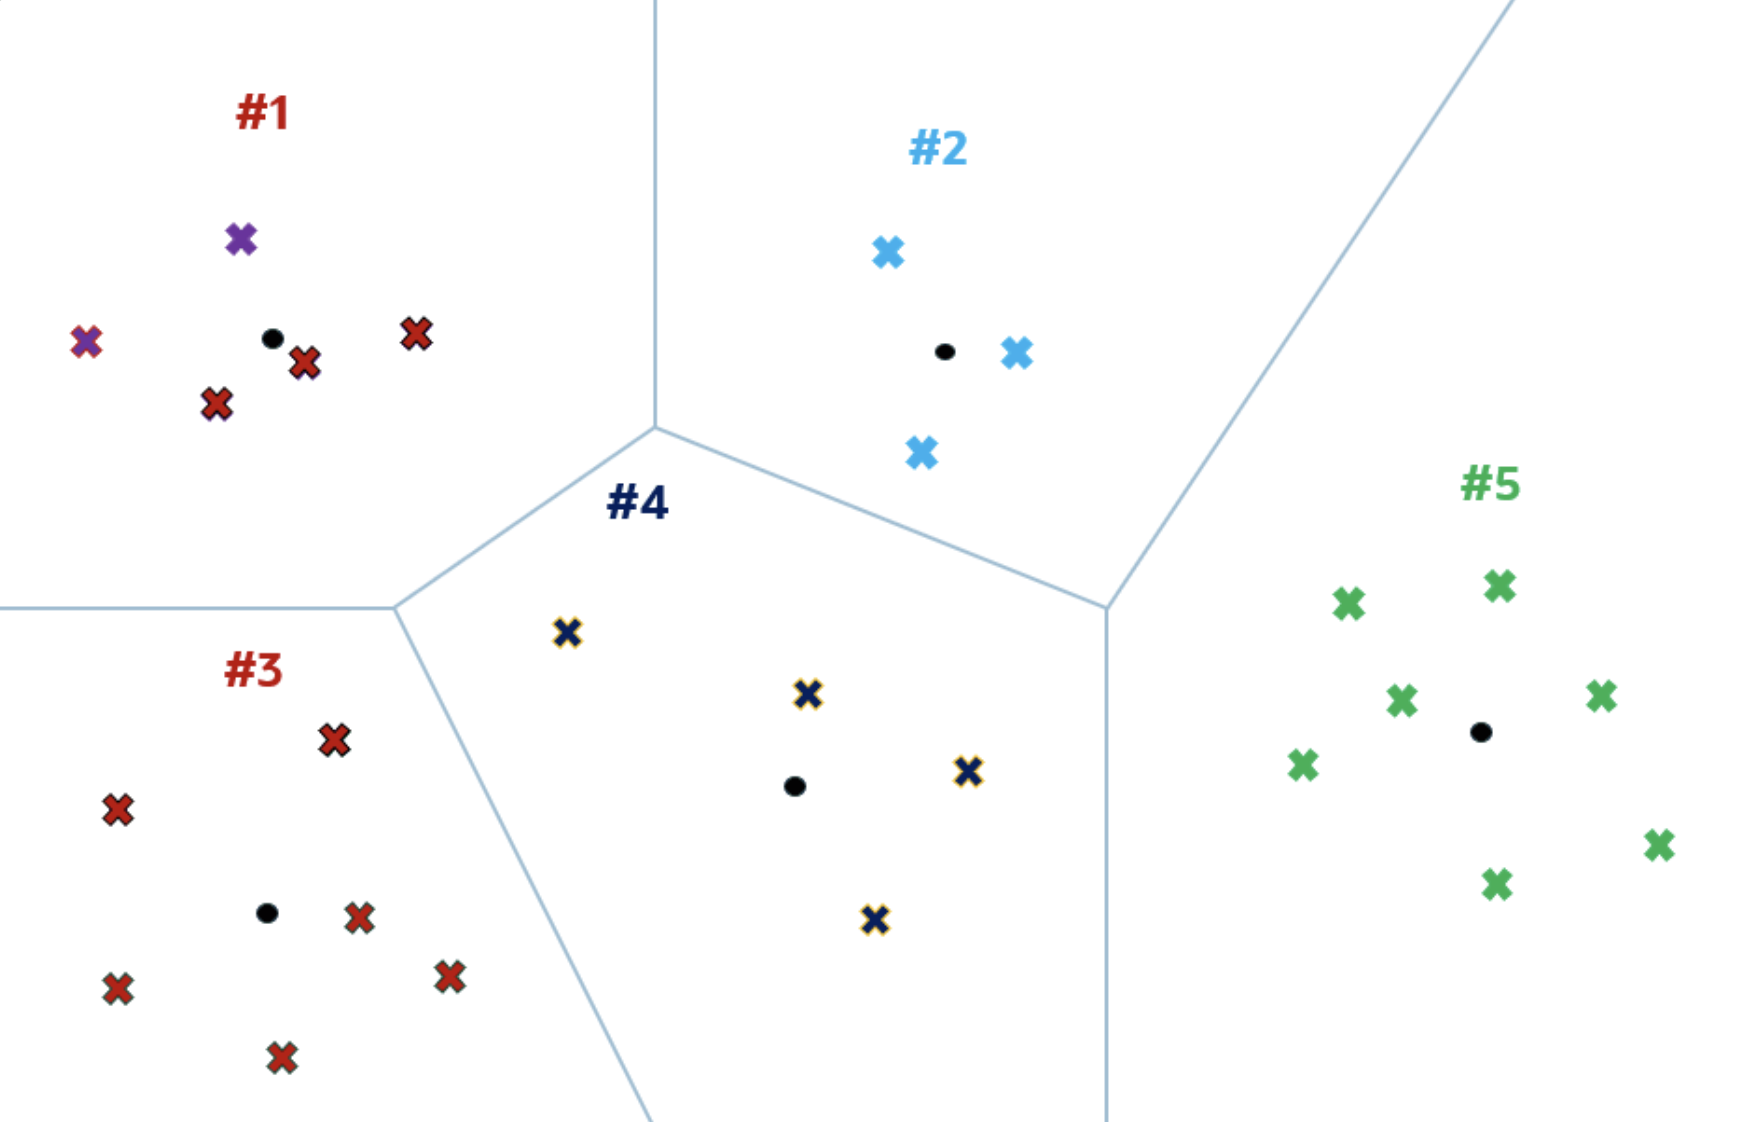
\includegraphics[width=0.72\textwidth]{./assets/voronoi_cells.png}
\caption{Example of a vector space partitioned into Voronoi cells. Each cell is associated with one coarse centroid, and each database vector is assigned to the inverted list of its closest centroid. Adapted from Oracle Database documentation \cite{oracle_ivf_flat}.}
\label{fig:voronoi-cells}
\end{figure}

Search is divided into a coarse quantization stage and a fine-search stage over the selected inverted lists \cite{faiss}. During coarse search, the query is compared with the \(N_{\mathrm{list}}\) centroids. The closest \(N_{\mathrm{probe}}\) centroids are selected. Fine search then evaluates the vectors contained in the corresponding inverted lists:
\begin{equation}
\mathcal{D}_{\mathrm{candidate}}(\mathbf{q})=\bigcup_{j\in P(\mathbf{q})}L_j,
\end{equation}
where \(P(\mathbf{q})\) is the set of lists selected for query \(\mathbf{q}\) and
\begin{equation}
\left|P(\mathbf{q})\right|=N_{\mathrm{probe}}.
\end{equation}
\newline
The main IVF parameters are:
\begin{itemize}
\item \(N_{\mathrm{list}}\), the number of coarse clusters or inverted lists into which the dataset is partitioned;
\item \(N_{\mathrm{probe}}\), the number of inverted lists searched for each query.
\end{itemize}

Increasing \(N_{\mathrm{probe}}\) generally increases recall because a larger portion of the dataset is examined, but it also increases execution time and memory traffic. Increasing \(N_{\mathrm{list}}\) produces smaller clusters and can reduce the number of candidates per probed list, although it makes the coarse-search stage more expensive and may produce load imbalance when cluster sizes are not uniform.

The main source of approximation in IVF is the partition-boundary problem. A vector may be very close to the query while belonging to a Voronoi cell whose centroid was not selected during coarse search. In this case, the vector is excluded from the candidate set before its exact distance from the query is computed.

Figure~\ref{fig:ivf-missed-vector} shows a concrete example of this behavior. The dataset is partitioned into five Voronoi cells, and the query \(\mathbf{q}\) belongs to the red cell. The vectors labeled from \(\#1\) to \(\#5\) are the five exact nearest neighbors of the query. Four of these vectors belong to the selected red cell and are evaluated during fine search. However, vector \(\#2\) lies immediately across the boundary in the neighboring blue cell. Because that cell is not probed, vector \(\#2\) is not included in \(\mathcal{D}_{\mathrm{candidate}}(\mathbf{q})\), even though it belongs to the exact top-\(5\) result.

\begin{figure}[htbp]
\centering
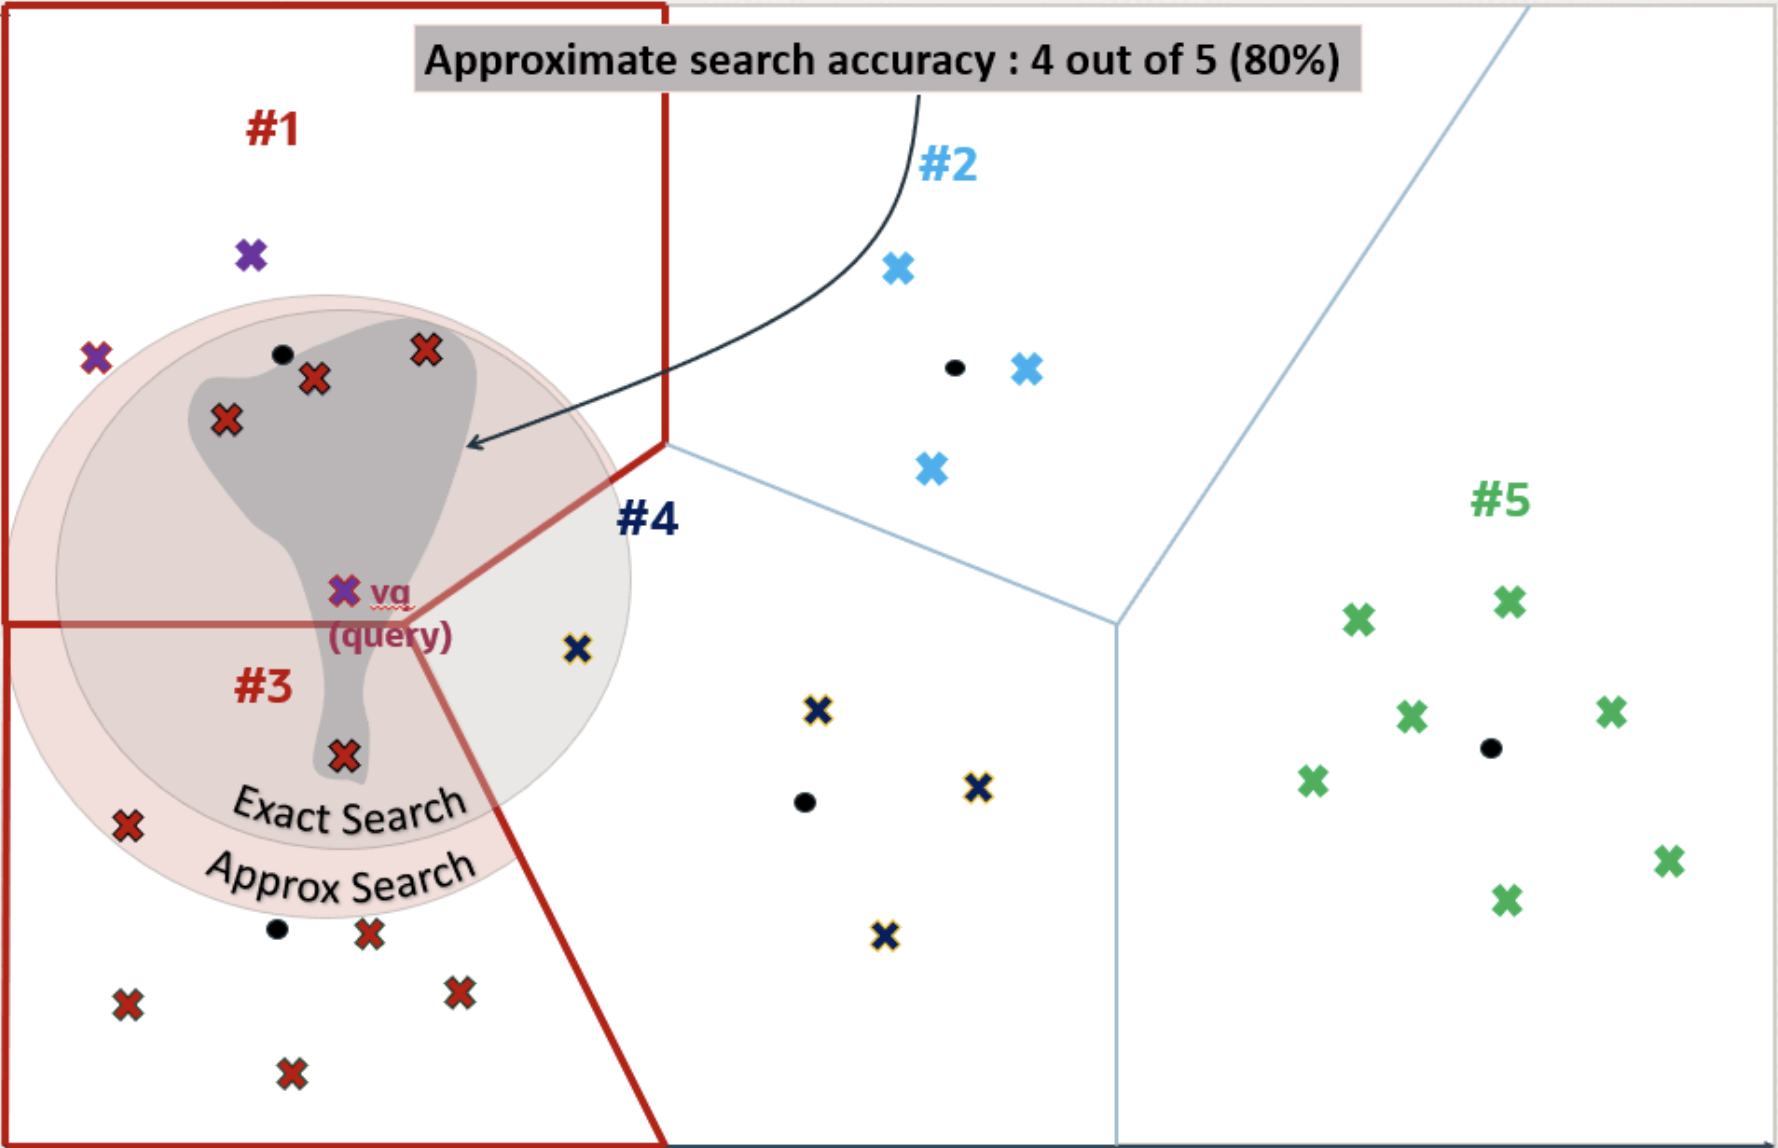
\includegraphics[width=0.95\textwidth]{./assets/ivf_missed_vector.png}
\caption{Example of a missed nearest neighbor in IVF search. The vectors labeled from \(\#1\) to \(\#5\) form the exact top-\(5\) result. Vector \(\#2\) lies in an unprobed neighboring Voronoi cell and is therefore excluded from the approximate result, which retrieves four of the five exact nearest neighbors.}
\label{fig:ivf-missed-vector}
\end{figure}

Using the recall definition introduced in Section~\ref{sec:ann}, the approximate result in Figure~\ref{fig:ivf-missed-vector} achieves
\begin{equation}
\operatorname{Recall@5}=\frac{\left|\operatorname{ANN}_5(\mathbf{q})\cap\operatorname{NN}_5(\mathbf{q})\right|}{5}=\frac{4}{5}=0.8.
\end{equation}

The missed vector is not caused by an inaccurate distance calculation. Its distance is never evaluated because coarse search excludes the inverted list containing it. Increasing \(N_{\mathrm{probe}}\) may include the neighboring blue cell and recover vector \(\#2\), but it also increases the number of candidate vectors, distance computations, and memory transfers.

Despite this limitation, IVF exposes substantial parallelism. Coarse distances can be computed independently, selected clusters can be searched concurrently, and distance computation within each cluster is regular. Vectors in an inverted list can also be stored contiguously, providing more predictable memory accesses than pointer-based index structures.

IVF-Flat stores the original vectors inside each inverted list. Consequently, the distances evaluated during fine search are exact with respect to the selected candidates; approximation is introduced only by the coarse partitioning and the selection of a subset of the lists.

Several extensions reduce the memory footprint or the amount of fine-search work. IVF-PQ stores product-quantized codes instead of complete vectors, while related methods compute approximate distances in the compressed domain \cite{faiss}. ScaNN combines search-space pruning with quantization techniques, including anisotropic vector quantization for maximum inner-product search \cite{scann}. These approaches can significantly reduce memory traffic but introduce additional codebook lookups, approximate-distance computations, and often a re-ranking stage.

\section{Graph-Based Indexes}
\label{sec:graph-indexes}

Graph-based ANN methods represent dataset vectors as vertices of a proximity graph. Edges connect vectors that are close according to the selected metric. At query time, search starts from one or more entry vertices and repeatedly moves toward neighboring vertices that appear closer to the query.

Unlike IVF, graph search does not define a fixed set of spatial partitions to visit. The visited region is determined dynamically by the distances observed during traversal. This can provide high recall while evaluating a relatively small fraction of the dataset, including points located across coarse partition boundaries.

Graph-based methods are particularly effective on CPUs because CPUs provide efficient branch execution, cache hierarchies optimized for irregular access, and SIMD instructions for computing distances between a query and a small set of candidate vectors. Their main disadvantage is that traversal is data-dependent: different queries visit different vertices, perform different numbers of iterations, and access different memory locations.

The two representative graph-based approaches considered in this chapter are HNSW, described in Section~\ref{subsec:hnsw}, and NGT, described in Section~\ref{subsec:ngt}.

\subsection{HNSW: Hierarchical Navigable Small World}
\label{subsec:hnsw}

Hierarchical Navigable Small World, or HNSW, organizes proximity connections into multiple layers \cite{hnsw}. The bottom layer contains all indexed vectors, while progressively higher layers contain increasingly sparse subsets.

The level assigned to each vector is selected probabilistically, with the probability of appearing at higher levels decreasing exponentially. This creates a hierarchy conceptually similar to a skip list: upper layers contain long-range connections that allow the search to move rapidly across the dataset, while lower layers provide increasingly local refinement \cite{skiplist}.

Search begins from an entry point in the highest layer. At each level, the algorithm greedily follows neighbors that improve the distance to the query. Once no closer neighbor is found, the search continues from the current vertex in the next lower layer. At the bottom layer, a wider best-first search is performed using a dynamically maintained candidate queue \cite{hnsw}.
\newline
A simplified representation of the search procedure is:
\begin{enumerate}
\item select an entry vertex in the highest graph layer.
\item greedily traverse the current layer toward the query.
\item use the resulting vertex as the entry point for the layer below.
\item at the bottom layer, maintain a bounded set of promising candidates.
\item terminate when the remaining candidates cannot improve the current result set.
\end{enumerate}

Figure~\ref{fig:hnsw} illustrates this hierarchical organization. The upper layers contain only a sparse subset of the indexed vectors and provide long-range edges that allow the search to move rapidly toward the region containing the query. After reaching a local minimum in one layer, the search descends to the corresponding vertex in the next denser layer. The final and most detailed exploration is performed in layer \(0\), which contains all indexed vectors. This hierarchy allows HNSW to combine coarse navigation in the upper layers with fine-grained neighbor exploration in the bottom layer.

\begin{figure}[htbp]
\centering
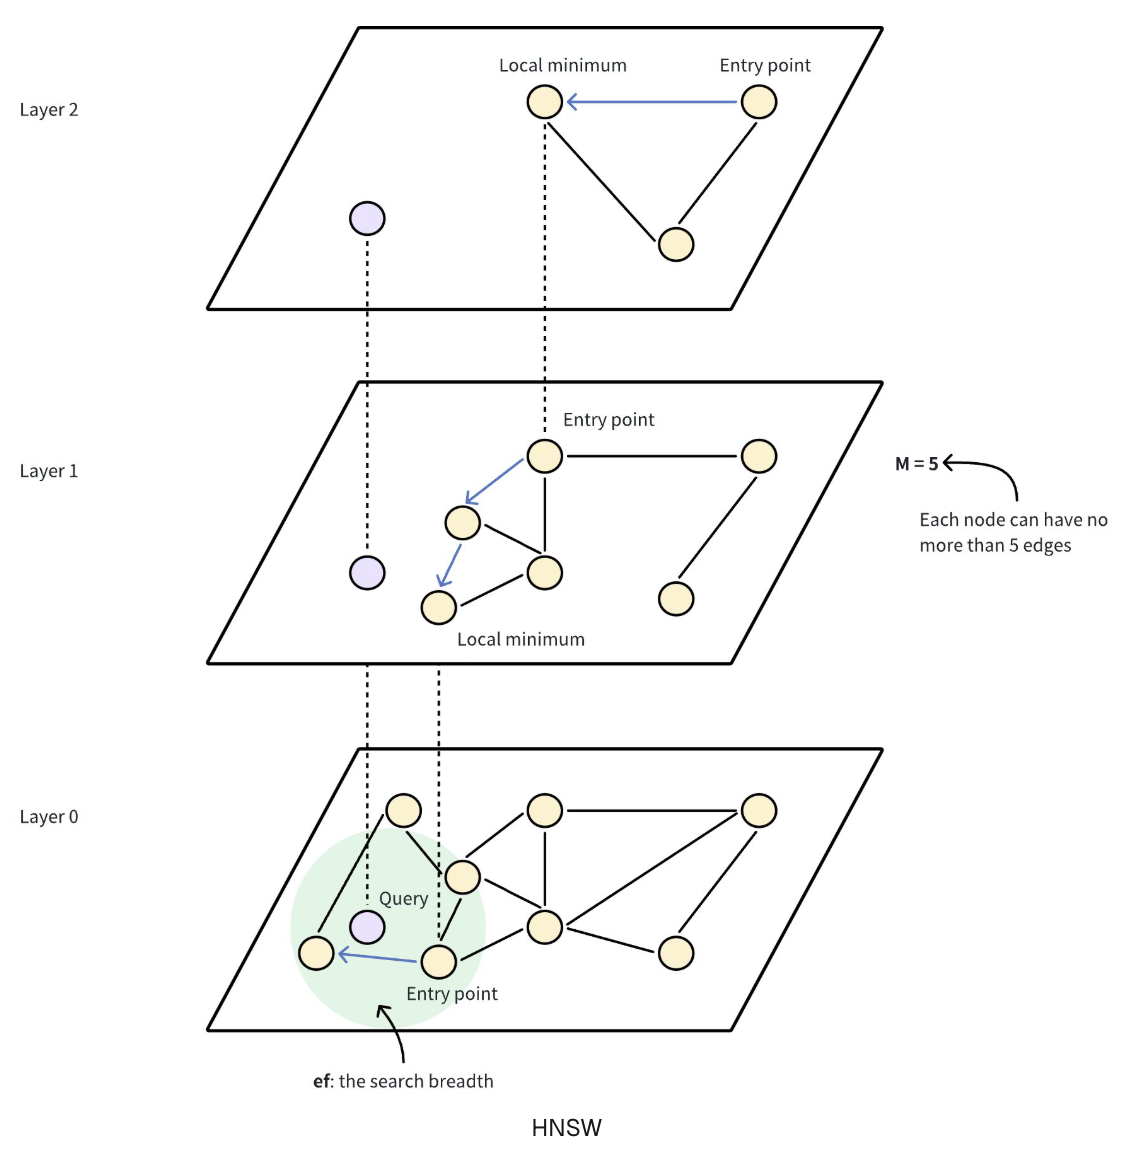
\includegraphics[width=0.78\textwidth]{./assets/hnsw.png}
\caption{Hierarchical organization of an HNSW index. Sparse upper layers provide long-range navigation, while the dense bottom layer supports fine-grained nearest-neighbor search. Adapted from the Milvus HNSW documentation \cite{milvus_hnsw}.}
\label{fig:hnsw}
\end{figure}

The maximum number of connections per vertex and the candidate-list size control the memory, recall, and latency trade-offs. HNSW is known for strong high-recall performance but may require substantial memory because both the original vectors and graph adjacency lists must be stored.
\newline
From an accelerator perspective, HNSW presents several challenges:
\begin{itemize}
\item neighbor addresses depend on the currently visited vertex;
\item adjacency lists and vectors may be distributed across memory;
\item the search frontier and result queue are updated dynamically;
\item different queries follow different paths and terminate after different numbers of steps;
\item visited-set management requires additional random accesses and synchronization.
\end{itemize}

These characteristics do not prevent accelerator implementations, but they make it harder to obtain the regular, high-throughput execution typically associated with dense tensor operations. Unlike the IVF partitioning described in Section~\ref{sec:ivf-background}, HNSW can cross coarse spatial boundaries by traversing graph edges. The consequences of its irregular traversal for Tenstorrent are discussed in Section~\ref{subsec:graph-tt-fit}.

\subsection{NGT: Neighborhood Graph and Tree}
\label{subsec:ngt}

Neighborhood Graph and Tree, or NGT, combines a neighborhood graph with a separate tree-based structure used to obtain good entry points for graph traversal \cite{ngt}. Conceptually, it is similar to HNSW in that both methods first try to move the search toward a promising region of the vector space before performing a more detailed local graph exploration.

The main difference lies in how this initial region is reached. In HNSW, the search uses the hierarchy of the graph itself: it starts from sparse upper layers and progressively descends toward the denser bottom layer. NGT instead uses a separate tree-based structure to locate one or more objects that are expected to be close to the query. These objects are then used as entry vertices for the neighborhood graph.

In this sense, the tree in NGT plays a role similar to the upper layers of HNSW, since both mechanisms reduce the need to begin graph traversal from an arbitrary point. However, the two approaches are structurally different. HNSW integrates coarse navigation and local search into a single hierarchical graph, whereas NGT separates the initial tree-based localization from the subsequent neighborhood-graph traversal.

Once the entry vertices have been identified, NGT explores the neighborhood graph by maintaining a candidate set ordered according to distance from the query. The most promising unexplored candidate is expanded, its neighboring vertices are evaluated, and sufficiently close neighbors are inserted into the candidate set. This process continues until the termination condition is satisfied, after which the best \(k\) objects found during traversal are returned.

Figure~\ref{fig:ngt-overview} summarizes the search process. The tree first performs a coarse localization of the query and selects the initial graph vertices. The neighborhood graph is then explored from these seeds to progressively refine the candidate set and obtain the approximate nearest neighbors.

\begin{figure}[htbp]
\centering
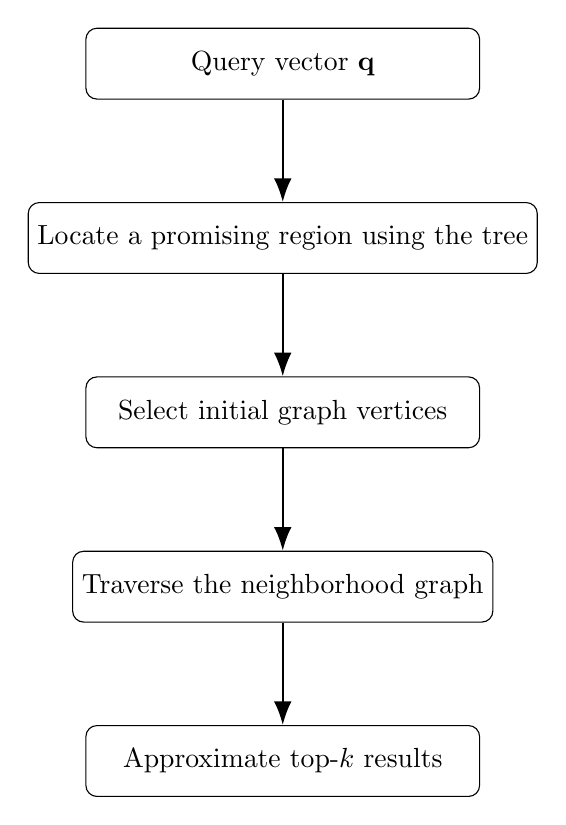
\begin{tikzpicture}[
node distance=1.3cm,
box/.style={draw, rounded corners, minimum width=5.0cm, minimum height=0.9cm, align=center},
arrow/.style={-{Latex[length=3mm]}, thick}
]
\node[box] (query) {Query vector \(\mathbf{q}\)};
\node[box, below=of query] (tree) {Locate a promising region using the tree};
\node[box, below=of tree] (seed) {Select initial graph vertices};
\node[box, below=of seed] (graph) {Traverse the neighborhood graph};
\node[box, below=of graph] (result) {Approximate top-\(k\) results};
\draw[arrow] (query) -- (tree);
\draw[arrow] (tree) -- (seed);
\draw[arrow] (seed) -- (graph);
\draw[arrow] (graph) -- (result);
\end{tikzpicture}
\caption{High-level NGT search process. The tree first identifies a promising region of the vector space and provides initial graph vertices. The neighborhood graph is then explored from these seeds to refine the search and obtain the approximate nearest neighbors. Original illustration based on \cite{ngt}.}
\label{fig:ngt-overview}
\end{figure}

As with HNSW, NGT can achieve high recall while evaluating only a subset of the dataset. Its execution is nevertheless irregular: the next vertices to visit depend on the query and on the distances observed during traversal. The search therefore involves non-contiguous graph accesses, dynamic candidate-set updates, and branch-dependent control flow. The additional tree traversal introduces another query-dependent stage before neighborhood exploration begins.

For this thesis, HNSW and NGT illustrate a common property of graph-based ANN methods: they reduce the number of distance computations by relying on irregular memory accesses and dynamic traversal decisions. These characteristics differ substantially from the regular, tile-oriented execution model targeted by the Tenstorrent architecture, and their suitability is discussed jointly in Section~\ref{subsec:graph-tt-fit}.

\section{GPU-Specialized ANN Indexes}
\label{sec:gpu-indexes}

GPUs provide high arithmetic throughput and memory bandwidth, making them well-suited to regular batched distance computations. However, efficient ANN search on GPUs requires algorithms that expose sufficient parallelism and avoid frequent divergent branches or fine-grained dynamic memory operations.

\subsection{GPU IVF and Faiss}
\label{subsec:gpu-faiss}

IVF naturally maps to GPU execution because many queries, clusters, and candidate vectors can be processed concurrently. GPU implementations can parallelize both the coarse centroid comparisons and the fine-search distance calculations over selected clusters.

One important difficulty is selecting the smallest or largest \(k\) elements from a large set of candidate distances. A conventional heap performs data-dependent insertions and provides insufficient parallelism for efficient GPU execution.

The GPU implementation presented by Johnson et al.\ in Faiss introduces a register-resident selection method designed around GPU warps \cite{faiss}. Candidate values are processed cooperatively by the threads of a warp, reducing global-memory traffic and avoiding the use of a conventional branch-heavy heap. The method is integrated with brute-force, IVF, and product-quantized search.
\newline
The resulting search pipeline uses the GPU effectively because:
\begin{itemize}
\item distance calculations are independent and data parallel;
\item the same kernel can process large batches of queries;
\item candidate vectors can be read through coalesced or block-oriented memory accesses;
\item selection is performed using warp-level cooperation;
\item intermediate results can remain in registers or shared memory.
\end{itemize}

The Faiss work demonstrates that the top-\(k\) stage, rather than only distance computation, must be designed specifically for the target architecture \cite{faiss}.

\subsection{GPU Graph Search and CAGRA}
\label{subsec:cagra}

Traditional proximity-graph indexes are difficult to execute efficiently on GPUs because each query follows a data-dependent path and maintains its own candidate and visited sets. CAGRA addresses this problem through a graph structure and traversal strategy designed specifically for highly parallel GPU execution \cite{cagra}.

CAGRA demonstrates that graph-based ANN search can be adapted to GPUs, but this requires substantially more than transferring a conventional CPU graph traversal to CUDA. Its design modifies both graph construction and query execution to expose bounded and predictable parallel work.

First, CAGRA constructs a single-layer proximity graph with a fixed out-degree, bounding the amount of work associated with each vertex expansion \cite{cagra}. A bounded degree ensures that expanding one graph vertex always produces a known maximum number of neighbors, allowing their vector distances to be evaluated cooperatively by GPU threads. This is considerably more regular than a graph in which adjacency-list lengths vary arbitrarily.

Second, graph traversal is organized around fixed-capacity candidate and result structures rather than dynamically allocated CPU priority queues. Threads within a GPU block cooperate in expanding candidates, computing distances, filtering previously visited vertices, and updating the candidate set. These structures must fit within the memory and synchronization model available to a GPU thread block.

Third, visited-node tracking is implemented using a bounded GPU-oriented structure. Unlike an exact dynamically growing CPU set, this representation accepts limited capacity and possible repeated visits in exchange for predictable memory usage and parallel lookup behavior. The search procedure is therefore designed to tolerate approximation not only in graph traversal but also in auxiliary bookkeeping.

Finally, the stopping policy and the number of expanded candidates are adapted to parallel execution. The algorithm must keep enough work available for the GPU while limiting divergent control flow between queries. These changes show that accelerator graph search requires the graph degree, candidate queue, visited set, work assignment, and termination condition to be co-designed with the target architecture \cite{cagra}.

\subsubsection*{CAGRA versus IVF on GPUs}

Neither CAGRA nor IVF is universally superior on GPUs. The preferable index depends on the required recall, dataset size and distribution, query-batch size, available memory, and index-construction constraints.

IVF exposes regular and highly parallel execution because vectors within each selected inverted list can be read and evaluated in contiguous blocks. Its index structure is comparatively simple, and quantized variants such as IVF-PQ can reduce storage and device-memory bandwidth. However, high-recall search may require probing many inverted lists. As \(N_{\mathrm{probe}}\) increases, the system evaluates more candidate vectors and approaches the cost of exhaustive search.

CAGRA instead uses graph connectivity to navigate toward promising areas of the dataset without scanning entire clusters. Its fixed-degree graph and cooperative GPU traversal are designed to provide high throughput at high recall \cite{cagra}. This advantage comes with additional graph storage, more complex index construction, indirect vector accesses, and candidate and visited-state structures that must be managed during traversal.

CAGRA is therefore particularly attractive for high-recall, memory-resident GPU workloads when graph construction and storage costs are acceptable. IVF remains attractive when regular execution, simpler construction, predictable partitioning, support for datasets larger than available accelerator memory, or compatibility with compression are more important. The comparison is implementation-dependent: optimized quantized IVF variants may outperform graph-based methods at some high-recall operating points \cite{ivf_rabitq_gpu}.

The approach used by CAGRA is highly relevant when considering graph search on Tenstorrent. It shows that accelerator execution is possible, but a direct port of a CPU graph algorithm is unlikely to be efficient. The graph structure, memory layout, candidate management, and traversal strategy must all be redesigned around the target accelerator.

\section{Tenstorrent Architecture and Programming Model}
\label{sec:tt-architecture}

Tenstorrent processors are spatial many-core accelerators whose Tensix cores
form a two-dimensional grid connected through one or more Networks-on-Chip.
Rather than relying primarily on hardware-managed caches and general-purpose
threads, the programming model gives the developer explicit control over data
placement, movement, core assignment, and synchronization.

Figure~\ref{fig:tensix-core} shows the main components of a Tensix core. A core combines local L1 SRAM, RISC-V processors responsible for data movement and kernel control, and specialized compute engines. The data-movement processors issue transfers through the NoC, while the compute path includes a matrix engine for tile-oriented operations and a vector engine for element-wise and special-function operations. The local SRAM stores circular buffers, input and output tiles, intermediate values, runtime metadata, and other kernel state. Consequently, performance depends not only on arithmetic throughput but also on how effectively computation and data movement are pipelined through the limited local-memory capacity.

\begin{figure}[htbp]
\centering
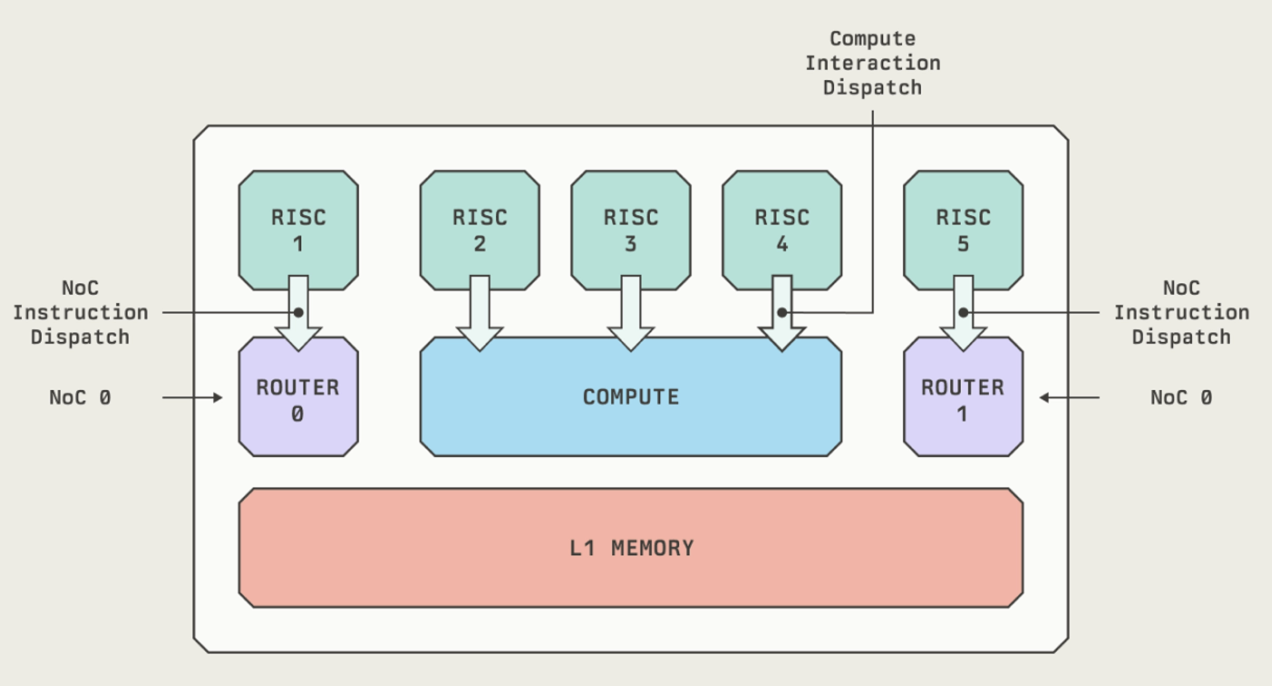
\includegraphics[width=0.82\textwidth]{./assets/tensix.png}
\caption{Simplified organization of a Tensix core, including its RISC-V control and data-movement processors, local L1 SRAM, NoC interfaces, and specialized compute engines. Adapted from the Tenstorrent architecture and TT-Metalium documentation \cite{tenstorrent_metalium_architecture}.}
\label{fig:tensix-core}
\end{figure}

Tenstorrent provides several programming layers with different levels of abstraction. At the highest level considered here, TT-NN provides a Python interface and a library of common tensor and machine-learning operations. It is suitable when an application can be expressed using operations already provided by the library, allowing the runtime to manage much of the device configuration and tensor placement.

TT-Lang provides an intermediate programming layer between TT-NN and TT-Metalium. It is a Python-based domain-specific language for implementing custom Tenstorrent operations while retaining explicit control over data movement, synchronization, and inter-core communication. It provides higher-level constructs such as tensor slices, blocks, and pipes, while remaining more flexible than the predefined operations available in TT-NN. TT-Lang was under active development during this work, and the implementation presented in this thesis was developed directly using TT-Metalium.

TT-Metalium is the lower-level C++ programming interface used to define programs, allocate buffers, select Tensix cores, configure circular buffers, compile kernels, set runtime arguments, and explicitly schedule data movement. TT-Metalium exposes the architecture in sufficient detail to implement non-standard operations such as the ANN kernels developed in this thesis. A typical operation is built from reader, compute, and writer kernels and is first developed for one Tensix core before being distributed across multiple cores or devices.

TT-LLK, or the Low-Level Kernel layer, contains architecture-specific implementations and interfaces for the underlying Tensix compute engines. TT-Metalium compute APIs are commonly built on these lower-level kernels, while direct modification or extension of TT-LLK may be required when the available operations do not expose a needed hardware primitive. In this thesis, the limitations of the available top-\(k\), comparison, and data-manipulation primitives influence which ANN algorithms can be implemented efficiently.

The software stack can therefore be viewed as
\begin{equation}
\text{TT-NN}\rightarrow\text{TT-Lang}\rightarrow\text{TT-Metalium}\rightarrow\text{TT-LLK}\rightarrow\text{Tensix hardware},
\end{equation}
where moving downward provides greater architectural control but also requires more explicit management of memory, synchronization, tilization, and kernel execution.

Most computation on a Tensix core is performed on tiles. The standard tile is a \(32\times32\) block whose elements share the same data type. Tensors whose final dimensions are not multiples of the tile dimensions generally require padding or a different supported layout.
\newline
The relevant memory hierarchy includes:
\begin{itemize}
\item off-chip device DRAM, which provides the capacity required for large tensors and indexes;
\item local L1 SRAM associated with each Tensix core, which provides lower-latency storage for tiles, intermediate values, and circular buffers;
\item explicit transfers over the Network-on-Chip between DRAM interfaces and Tensix cores or among Tensix cores.
\end{itemize}

Data in DRAM is not accessed through a transparent cache. Device kernels explicitly request transfers using the NoC data-movement APIs. Therefore, efficient execution depends strongly on the regularity of the memory-access pattern, the size of each transfer, and the placement of data relative to the cores that consume it.
\newline
A typical TT-Metalium program uses three kinds of kernels:
\begin{itemize}
\item a reader kernel, responsible for transferring input data into local buffers;
\item a compute kernel, which operates on tiles using the Tensix compute engine;
\item a writer kernel, responsible for transferring results to their final location.
\end{itemize}

These kernels communicate through circular buffers in local SRAM. Circular buffers implement a producer--consumer pipeline: a reader reserves space and pushes input tiles, the compute kernel waits for available tiles and produces outputs, and the writer waits for output tiles before transferring them. Double buffering can overlap data movement with computation.
\newline
This execution model is particularly effective for workloads with:
\begin{itemize}
\item regular tile-based computation;
\item statically partitionable work;
\item predictable data movement;
\item contiguous or block-oriented memory accesses;
\item sufficient work per transferred tile;
\item opportunities for batching and data reuse.
\end{itemize}

Conversely, workloads dominated by pointer chasing, fine-grained random access, dynamically sized data structures, and query-dependent control flow are more difficult to map efficiently. Such workloads may still be implementable, but often require transformations that increase the amount of work, memory traffic, or synchronization.

\section{Related Work}
\label{sec:related-work}

\subsection{ANN Search on Specialized Accelerators}

Beyond CPUs and GPUs, ANN search has been mapped to FPGAs, TPUs, and dedicated hardware. FANNS co-designs the parameters of an IVF-PQ index and an FPGA accelerator for a given dataset and recall target, reporting speed-ups of up to 23.0 times over FPGA baselines and 37.2 times over CPU baselines \cite{fanns}. TPU-KNN instead performs nearest-neighbor search on TPUs at close to peak FLOP/s: guided by a performance model that accounts for both memory and instruction bottlenecks, it replaces index traversal with dense matrix computation and outperforms GPU methods at similar recall \cite{tpu_knn}. ANNA proposes a specialized architecture for product-quantization-based ANN search \cite{anna}. TPU-KNN is the closest in spirit to this thesis: both target a matrix-oriented accelerator and trade additional arithmetic for regular, tile-friendly execution.

\subsection{Applications of Tenstorrent Hardware}

Published studies of Tenstorrent hardware beyond machine-learning inference have focused on dense numerical kernels. On the Grayskull e150, a Jacobi stencil reached performance similar to a Xeon Platinum CPU while using about five times less energy \cite{brown_grayskull_stencil}. On the Wormhole, a two-dimensional FFT ran slower than a 24-core Xeon Platinum CPU but consumed about 2.8 times less energy \cite{brown_wormhole_fft}, and a gravitational \(N\)-body simulation on a Wormhole n300 achieved more than a twofold speed-up and about twofold energy savings over an optimized CPU implementation \cite{almerol_wormhole_nbody}.

These workloads have regular, data-independent access patterns. ANN search differs in that the data accessed by each query depends on a data-dependent list selection, list sizes are irregular, and results require a top-\(k\) selection rather than a dense output. To the best of our knowledge, no approximate nearest-neighbor search implementation for Tenstorrent hardware has been published, and this thesis presents the first.

\section{Suitability of ANN Indexes for Tenstorrent}
\label{sec:index-suitability}

The suitability of an ANN index for Tenstorrent depends on more than its algorithmic complexity. An index that performs fewer distance computations may still execute inefficiently if it requires irregular memory accesses, dynamic priority queues, or frequent synchronization.
\newline
The principal criteria considered in this thesis are:
\begin{enumerate}
\item regularity of the computation;
\item spatial locality of the indexed vectors;
\item predictability and granularity of DRAM transfers;
\item ability to batch multiple queries;
\item amount of query-dependent control flow;
\item size and dynamism of intermediate data structures;
\item possibility of statically distributing work across Tensix cores.
\end{enumerate}

\subsection{IVF-Flat}
\label{subsec:ivf-tt-fit}

IVF-Flat provides the most natural mapping among the considered ANN indexes. Both coarse and fine search are dominated by independent vector-distance calculations. The centroids form a dense matrix, while vectors assigned to the same cluster can be stored in contiguous regions of device DRAM.

Coarse search can be performed for a batch of queries by comparing a \(32\)-query tile with tiles containing the centroid vectors. This arrangement matches the native tile dimensions and allows the queries to be reused while centroid blocks are streamed through the compute cores.

Fine search can then be partitioned by assigning selected clusters or groups of clusters to different workers. Each worker reads contiguous vector blocks, computes their distances from the corresponding queries, and produces a local set of candidates. Partial results are subsequently merged.

The implementation developed in this thesis does not treat each query--cluster pair as a completely independent GPU-style task. Instead, work is organized around batches of up to \(32\) queries and the union of the clusters selected for those queries. This allows the data layout and computation to remain compatible with tile-based execution.
\newline
The main difficulties are:
\begin{itemize}
\item inverted lists have different numbers of vectors;
\item different queries may select overlapping or disjoint sets of lists;
\item the amount of work increases with \(N_{\mathrm{probe}}\);
\item workers may receive unequal candidate-set sizes;
\item local candidate sets must be merged into a global top-\(k\);
\item cluster metadata and worker schedules must be generated and transferred efficiently.
\end{itemize}

These issues require explicit scheduling and load balancing, but the dominant computation remains regular enough to benefit from the Tensix architecture. As discussed in Section~\ref{sec:ivf-flat-selection}, this combination of properties made IVF-Flat the index selected for the implementation developed in this thesis.

This section provides only the architectural motivation for mapping IVF-Flat to Tenstorrent. The complete implementation, including the data layout, query batching, coarse-search kernels, fine-search scheduling, top-\(k\) processing, and host--device interaction, is described in Chapter~\ref{chap:design-implementation}.

\subsection{Graph-Based Indexes}
\label{subsec:graph-tt-fit}

Graph-based indexes are less naturally aligned with the current Tenstorrent programming model. To expand one graph vertex, the implementation must first retrieve its adjacency list and then fetch the vectors associated with the listed neighbors. The addresses of these vectors are known only after the current vertex has been processed.

The resulting memory-access sequence is therefore indirect:
\begin{equation}
\text{vertex}\rightarrow\text{adjacency list}\rightarrow\text{neighbor identifiers}\rightarrow\text{neighbor vectors}.
\end{equation}

The neighbor vectors are not guaranteed to be contiguous in DRAM. Transferring complete tiles may consequently fetch vectors that are not needed by the current traversal. Alternatively, issuing small row-major transfers can reduce the transferred volume but may underutilize DRAM and NoC bandwidth.
\newline
Graph traversal also requires:
\begin{itemize}
\item a dynamic candidate queue ordered by distance;
\item a bounded result set;
\item a representation of the previously visited vertices;
\item repeated termination checks;
\item synchronization when multiple workers cooperate on one query.
\end{itemize}

Batching does not completely solve the problem because different queries may visit unrelated regions and execute different numbers of iterations. Some queries may therefore finish while others continue traversing the graph, reducing the utilization of cores assigned to the batch.

Graph indexes should therefore not be described as impossible to implement on Tenstorrent. A possible implementation could use fixed-degree graphs, fixed-capacity candidate buffers, batched frontier expansion, and approximate visited sets. However, this would require a substantial redesign similar in spirit to CAGRA and was beyond the scope of this thesis.

\subsection{CAGRA}
\label{subsec:cagra-tt-fit}

CAGRA is designed for GPU execution, but its GPU-oriented design does not automatically make it efficient on Tenstorrent. Both architectures exploit parallelism, but their execution models and memory hierarchies differ.

The fixed graph degree in CAGRA is beneficial because it bounds the amount of work associated with one vertex expansion. Groups of \(32\) neighbors could, in principle, be arranged to match a Tensix tile dimension. Nevertheless, the identifiers still refer to vectors that may be located in unrelated DRAM regions. Efficiently gathering those vectors remains difficult.

The candidate queue and visited-state structure also require careful consideration. A GPU implementation can use registers, shared memory, and thread-block cooperation to maintain bounded structures. On Tenstorrent, each Tensix core has a limited amount of L1 SRAM that is also used for circular buffers, input tiles, output tiles, metadata, and program state. Reserving a large per-query candidate or visited structure would reduce the space available for double buffering and data reuse.

Placing these structures in device DRAM would increase capacity but introduce additional NoC transfers and latency on every graph iteration. Distributing them over multiple Tensix cores would require synchronization and ownership rules for concurrent updates.
\newline
A Tenstorrent-oriented graph index could still be explored in future work, for example by combining:
\begin{itemize}
\item a fixed graph degree compatible with tile dimensions;
\item batched expansion of several query frontiers;
\item a compact probabilistic visited-state representation;
\item graph reordering to improve spatial locality;
\item bounded iteration counts and fixed-capacity candidate queues.
\end{itemize}

Another possible Tenstorrent-specific design would group multiple dataset vectors into one logical graph vertex. For example, each logical vertex could contain a block of \(32\) vectors, allowing one block to align with a native tile dimension and enabling the distance calculations for those vectors to be performed together. The graph connecting these blocks could use a small fixed degree, such as four outgoing edges. Most edges could connect blocks representing nearby regions, while one edge could provide a longer-range connection intended to improve global navigability.

This organization would reduce the granularity mismatch between conventional graph traversal and tile-oriented execution. Fetching one graph vertex would provide enough vectors to occupy the compute engine, and a fixed low degree would bound the number of successor blocks considered during each expansion. It could also reduce adjacency metadata compared with representing every vector as an independent graph node.

However, grouping vectors changes the semantics of the graph. The \(32\) vectors contained in one block may not all be equally close to one another or to the query, and selecting a block may require evaluating many vectors that would not have been visited by a conventional graph search. Constructing balanced blocks with both good internal locality and useful inter-block edges would therefore become a separate indexing problem. The search would still require a candidate queue, a visited-block representation, query-dependent termination, and indirect DRAM accesses to successor blocks. Long-range edges would also need to be constructed carefully to improve navigability without causing excessive exploration. This design may better match Tensix execution than a conventional per-vector graph, but it does not eliminate the fundamental control-flow and memory-access challenges of graph-based ANN search.

Such an implementation would therefore constitute a separate research project rather than a direct extension of the IVF pipeline.

\subsection{IVF-PQ and Quantized Indexes}
\label{subsec:quantized-tt-fit}

Product quantization \cite{jegou_pq} divides a vector into \(m\) sub-vectors and replaces each sub-vector with the identifier of its closest codeword. A database vector is therefore represented using a short sequence of codebook indices rather than its original coordinates. Figure~\ref{fig:ivf-pq} illustrates this process: the original vector is divided into independent subspaces, each sub-vector is mapped to a codeword from its corresponding codebook, and the resulting codeword identifiers form the compressed representation.

\begin{figure}[htbp]
\centering
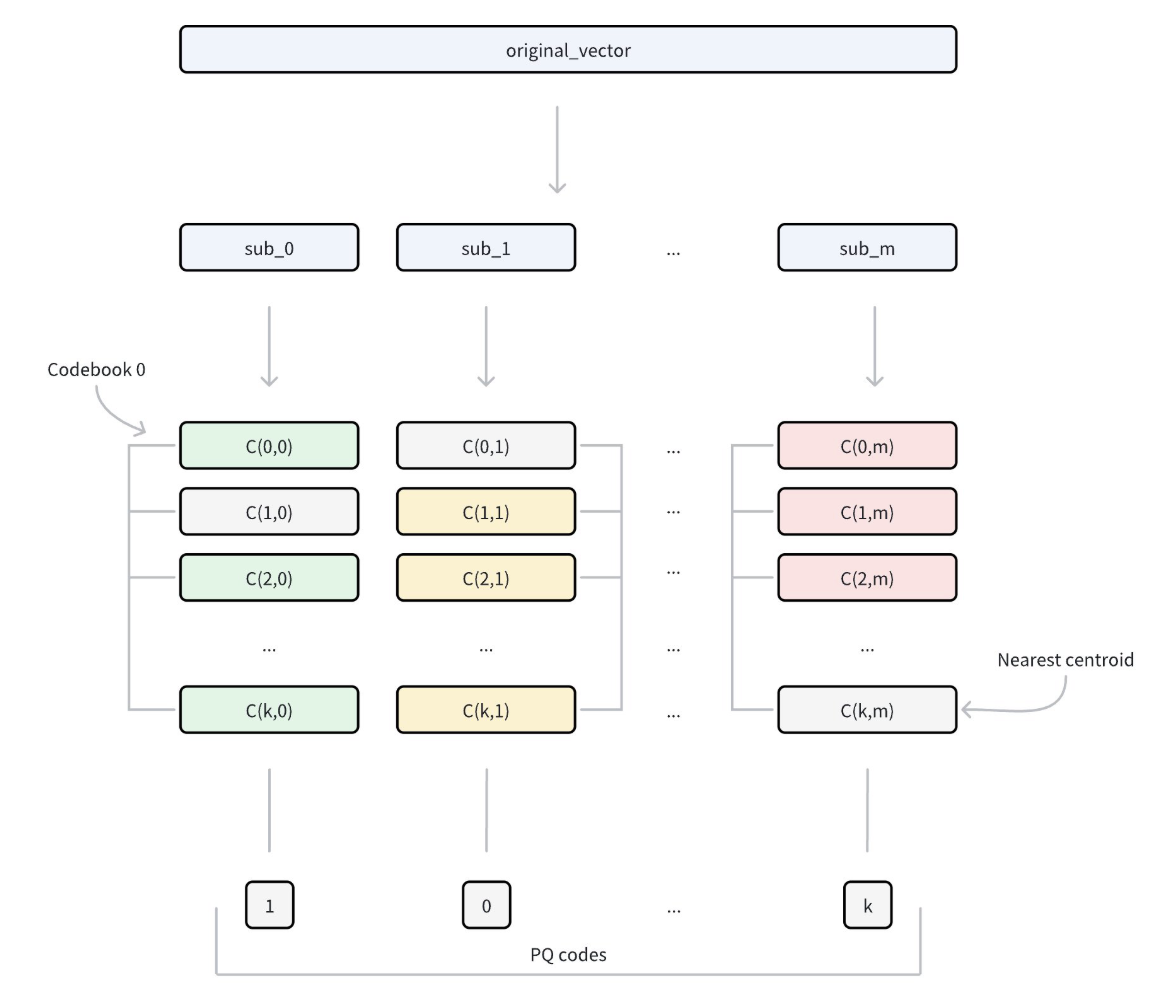
\includegraphics[width=0.82\textwidth]{./assets/ivfpq.png}
\caption{Overview of product quantization within an IVF-PQ index. Each vector is divided into sub-vectors and represented by codeword identifiers from independently trained subspace codebooks. Approximate distances are computed by accumulating values from query-specific lookup tables. Adapted from the Milvus IVF-PQ documentation \cite{milvus_ivfpq}.}
\label{fig:ivf-pq}
\end{figure}

For a query, lookup tables containing the distance between each query sub-vector and each codeword can be precomputed. As shown in Figure~\ref{fig:ivf-pq}, the approximate distance to a compressed database vector is obtained by using its codeword identifiers to select one value from each lookup table and summing the selected values.
\newline
IVF-PQ preserves the coarse partitioning of IVF and therefore retains many of its favorable properties:
\begin{itemize}
\item encoded vectors can be stored contiguously within each inverted list;
\item many codes can be evaluated independently;
\item the reduced representation lowers DRAM capacity and bandwidth requirements;
\item coarse search and cluster scheduling can reuse the IVF-Flat design.
\end{itemize}

The difficulty is not that the original vector must be fetched for every candidate. During the approximate stage, distances can be computed directly from the compressed codes. Original vectors are required only when an optional exact re-ranking stage is performed.
\newline
The main implementation challenges on Tenstorrent are:
\begin{itemize}
\item implementing efficient small-table lookups;
\item decoding packed codeword identifiers;
\item supporting integer and mixed-precision accumulation;
\item arranging codebooks for efficient local reuse;
\item gathering original vectors if exact re-ranking is enabled.
\end{itemize}

Although IVF-PQ reduces the amount of data stored in DRAM, its fine-search access pattern is less suitable for the current Tenstorrent implementation than the sequential reading of full vectors used by IVF-Flat. Each candidate code contains several packed codeword identifiers, and evaluating it requires decoding those identifiers and performing multiple indexed accesses into relatively small distance tables. These gathers are regular at the algorithmic level but do not directly correspond to the dense tile operations for which the available Tensix compute primitives are optimized.

The lookup tables could be copied into local SRAM and reused across many candidates, but each Tensix core would then need sufficient local capacity for the tables, circular buffers, candidate codes, intermediate distances, and top-\(k\) state. If the tables or decoded data cannot remain local, repeated accesses through device memory or the NoC may offset part of the bandwidth reduction obtained from compression. Packed-code extraction and mixed-precision accumulation would also require additional low-level kernels.

For these reasons, IVF-PQ was not considered a promising first index for the current implementation. This conclusion concerns its mapping to the present Tenstorrent software stack rather than the general efficiency of IVF-PQ. A specialized implementation with local lookup-table reuse, efficient packed-code decoding, and dedicated quantized-distance kernels could make IVF-PQ attractive in future work.

\subsection{ScaNN}
\label{subsec:scann-tt-fit}

ScaNN combines partitioning, quantization, and re-ranking. Its anisotropic quantization objective gives greater importance to preserving components of the quantization residual that have a larger effect on the inner product \cite{scann}.
\newline
A typical ScaNN-style search pipeline combines partition-based pruning, compressed candidate scoring, candidate selection, and optional exact re-ranking \cite{scann}:
\begin{enumerate}
\item partition-based pruning of the search space;
\item approximate scoring of a comparatively large candidate set using highly compressed representations;
\item selection of a sufficiently large set of promising candidates;
\item re-ranking of those candidates using their original vectors to obtain the final top-\(k\) results.
\end{enumerate}

The partitioning and approximate-scoring stages offer parallelism and could potentially be mapped to Tensix cores. However, an efficient implementation would require optimized quantized-distance kernels and a sufficiently large intermediate candidate selection.

In the implementation considered in this thesis, the available top-\(k\) primitive from TT-LLK and the local-memory budget constrain the number of candidates that can be maintained efficiently inside one device program. Re-ranking also requires gathering original vectors whose identifiers were produced by the compressed search stage. Unless the dataset is reordered or the selected identifiers exhibit locality, these vectors may be distributed across device DRAM.

These issues do not make ScaNN fundamentally incompatible with Tenstorrent. They indicate that an efficient implementation would require additional support for large candidate selection, quantized lookups, and batched vector gathering. For this reason, ScaNN was considered beyond the scope of the first Tenstorrent ANN implementation.

\section{Motivation for Selecting IVF-Flat}
\label{sec:ivf-flat-selection}

Section~\ref{sec:index-suitability} compared IVF-Flat, graph-based indexes, CAGRA, IVF-PQ, and ScaNN against the same set of criteria: regularity of computation, spatial locality, DRAM-transfer granularity, batchability, query-dependent control flow, and the possibility of static work distribution. IVF-Flat was the only index for which all of these criteria were favorable without requiring a substantial architectural redesign, which is why it was selected for the implementation developed in this thesis.

Two further points reinforced this choice. First, IVF-Flat avoids compression-related approximation during candidate scoring: once a list has been selected, its vectors are compared with the query using their original representation. This simplifies correctness validation and allows the effects of \(N_{\mathrm{list}}\), \(N_{\mathrm{probe}}\), scheduling, and data movement to be studied directly without conflating them with quantization error.

Second, IVF still exposes challenges representative of real accelerator systems, including variable cluster sizes, load balancing, host-side scheduling, DRAM placement, NoC traffic, local top-\(k\) selection, and result merging, without requiring the fully dynamic execution model of graph-based search.

Table~\ref{tab:ann-index-summary} summarizes the principal trade-offs of the index families considered in this chapter.

\begin{table}[htbp]
\centering
\caption{Summary of the ANN indexes considered and their qualitative suitability for the current Tenstorrent programming model.}
\label{tab:ann-index-summary}
\small
\setlength{\tabcolsep}{4pt}
\renewcommand{\arraystretch}{1.15}
\begin{tabular}{p{1.6cm}p{2.5cm}p{2.7cm}p{3.7cm}}
\toprule
Index & Main advantage & Main limitation & Tenstorrent suitability \\
\midrule
Flat & Regular exhaustive computation & Linear work in dataset size & Regular, but excessively expensive at scale \\
IVF-Flat & Contiguous candidate scans and tunable recall & May miss vectors in unprobed cells & High; selected for this thesis \\
HNSW & High recall with relatively few distance evaluations & Irregular traversal and substantial graph state & Low without substantial redesign \\
NGT & Tree-based seeding followed by graph refinement & Dynamic traversal and indirect memory accesses & Low without substantial redesign \\
CAGRA & GPU-oriented high-recall graph search & Complex traversal state and indirect accesses & Potentially feasible with a TT-specific redesign \\
IVF-PQ & Reduced storage and memory traffic & Packed decoding and lookup-table accesses & Moderate, but difficult with current primitives \\
ScaNN & Effective pruning, quantization, and re-ranking & Large intermediate selection and irregular re-ranking & Moderate to low with the current software stack \\
\bottomrule
\end{tabular}
\end{table}

The selection of IVF-Flat should not be interpreted as evidence that other ANN indexes cannot execute on Tenstorrent. Instead, IVF-Flat is the index whose computation, memory layout, and scheduling requirements most directly match the capabilities of the current architecture and software stack. It provides a suitable starting point for studying the feasibility, performance, energy efficiency, and bottlenecks of ANN search on Tenstorrent hardware. Its complete implementation is presented in Chapter~\ref{chap:design-implementation}.

\cleardoublepage


\chapter{Design and Implementation}
\label{chap:design-implementation}

\section{System Architecture}
\label{sec:system-architecture}
This chapter presents the system design and implementation of a Tenstorrent-oriented IVF-Flat approximate nearest-neighbour search pipeline on a single-chip Tenstorrent Wormhole n150 device using TT-Metalium \cite{tenstorrent_metalium_architecture,tenstorrent_wormhole_spec}. IVF-Flat provides the underlying indexing algorithm; the contribution of this chapter is its mapping to the target accelerator. In particular, the design maps regular, fixed-shape operations, including centroid scoring and page-wise candidate scoring, onto the tile-oriented Tensix execution model, while explicitly handling the irregularity caused by query-dependent list selection and unequal inverted-list sizes. The architectural meaning of regular and irregular execution is introduced in Section~\ref{sec:index-suitability}.

The implementation is organised around two principal device programs: a \emph{coarse-search program}, which compares queries with the IVF centroids, and a \emph{fine-search program}, which evaluates candidate vectors from the selected inverted lists and reduces the results to the final top-\(k\). Host-side processing connects the two phases by selecting the \(N_{\mathrm{probe}}\) lists returned by coarse search and constructing the work schedule used by the fine-search workers.

\subsection{End-to-End Search Pipeline}
\label{subsec:end-to-end-pipeline}

A query is first compared with all \(N_{\mathrm{list}}\) centroids, after which the \(N_{\mathrm{probe}}\) most similar centroids identify the inverted lists to be searched. Candidate vectors contained in those lists are then compared with the query, and the final top-\(k\) scores and vector identifiers are selected from the resulting similarities. This logical IVF-Flat pipeline is summarised in Figure~\ref{fig:ivf-search-pipeline}.

\begin{figure}[htbp]
\centering
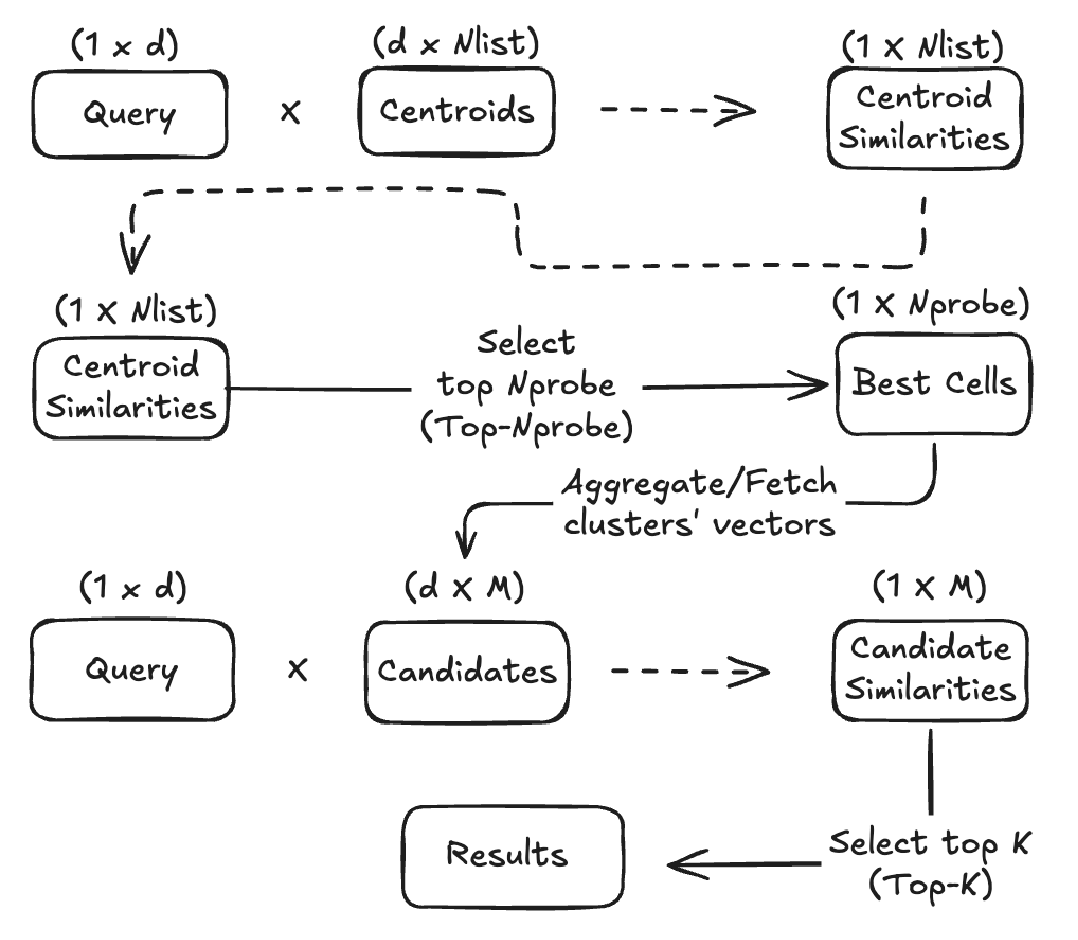
\includegraphics[width=0.90\textwidth]{./assets/ivf_search_pipeline.png}
\caption{Logical IVF-Flat query-processing pipeline. The query is first compared with all \(N_{\mathrm{list}}\) centroids. The \(N_{\mathrm{probe}}\) best cells are selected, their vectors define the candidate set, and the final top-\(k\) results are selected from the candidate similarities.}
\label{fig:ivf-search-pipeline}
\end{figure}

The figure is intentionally logical rather than physical: selected candidates are not copied into a single temporary matrix. Instead, database vectors remain grouped by inverted list in device memory and are streamed directly from the selected complete lists during fine search.

Queries are represented internally in groups containing between one and 32 valid queries, matching the row dimension of the \(32\times32\) tile representation used by the Tensix compute kernels. A group containing fewer than 32 valid queries is completed with zero-valued padded rows. For a workload containing \(Q\) valid queries, the implementation uses
\begin{equation}
B=\left\lceil\frac{Q}{32}\right\rceil
\end{equation}
internal query batches. The final batch is padded when \(Q\) is not divisible by 32. The number of valid rows is retained separately, so padded rows do not participate in coarse-result processing and do not contribute inverted lists to the fine-search schedule. They are also discarded when the final results are converted back to the host representation.

Although the implementation is described throughout the chapter in terms of one 32-query batch for clarity, the final system can process multiple such batches within one coarse-search and one fine-search invocation. The transition from the initial single-batch implementation to this multi-batch design is discussed in Section~\ref{sec:multi-batch-execution}.

\subsection{Host--Device Work Partitioning}
\label{subsec:host-device-responsibilities}

The index data required by both search stages remain resident on the Tenstorrent device across query workloads, including the centroid matrix, database vectors grouped by inverted list, and the corresponding original vector identifiers. In contrast, query-dependent data, such as the query buffer, coarse-search outputs, selected-list metadata, worker schedules, partial results, and final outputs, are updated for each search workload.

A synchronization boundary separates the coarse and fine programs. After the device executes coarse search and returns a fixed-size set of centroid candidates for each valid query, the host performs the final \(N_{\mathrm{probe}}\) selection, obtains the offset and padded length of each corresponding complete inverted list, groups the selected work at batch granularity, and constructs the per-worker fine-search descriptions. Only once this query-dependent schedule has been prepared is the fine-search program launched.

Figure~\ref{fig:host-device-pipeline} shows the division of responsibilities between the host and the device, together with the synchronization boundary between coarse and fine search.

\begin{figure}[htbp]
\centering
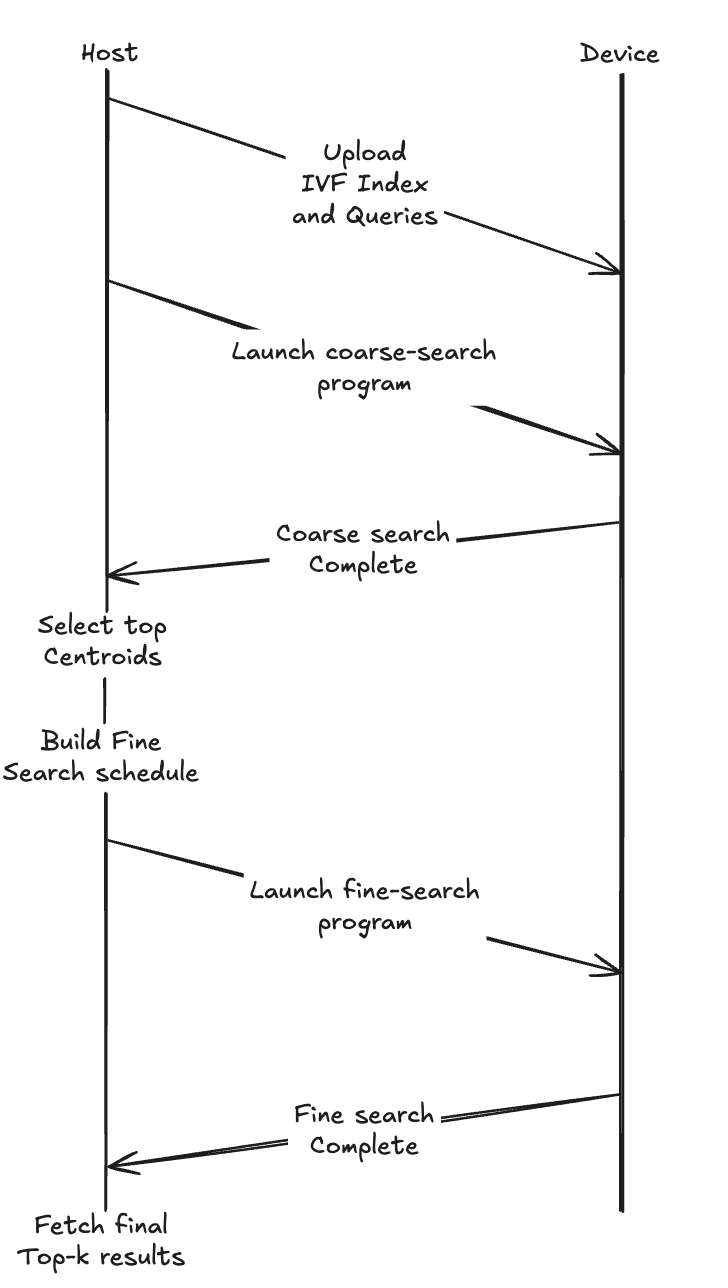
\includegraphics[width=0.80\textwidth]{./assets/host_device_pipeline.png}
\caption{Host--device interaction during one IVF search workload. The host loads the IVF index and query batch, launches the coarse-search program, receives the coarse-search results, selects the \(N_{\mathrm{probe}}\) lists and builds the fine-search schedule, then launches the fine-search program and fetches the final top-\(k\) results.}
\label{fig:host-device-pipeline}
\end{figure}

Each device program is decomposed into \emph{reader}, \emph{compute}, and \emph{writer} kernels connected through circular buffers, allowing data movement and computation to overlap when dependencies and buffer capacity permit it. Throughout this chapter, reader, compute, and writer denote kernels executing on a Tensix core, whereas worker and aggregation core denote logical roles assigned to complete Tensix cores. The terms \emph{coarse phase} and \emph{fine phase} refer to complete TT-Metalium programs rather than to individual kernels.

\section{Device-Oriented IVF Representation}
\label{sec:device-oriented-ivf}

\subsection{Index Construction}
\label{subsec:index-construction}

Index training is treated as an offline preprocessing step and is outside the timed search path. A representative subset of the database vectors is clustered with Faiss \(k\)-means to obtain \(N_{\mathrm{list}}\) centroids \cite{faiss}, following the same training procedure used by the CPU and GPU baselines based on Faiss \texttt{IndexIVFFlat}. The trained centroid matrix is exported and reused by the Tenstorrent implementation. Reusing the same centroids avoids making index-training quality an additional experimental variable and allows the evaluation to focus on differences in search execution.

Training is not performed on the Tenstorrent device because the objective of this work is the online IVF search path rather than accelerator-based \(k\)-means. An on-device training implementation would require additional iterative kernels for vector assignment, per-cluster accumulation, centroid normalisation, and convergence control, together with temporary device-memory capacity for the intermediate state. Those operations would neither be part of the measured query path nor improve the fairness of the search comparison. During construction of the Tenstorrent-oriented index, each database vector is assigned to its closest exported centroid and placed in the corresponding packed inverted list.

The Tenstorrent index stores full, uncompressed database vectors rather than compressed representations. Database vectors and centroids are normalised before assignment and search, allowing inner product to be used as the similarity measure.

Because the resulting inverted lists are not guaranteed to have equal sizes, assigning the same number of lists to every core does not necessarily assign the same amount of work. The fine-search scheduler therefore reasons about the number of 32-vector pages contained in each selected list rather than only the number of lists.

\subsection{Tiled Data Layout and Memory Placement}
\label{subsec:tiled-list-layout}

As introduced in Chapter~\ref{chap:background}, Tensix computation is organised around \(32\times32\) tiles \cite{tenstorrent_metalium_architecture}. Let \(D\) denote the original vector dimension. To match this tile-oriented execution model, the dimension is padded to
\begin{equation}
D_{\mathrm{p}}=32\left\lceil\frac{D}{32}\right\rceil.
\label{eq:dimension-padding}
\end{equation}
All values introduced by dimensional padding are set to zero on the host before the data are transferred to the device.

Vectors assigned to the same inverted list are stored consecutively in one logical packed database buffer. For a list containing \(L_j\) valid vectors, its stored length is rounded to a multiple of 32:
\begin{equation}
L_{j,\mathrm{p}}=32\left\lceil\frac{L_j}{32}\right\rceil.
\label{eq:list-padding}
\end{equation}
Each group of 32 vectors forms one \emph{candidate page}. A page contains \(D_{\mathrm{p}}/32\) 16-bit floating-point (\texttt{FP16}) data tiles, each of shape \(32\times32\), which together represent the 32 candidate vectors over the complete padded dimension. Centroids and queries use the same \texttt{FP16} representation, while vector identifiers are stored as 32-bit unsigned integers (\texttt{UInt32}). The Tenstorrent compute configuration enables FP32 destination accumulation. This mode is required by the employed top-\(k\) path when score tiles are ordered together with \texttt{UInt32} identifier tiles.

A candidate page must not be confused with a query batch. A query batch contains up to 32 queries and forms the row operand of fine search, whereas a candidate page contains 32 database vectors and forms the column operand. Their matrix product evaluates every query in the batch against every vector in the page. Figure~\ref{fig:pedagogical-batch-page} illustrates this distinction with a \(4\times4\) example.

\begin{figure}[htbp]
\centering
\resizebox{0.98\textwidth}{!}{%
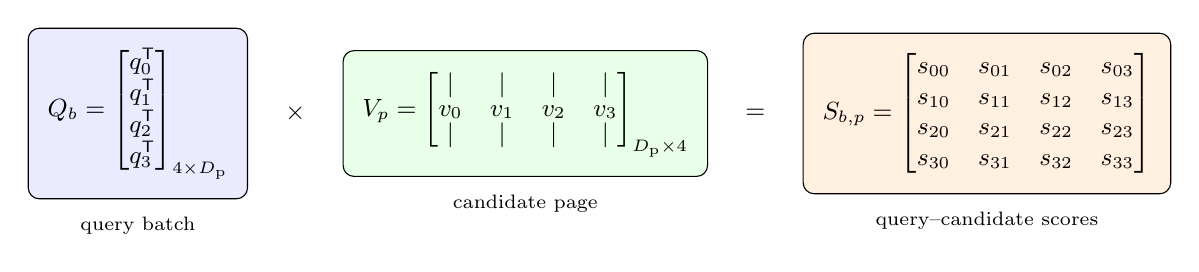
\begin{tikzpicture}[font=\small]
\node[draw,rounded corners,fill=blue!8,inner sep=7pt] (queries) {$
Q_b=
\begin{bmatrix}
q_0^{\mathsf T}\\
q_1^{\mathsf T}\\
q_2^{\mathsf T}\\
q_3^{\mathsf T}
\end{bmatrix}_{4\times D_{\mathrm p}}
$};
\node[draw,rounded corners,fill=green!9,inner sep=7pt,
      right=1.2cm of queries] (page) {$
V_p=
\begin{bmatrix}
\vert&\vert&\vert&\vert\\[-2pt]
v_0&v_1&v_2&v_3\\[-2pt]
\vert&\vert&\vert&\vert
\end{bmatrix}_{D_{\mathrm p}\times4}
$};
\node[draw,rounded corners,fill=orange!12,inner sep=7pt,
      right=1.2cm of page] (scores) {$
S_{b,p}=
\begin{bmatrix}
s_{00}&s_{01}&s_{02}&s_{03}\\
s_{10}&s_{11}&s_{12}&s_{13}\\
s_{20}&s_{21}&s_{22}&s_{23}\\
s_{30}&s_{31}&s_{32}&s_{33}
\end{bmatrix}
$};
\node at ($(queries.east)!0.5!(page.west)$) {$\times$};
\node at ($(page.east)!0.5!(scores.west)$) {$=$};
\node[below=3pt of queries,font=\scriptsize] {query batch};
\node[below=3pt of page,font=\scriptsize] {candidate page};
\node[below=3pt of scores,font=\scriptsize] {query--candidate scores};
\end{tikzpicture}
}
\caption{Pedagogical \(4\times4\) example of one fine-search matrix
multiplication. Rows represent queries and columns represent candidate vectors.
The implementation uses \(32\times32\) tiles rather than the reduced size
shown here.}
\label{fig:pedagogical-batch-page}
\end{figure}

For every candidate page, one full \(32\times32\) \texttt{UInt32} identifier tile is stored. In its DRAM representation, each column corresponds to one candidate vector and the same 32 identifiers are replicated across all query rows. For candidate identifiers \(i_0,\ldots,i_{31}\), the stored tile is
\begin{equation}
I^{\mathrm{stored}}=
\begin{bmatrix}
i_0 & i_1 & \cdots & i_{31}\\
i_0 & i_1 & \cdots & i_{31}\\
\vdots & \vdots & \ddots & \vdots\\
i_0 & i_1 & \cdots & i_{31}
\end{bmatrix}.
\label{eq:identifier-tile}
\end{equation}
Before the compute-kernel \texttt{topk\_local\_sort} operation, both the similarity tile and its companion identifier tile are transposed. The identifier tile presented to the selection operation is therefore
\begin{equation}
I^{\mathrm{topk}}
=
\left(I^{\mathrm{stored}}\right)^{\mathsf T}
=
\begin{bmatrix}
i_0 & i_0 & \cdots & i_0\\
i_1 & i_1 & \cdots & i_1\\
\vdots & \vdots & \ddots & \vdots\\
i_{31} & i_{31} & \cdots & i_{31}
\end{bmatrix}.
\label{eq:identifier-tile-topk}
\end{equation}
After transposition, each column corresponds to one query and the rows represent candidate entries. The \texttt{topk\_local\_sort} operation sorts candidate entries independently for each query column. Applying the same transpose and ordering operations to the score and identifier tiles preserves the association between every similarity value and its original database-vector identifier. This transpose-and-sort mechanism is used by both coarse and fine search whenever a running top-32 score and identifier state is updated.

The vectors of all inverted lists are stored sequentially in a single packed device buffer. Each inverted list is identified by its offset within this buffer and by its length, rather than being stored in a separate device allocation. Vector identifiers occupy a separate packed \texttt{UInt32} buffer using the same list and page ordering. An inverted-list offset therefore identifies a position in this global logical representation. At the physical memory level, TT-Metalium interleaves buffer pages across DRAM banks, so ``contiguous'' refers to the logical buffer layout rather than to consecutive bytes within one DRAM bank.

Persistent search data are allocated in device DRAM, including the centroid matrix, packed database-vector buffer, and packed vector-identifier buffer. Query buffers and worker descriptions are likewise allocated in DRAM for each search workload, while per-core L1 memory is used as transient kernel-local storage through circular buffers. During execution, data required by the active kernels are streamed from DRAM into L1 rather than persistently cached across search invocations. The exact reuse and streaming strategy of the coarse- and fine-search programs is described in Sections~\ref{sec:coarse-search} and~\ref{subsec:fine-worker-pipeline}, respectively.
\newline
Padding is performed entirely on the host before device transfer:
\begin{itemize}
    \item database dimensional padding and inverted-list length padding are generated during \texttt{IVF\_TT::create\_index}.
    \item centroid dimensional padding is generated while constructing the centroid buffer in \texttt{load\_to\_device}.
    \item query dimensional padding and final-batch row padding are generated in \texttt{search\_all}.
\end{itemize}
Padded vector identifiers are assigned the sentinel value \texttt{0xffffffff} on the host.

Padded candidate positions contain zero-valued vectors and carry the sentinel identifiers defined above. Before local top-\(k\) selection, the fine-search compute kernel linearly scans the score and identifier entries of the final partially populated page of each inverted list. Whenever a sentinel identifier is encountered, the corresponding similarity value is replaced with \(-10000\), preventing padded candidates from displacing valid results during selection. The database and query vectors are normalised, so a valid inner product is bounded below by \(-1\) in exact arithmetic; \(-10000\) is therefore safely outside the valid similarity range. Complete candidate pages contain 32 valid vectors and bypass this masking step, avoiding an unnecessary scan of all \(32\times32=1024\) entries when no padding is present.

\section{Coarse Search}
\label{sec:coarse-search}

The purpose of coarse search is to identify the inverted lists most relevant to each query. For a valid query batch \(Q_b\in\mathbb{R}^{32\times D_{\mathrm{p}}}\) and centroid matrix \(C\in\mathbb{R}^{D_{\mathrm{p}}\times N_{\mathrm{list}}}\), the logical operation is
\begin{equation}
S^{\mathrm{coarse}}_b=Q_bC,
\label{eq:coarse-search}
\end{equation}
where each row of \(S^{\mathrm{coarse}}_b\) contains the similarities between one query and all centroids.

Tiling proceeds over blocks of 32 centroids. After loading the query batch from DRAM into an L1 circular buffer, the reader kernel streams centroid blocks from device DRAM while retaining the query for reuse across the complete centroid matrix. Let \(C_c\in\mathbb{R}^{D_{\mathrm{p}}\times32}\) denote centroid block \(c\).

The corresponding coarse-similarity tile is
\begin{equation}
S^{\mathrm{coarse}}_{b,c}=Q_bC_c,
\qquad
S^{\mathrm{coarse}}_{b,c}\in\mathbb{R}^{32\times32}.
\label{eq:coarse-similarity-tile}
\end{equation}
Rather than materialising all \(N_{\mathrm{list}}\) similarities in DRAM, the compute kernel incrementally maintains the 32 highest centroid scores and their identifiers for each query row. This running top-32 state uses the same transpose-and-\texttt{topk\_local\_sort} mechanism described in Section~\ref{subsec:tiled-list-layout}, with identical ordering decisions applied to scores and centroid identifiers.

Once all centroid blocks assigned to a query batch have been processed, the coarse-search writer kernel running on the same participating Tensix core writes one score tile and one identifier tile for that batch to device DRAM. After copying these results to the host, the host orders and deduplicates the valid centroid identifiers and retains the first \(N_{\mathrm{probe}}\) lists for each query. Consequently, the current implementation limits \(N_{\mathrm{probe}}\) to at most 32.

Multiple query batches are distributed by the coarse-search program across the available participating cores, with each active core processing one or more complete batches and avoiding inter-core communication during the centroid scan. Because every valid query is evaluated against the same centroid matrix, coarse search remains regular and requires a predictable amount of work.

\section{Fine-Search Scheduling}
\label{sec:fine-search-scheduling}

Fine search introduces the principal source of irregularity in the system. Every valid query selects the same number \(N_{\mathrm{probe}}\) of inverted lists, but the identifiers and lengths of those lists depend on the query. Two queries with the same \(N_{\mathrm{probe}}\) may therefore require very different amounts of candidate processing. The imbalance remains after lists are combined at batch level: one worker assigned several short lists can finish before another worker assigned one very long list.

The scheduler estimates the cost of a selected list by its number of padded 32-vector candidate pages. This page count is used only as a scheduling weight: an inverted list remains an indivisible task and is never partitioned into page ranges shared by multiple workers.

\subsection{Batch-Level List Union}
\label{subsec:batch-level-union}

After coarse search, each query row has up to \(N_{\mathrm{probe}}\) selected inverted-list identifiers. Since fine search operates on a complete batch of up to 32 queries, the host collects these identifiers into a single set of lists for the batch.

Let \(\mathcal{P}_{b,r}\) denote the \(N_{\mathrm{probe}}\) lists selected for query row \(r\) of batch \(b\). The set of lists processed for the batch is
\begin{equation}
\mathcal{U}_b
=
\bigcup_{r\in\mathcal{V}_b}
\mathcal{P}_{b,r},
\label{eq:batch-union}
\end{equation}
where \(\mathcal{V}_b\) contains the valid query rows of the batch.

Operationally, the host iterates over the coarse-search results of every valid query row and inserts the first \(N_{\mathrm{probe}}\) list identifiers into a set. Duplicate identifiers are therefore automatically removed. The resulting set \(\mathcal{U}_b\) contains every inverted list selected by at least one query in the batch.

The batch-level union is motivated by the execution granularity of the Tensix matrix engine. Fine search operates on \(32\times32\) tiles: one candidate page contains 32 vectors, while one query tile contains up to 32 queries. For a candidate page \(V_p\), the device evaluates
\begin{equation}
Q_bV_p,
\qquad
Q_b\in\mathbb{R}^{32\times D_{\mathrm{p}}},
\qquad
V_p\in\mathbb{R}^{D_{\mathrm{p}}\times32},
\end{equation}
producing a \(32\times32\) similarity tile.

Because Tensix executes the matrix multiplication at tile granularity, processing a candidate page for only one query row does not reduce the cost of the matrix operation relative to processing it for the complete query tile. A computation conceptually involving a \(1\times D_{\mathrm{p}}\) query would still occupy the same tiled execution unit after padding to the required representation. Therefore, once a candidate page is selected for processing, evaluating it against the remaining queries of the batch does not require an additional matrix multiplication.

As a consequence, a query can also obtain similarity scores for vectors belonging to a list that was selected by another query in the same batch. The effective candidate set for one query can therefore be larger than the set defined by its own \(N_{\mathrm{probe}}\) lists. This is an implementation consequence of processing the batch-level union and does not modify the stored IVF index.

The union can nevertheless increase the total amount of fine-search work because lists selected by different queries may not overlap, increasing the number of distinct candidate pages that must be processed. The benefit of the design therefore comes from fully exploiting each tile-level matrix multiplication, rather than from making the additional lists computationally free.

\subsection{Greedy Work Distribution}
\label{subsec:greedy-work-distribution}

For each list \(j\in\mathcal{U}_b\), the host creates one indivisible task that covers the entire inverted list. Its scheduling weight is the number of padded candidate pages in that list, \begin{equation} p_j=\left\lceil\frac{L_j}{32}\right\rceil, \label{eq:list-scheduling-weight} \end{equation} where \(L_j\) is the number of valid vectors in list \(j\). Thus, for example, lists containing 320 and 288 vectors have weights 10 and 9, respectively. These weights count the fixed-shape page multiplications expected for each list; they are not fractions used to divide a list among workers.

The implementation configures an \(8\times8\) logical grid of 64 Tensix cores. Logical core \((0,0)\) is reserved for final aggregation, and all remaining 63 cores form the fine-search worker set \(\mathcal{W}\). For every query batch, let \(\mathcal{A}_{b,w}\) denote the lists assigned to worker \(w\). The scheduler resets both the assignments and their estimated loads,
\begin{equation}
\mathcal{A}_{b,w}=\varnothing,
\qquad
\lambda_{b,w}=0,
\qquad w\in\mathcal{W},
\end{equation}
sorts the tasks in non-increasing order of \(p_j\), and assigns each complete list to a currently least-loaded worker:
\begin{align}
w^*&=\arg\min_{w\in\mathcal{W}}\lambda_{b,w},\\
\mathcal{A}_{b,w^*}&\leftarrow\mathcal{A}_{b,w^*}\cup\{j\},\\
\lambda_{b,w^*}&\leftarrow\lambda_{b,w^*}+p_j.
\label{eq:greedy-list-assignment}
\end{align}
The secondary ordering key for equal page counts is ascending inverted-list identifier. If several workers have the same minimum load, the worker with the lowest index is selected. These explicit tie rules make the host schedule reproducible. The resulting longest-task-first greedy policy attempts to balance the padded page count while retaining sequential access within every packed list.

Figure~\ref{fig:pedagogical-list-scheduling} shows the process for a reduced four-query example. The displayed values 10, 9, 6, and 4 are page-count weights. In particular, a list of weight 10 remains one task; it is not split into ten independently assignable ranges.

\begin{figure}[htbp]
\centering
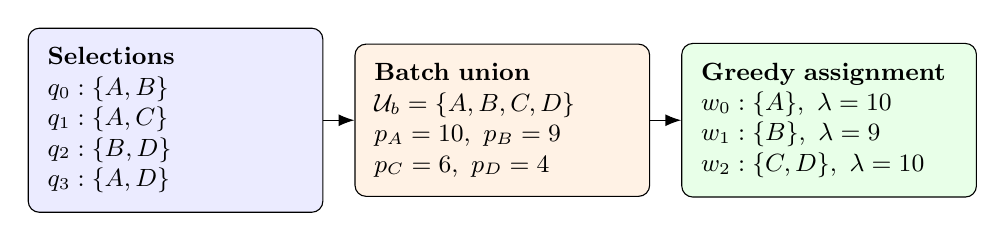
\begin{tikzpicture}[font=\small,>=Latex]
\node[draw,rounded corners,fill=blue!8,align=left,text width=3.25cm,
      inner sep=7pt] (selected) at (-4.15,0) {
\textbf{Selections}\par
\(q_0:\{A,B\}\)\par
\(q_1:\{A,C\}\)\par
\(q_2:\{B,D\}\)\par
\(q_3:\{A,D\}\)};

\node[draw,rounded corners,fill=orange!10,align=left,text width=3.25cm,
      inner sep=7pt] (union) at (0,0) {
\textbf{Batch union}\par
\(\mathcal U_b=\{A,B,C,D\}\)\par
\(p_A=10,\ p_B=9\)\par
\(p_C=6,\ p_D=4\)};

\node[draw,rounded corners,fill=green!9,align=left,text width=3.25cm,
      inner sep=7pt] (workers) at (4.15,0) {
\textbf{Greedy assignment}\par
\(w_0:\{A\},\ \lambda=10\)\par
\(w_1:\{B\},\ \lambda=9\)\par
\(w_2:\{C,D\},\ \lambda=10\)};

\draw[-{Latex[length=2mm]}] (selected.east) -- (union.west);
\draw[-{Latex[length=2mm]}] (union.east) -- (workers.west);
\end{tikzpicture}
\caption{Pedagogical four-query example of batch-level list union and greedy
whole-list scheduling. The real implementation uses batches of up to 32
queries and all configured fine-search workers. Each selected list is an
indivisible task weighted by its padded number of candidate pages.}
\label{fig:pedagogical-list-scheduling}
\end{figure}

The page count is an estimate rather than a cycle-accurate cost model. It does not capture per-list setup, masking of the final partial page, variation in memory service time, circular-buffer waiting, or synchronization. Moreover, because a large inverted list cannot be divided, the longest list can still determine the batch completion time. After scheduling, the host serialises one description per fine-search worker so that its reader kernel can locate the assigned complete lists in device memory.

\subsection{Worker Description}
\label{subsec:worker-description}

The host serialises the fine-search assignment into one logical flattened worker description in DRAM for each fine-search worker. A description can span multiple DRAM pages, so it is not restricted to one physical page. It contains the information required by the reader kernel to locate the query batches and the complete inverted lists assigned to that worker.

Let \(B\) denote the number of query batches, as introduced in Section~\ref{subsec:end-to-end-pipeline}. The worker description has the conceptual form
\begin{equation}
W_w
=
\left\langle
B,\,
R_0,\,
R_1,\,
\ldots,\,
R_{B-1}
\right\rangle,
\label{eq:worker-description}
\end{equation}
where \(R_b\) describes the work assigned to worker \(w\) for query batch \(b\).

Each batch record contains the global offset of the query batch in the query buffer, the number of tiles used to represent it, and the number of whole-list tasks that the worker must process:
\begin{equation}
R_b
=
\left\langle
o^{Q}_b,\,
n^{Q}_b,\,
N^{(w)}_{\mathrm{list},b},\,
E^{(w)}_{b,0},\,
E^{(w)}_{b,1},\,
\ldots,\,
E^{(w)}_{b,N^{(w)}_{\mathrm{list},b}-1}
\right\rangle,
\label{eq:worker-batch-record}
\end{equation}
where \(o^{Q}_b\) is the global offset of query batch \(b\) in the query buffer, \(n^{Q}_b\) is the number of tiles composing its padded representation, and \(N^{(w)}_{\mathrm{list},b}\) is the number of whole-list tasks assigned to worker \(w\) for that batch.

Each whole-list entry \(r\) is represented as
\begin{equation}
E^{(w)}_{b,r}
=
\left\langle
o^{V}_{b,r},\,
n^{V}_{b,r}
\right\rangle,
\label{eq:worker-list-record}
\end{equation}
where \(o^{V}_{b,r}\) is the global candidate-page offset of the assigned inverted list in the packed database buffer, and \(n^{V}_{b,r}\) is the number of candidate pages in that complete list. Although the record is encoded as an offset and page-count pair, it always describes an entire selected list; the scheduler does not create subranges. Since each candidate page contains 32 vectors, these two values are sufficient for the reader kernel to determine where the list begins and how many candidate-vector and identifier tiles must be fetched from their respective packed buffers.

At the beginning of fine search, each worker copies its description from DRAM into local L1. For each batch with assigned work, the corresponding query tiles are loaded once into the local query circular buffer and remain resident while all whole-list tasks associated with that batch are processed. The reader then advances to the next batch record and repeats the same procedure.

\section{Fine Search and Result Reduction}
\label{sec:fine-search-and-reduction}

\subsection{Worker Pipeline}
\label{subsec:fine-worker-pipeline}

The fine-search program evaluates the candidate pages selected by the host schedule. As defined above, logical core \((0,0)\) performs final aggregation, while the other 63 cores in the configured \(8\times8\) logical grid operate as fine-search workers.

Each worker executes reader, compute, and writer kernels concurrently. At the beginning of the invocation, the reader loads the worker description from DRAM into local L1; for each active query batch, the query tiles are then loaded once into the worker's query circular buffer and retained while all candidate pages assigned to that worker for the batch are processed.

Candidate vectors and their identifier tiles are streamed from the packed DRAM buffers. The reader issues both reads before a shared synchronization barrier, allowing their transfers over the on-device Network-on-Chip (NoC) to be outstanding concurrently. Double-buffering of the candidate circular buffers allows the reader to prepare a later page while the compute kernel operates on an earlier one, subject to circular-buffer capacity and producer--consumer synchronization.

Let \(j\) identify a whole inverted-list task assigned to the worker and let \(p\) identify a candidate page within that list. For one such page \(V_{j,p}\in\mathbb{R}^{D_{\mathrm{p}}\times32}\), the compute kernel evaluates
\begin{equation}
S^{\mathrm{fine}}_{b,j,p}=Q_bV_{j,p},
\label{eq:fine-search}
\end{equation}
producing a \(32\times32\) tile of query--candidate similarities.

Across all candidate pages assigned to it, the worker incrementally maintains a row-wise top-32 state, with scores and original vector identifiers propagated together through the same ordering operations. No list-local to global identifier reconstruction is therefore required after the search.

Figure~\ref{fig:fine-local-topk} shows the local top-32 update performed by one fine-search worker. Two \(32\times32\) tiles hold the best scores and identifiers found so far, while the other two contain the scores and identifiers of the current candidate page. Before selection, the current and saved score and identifier tiles are transposed so that each column corresponds to one query and the rows contain candidate entries. The compute-kernel \texttt{topk\_local\_sort} operation then applies the same ordering decisions to the score and identifier tiles, preserving the association between every similarity value and its original vector identifier.

\begin{figure}[htbp]
\centering
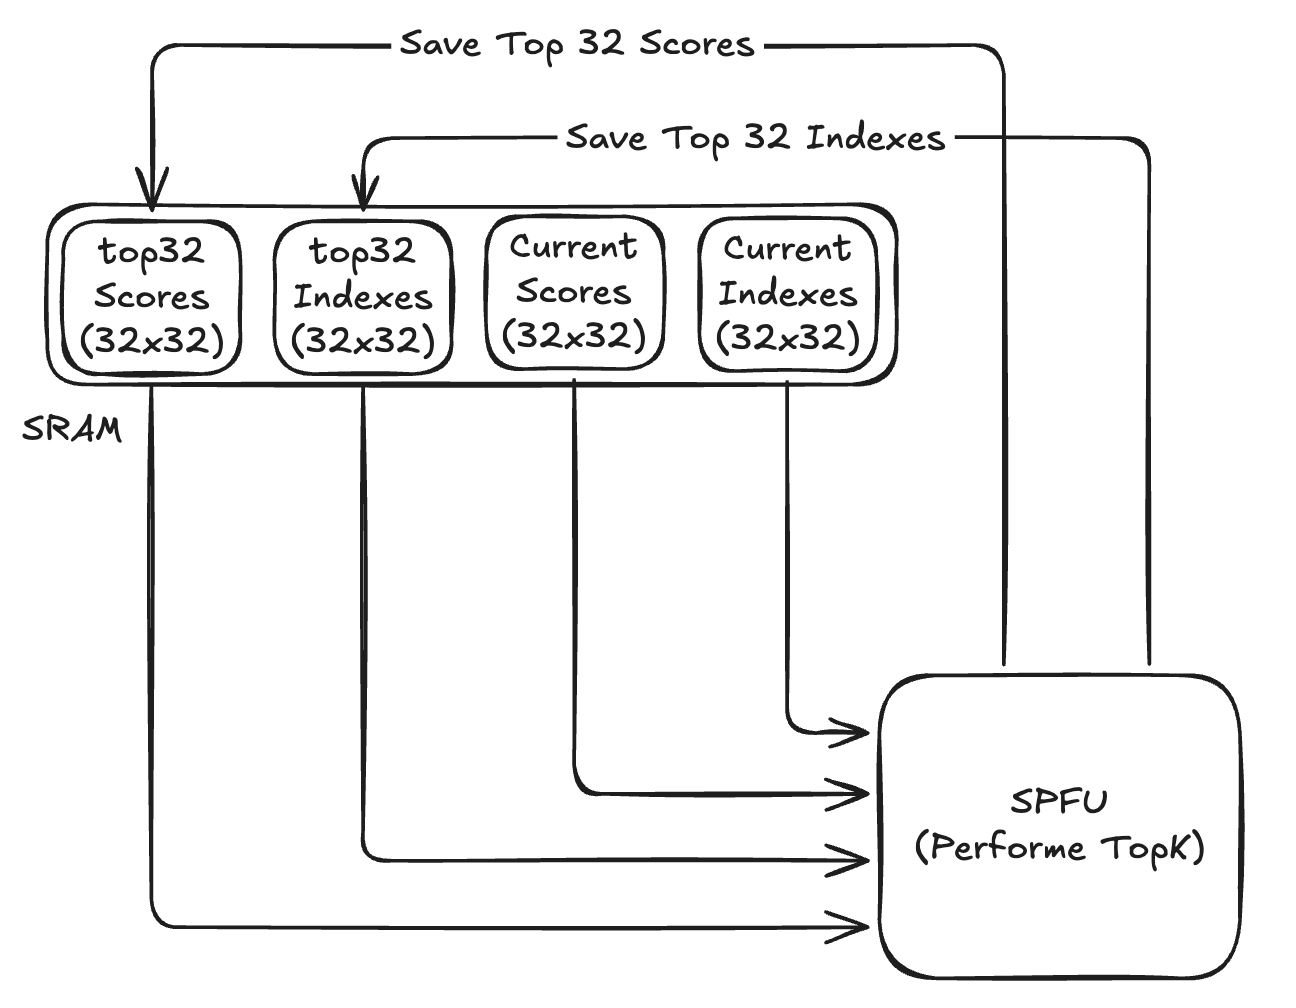
\includegraphics[width=0.78\textwidth]{./assets/fine_search_local_topk.png}
\caption{Worker-local top-32 update. Before selection, the score and identifier tiles are transposed so that each column corresponds to one query and the rows contain candidate entries from the saved and current states. The \texttt{topk\_local\_sort} operation applies identical ordering decisions to scores and identifiers.}
\label{fig:fine-local-topk}
\end{figure}

\subsection{Hierarchical Top-\texorpdfstring{\(k\)}{k}}
\label{subsec:hierarchical-topk}

A single worker observes only part of the candidate set, so the final result is computed hierarchically. For query row \(r\) in batch \(b\), worker \(w\) first retains
\begin{equation}
R_{b,w,r}=\operatorname{Top}_{32}\left(\mathcal{C}_{b,w,r}\right),
\label{eq:worker-top32}
\end{equation}
where \(\mathcal{C}_{b,w,r}\) is the set of candidates evaluated by that worker.

Worker-local results are staged in DRAM, with each configured worker writing one fixed-size score tile and one identifier tile per query batch to a region indexed by batch and worker. All configured workers produce and signal one partial result for every batch, even when a worker has no active list task for that batch. In that case, every score remains at the initial value \(-10000\) and every identifier remains at \texttt{0xffffffff}.

Synchronization uses a cumulative completion semaphore in the L1 memory of logical core \((0,0)\). After writing its partial result for a batch, each worker increments this semaphore, and the aggregation reader waits until the expected number of increments has been observed. Once the partial result of a worker has been consumed, the aggregation reader increments a worker-specific ready semaphore in that worker's L1 memory, allowing the worker to reuse its partial-result slot and advance to the next batch.

Figure~\ref{fig:fine-partial-staging} illustrates this two-way handshake. Fine-search workers write their local top-32 results to distinct locations in the shared DRAM partial-result buffer and signal completion to the aggregation core; after consuming those results, core \((0,0)\) signals the corresponding workers that their slots can be reused.

\begin{figure}[htbp]
\centering
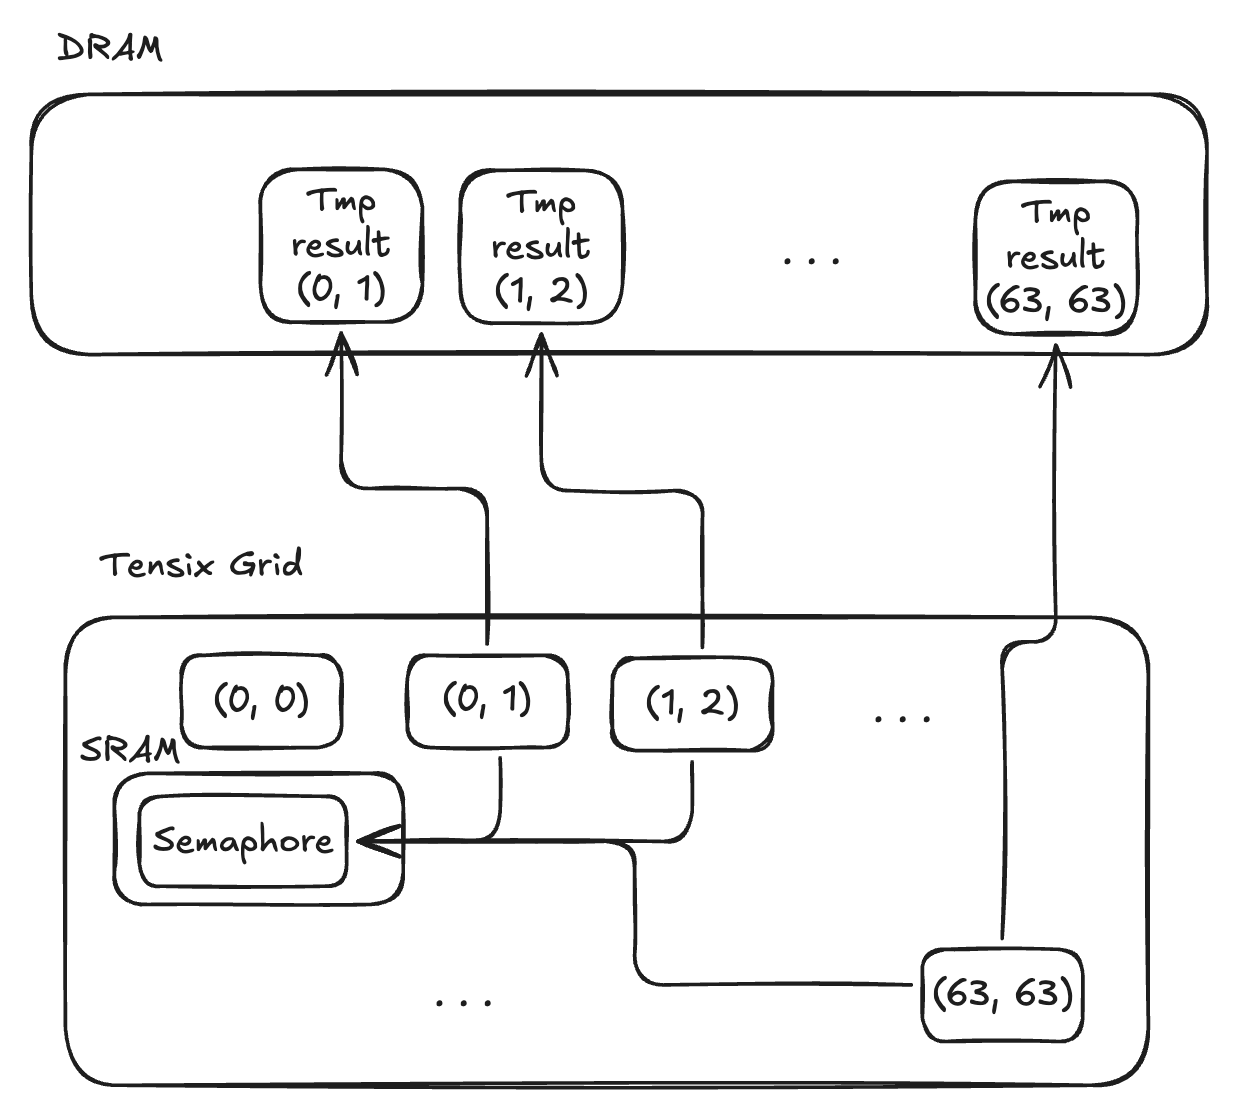
\includegraphics[width=0.78\textwidth]{./assets/fine_search_partial_results.png}
\caption{DRAM staging and synchronization of fine-search partial results. Workers store their local top-32 results in DRAM and synchronize with the aggregation core through completion and ready semaphores.}
\label{fig:fine-partial-staging}
\end{figure}

The aggregation compute kernel performs the second reduction,
\begin{equation}
R_{b,r}=\operatorname{Top}_{32}\left(\bigcup_w R_{b,w,r}\right),
\label{eq:global-top32}
\end{equation} and writes one final score tile and one final identifier tile per batch to DRAM. Figure~\ref{fig:pedagogical-hierarchical-topk} reduces the tile width from 32 to 4 to illustrate the two-level selection without the visual complexity of the actual result tiles.

\begin{figure}[htbp]
\centering
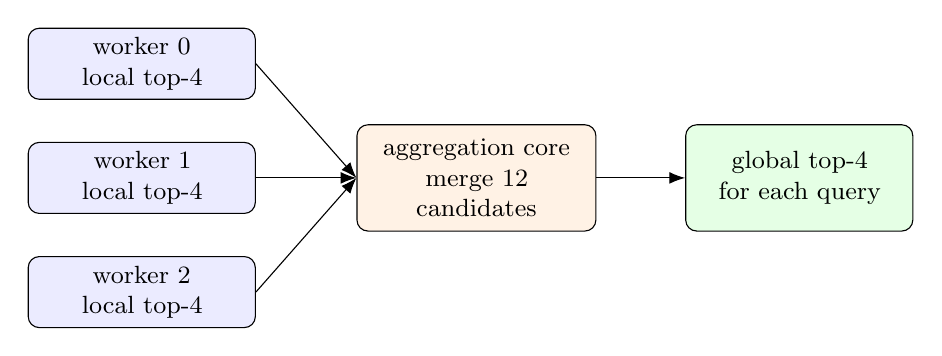
\begin{tikzpicture}[font=\small,>=Latex]
\node[draw,rounded corners,fill=blue!8,align=center,text width=2.65cm]
  (w0) at (-4.25,1.45) {worker 0\\local top-4};
\node[draw,rounded corners,fill=blue!8,align=center,text width=2.65cm]
  (w1) at (-4.25,0) {worker 1\\local top-4};
\node[draw,rounded corners,fill=blue!8,align=center,text width=2.65cm]
  (w2) at (-4.25,-1.45) {worker 2\\local top-4};

\node[draw,rounded corners,fill=orange!10,align=center,text width=2.8cm,
      minimum height=1.35cm] (merge) at (0,0)
  {aggregation core\\merge 12 candidates};
\node[draw,rounded corners,fill=green!10,align=center,text width=2.65cm,
      minimum height=1.35cm] (final) at (4.1,0)
  {global top-4\\for each query};

\draw[-{Latex[length=2mm]}] (w0.east) -- (merge.west);
\draw[-{Latex[length=2mm]}] (w1.east) -- (merge.west);
\draw[-{Latex[length=2mm]}] (w2.east) -- (merge.west);
\draw[-{Latex[length=2mm]}] (merge.east) -- (final.west);
\end{tikzpicture}
\caption{Pedagogical two-level result reduction for three workers, retaining
four entries. Each worker first retains its local best four candidates;
logical core \texttt{(0,0)} merges the partial results and retains the global
best four for each query. The implementation uses top-32 states and all
configured workers.}
\label{fig:pedagogical-hierarchical-topk}
\end{figure}

The host converts the tiled outputs to row-major form, removes sentinel entries, discards padded query rows, and retains the first \(k\) results for every valid query. The implementation therefore supports \(k\leq32\); the evaluation in this thesis uses \(k=10\).

For \(B\) query batches and \(W\) fine-search workers, logical core \((0,0)\) consumes \(BW\) worker-result pairs and performs \(BW\) running top-32 updates. Synchronization activity and partial-result traffic also grow linearly with the number of worker results. With \(W=63\), each batch contributes 63 score-and-identifier result pairs to the aggregation stage and requires 63 running top-32 updates. Because workers without active list tasks still write sentinel results, this cost depends on the configured worker count rather than the number of non-empty assignments. The centralised stage consequently scales as \(\Theta(BW)\) and can constrain designs with larger worker counts.

\section{Multi-Batch Execution}
\label{sec:multi-batch-execution}

The first implementation processed one batch of at most 32 queries per search invocation. This design matched the \(32\times32\) tile representation and simplified the initial implementation, but a larger query workload required the host to repeat query preparation, coarse execution, synchronization, list selection, fine-search scheduling, fine execution, final result transfer, and host-side orchestration for every group of 32 queries.

The final implementation, represented by \texttt{ann\_ivf\_dram\_args}, retains the same 32-query internal representation while allowing one search call to process multiple batches. After a coarse-search invocation processes all valid batches of the workload, the host constructs the fine-search descriptions for the complete set of selected lists. These logical descriptions may occupy multiple DRAM pages, so the format does not impose a fixed batch-count limit. The fine-search program then processes the paged descriptions within one larger invocation; practical capacity remains bounded by the device-memory allocation available to the workload.

This change separates tile size from execution granularity: a batch of 32 queries remains the natural unit of matrix computation, but it is no longer the unit at which the complete device pipeline must be launched. Repeated program configuration, launch, synchronization, and host orchestration are consequently amortised across a larger number of queries.

\section{Implementation Constraints}
\label{sec:implementation-constraints}

Table~\ref{tab:implementation-constraints} consolidates the implementation constraints derived in the preceding sections without repeating their full derivations.

\begin{table}[htbp]
\centering
\caption{Principal constraints of the evaluated Tenstorrent implementation.}
\label{tab:implementation-constraints}
\small
\setlength{\tabcolsep}{5pt}
\renewcommand{\arraystretch}{1.12}
\begin{tabularx}{\textwidth}{p{0.22\textwidth} p{0.31\textwidth} X}
\toprule
Constraint & Cause & Consequence \\
\midrule
Tile alignment
& The compute path operates on \(32\times32\) tiles.
& Vector dimensions and list lengths are padded to multiples of 32; an
  internal query batch contains up to 32 valid queries. \\

Centroid blocking
& Coarse search traverses complete 32-centroid blocks.
& The current representation requires \(N_{\mathrm{list}}\) to be divisible
  by 32. \\

Selection capacity
& Coarse, worker-local, and global selection use top-32 states.
& \(N_{\mathrm{probe}}\leq32\) and \(k\leq32\). The reported experiments use
  \(k=10\). \\

Whole-list scheduling
& A worker record addresses one complete inverted list.
& Lists cannot be split across workers, so a large list can determine the
  batch tail even after greedy balancing. \\

Paged worker descriptions
& A logical description may span multiple DRAM pages.
& The format imposes no fixed batch-count limit; practical capacity depends
  on the device-memory allocation available to the invocation. \\

Centralised reduction
& Every worker emits one partial result for every batch.
& Aggregation work and intermediate traffic scale as \(\Theta(BW)\), including
  sentinel results from workers with empty assignments. \\

Deployment scope
& The implementation targets one Wormhole n150 device.
& Multi-device approximate nearest-neighbour execution is outside the scope
  of this work. \\
\bottomrule
\end{tabularx}
\end{table}

Reader, compute, and writer kernels additionally share the local L1 capacity through their circular buffers, query tiles, intermediate similarities, identifier tiles, running top-32 states, and worker metadata. Buffer depth must therefore balance query reuse and double buffering against local-memory capacity. Progress also remains subject to circular-buffer backpressure, NoC completion, and the synchronization dependencies described above.

\section{Chapter Summary}
\label{sec:design-summary}

This chapter described the implementation of IVF-Flat search on a single-chip Tenstorrent Wormhole n150 device, with the index transformed into a tile-oriented representation in which vectors are grouped by inverted list and stored in 32-vector pages together with their original identifiers.

The search pipeline is divided into a regular coarse-search phase and an irregular fine-search phase. While coarse search reuses query tiles to scan the centroid matrix and return a fixed-size set of centroid candidates, the host subsequently selects the \(N_{\mathrm{probe}}\) lists, forms batch-level unions, and assigns complete selected lists to workers using their padded page counts as weights in a greedy longest-task-first scheduler.

Each fine-search worker reuses one query batch while streaming the candidate pages of its assigned lists and maintaining a worker-local row-wise top-32 state. The resulting partial results are staged in DRAM and merged on logical core \((0,0)\) before the final outputs are returned to the host.

The final design preserves the natural 32-query tile representation while extending execution to multiple batches per invocation. This reduces repeated host--device orchestration while preserving the same coarse- and fine-search stages and using batch-level list unions to match the tile-oriented execution model. The following chapter defines the methodology used to evaluate the resulting implementation.


%\hypersetup{colorlinks=true, linkcolor=blue, citecolor=red}

\chapter{Experiments Methodology}
\section{Evaluation Goals}

\section{Hardware and Software Configuration}
Specify HW components used and clusters

\section{Dataset and Index Parameters}
Explicit parameters passed and explain well also based on the job file

\section{Recall and Performance Metrics}

\section{Benchmark Procedure}

\section{Power and Energy Measurement}
Same as before say as good as possible as before it based on the job file also saying the different workload.
Usa anche il tool
Also show that we used CPU + GPU time for the GPU b/c ...
Say the difference between CPU and TT/GPU for power measurement, aka Jouls vs Energy run base on integral of Power Samples.


\cleardoublepage

%\chapter{Experimental Results}
\label{chap:results}

This chapter compares throughput at measured recall, analyzes the effect of
\(N_{\mathrm{list}}\) and \(N_{\mathrm{probe}}\), decomposes the Tenstorrent
search path, and reports workload energy. Throughput is the median of ten
search-only repetitions, whereas energy covers the complete 100,000-query
session of Equation~\ref{eq:queries-per-run}, including initialization.

\section{CPU, GPU, and Tenstorrent Comparison}
\label{sec:cross-platform-performance}

Figure~\ref{fig:qps-recall} shows QPS against measured Recall@10 on a
logarithmic throughput axis. Placing recall rather than
\(N_{\mathrm{probe}}\) on the horizontal axis allows the Tenstorrent
batch-union implementation to be compared with per-query IVF search without
assuming equivalent candidate sets. Table~\ref{tab:qps-matched} extracts the
four recall-matched operating points of Table~\ref{tab:recall-matched-points}.

\begin{figure}[htbp]
\centering
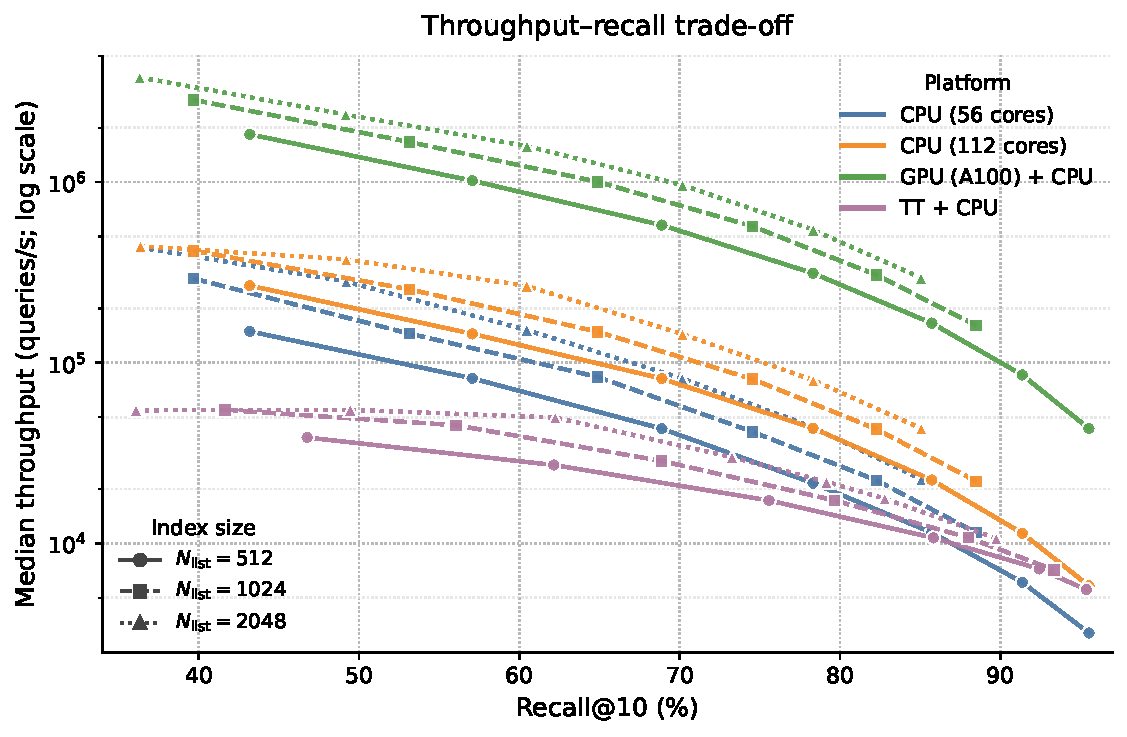
\includegraphics[width=0.94\textwidth]{./assets/qps_vs_recall.pdf}
\caption{Queries per second versus measured Recall@10. Each point is the median
of ten repetitions, and lines connect \(N_{\mathrm{probe}}\) values within one
\(N_{\mathrm{list}}\) sweep. The Tenstorrent \((2048,12)\) energy-matching point
is included; other exploratory \(N_{\mathrm{probe}}=12\) runs are not.}
\label{fig:qps-recall}
\end{figure}

\begin{table}[htbp]
\centering
\caption{Median search throughput at the recall-matched operating points of
Table~\ref{tab:recall-matched-points}. The ratio is baseline QPS divided by
Tenstorrent QPS, so values above one favor the baseline.}
\label{tab:qps-matched}
\small
\setlength{\tabcolsep}{4pt}
\renewcommand{\arraystretch}{1.08}
\begin{tabular}{lrrrrrrr}
\toprule
& \multicolumn{4}{c}{Median QPS} & \multicolumn{3}{c}{Ratio to TT} \\
\cmidrule(lr){2-5}\cmidrule(lr){6-8}
Target & CPU (56) & CPU (112) & A100 & TT & CPU (56) & CPU (112) & A100 \\
\midrule
60\% & 151,858 & 266,184 & 1,583,712 & 49,720 & 3.05 & 5.35 & 31.85 \\
78\% & 43,864  & 80,075  & 544,703   & 21,907 & 2.00 & 3.66 & 24.86 \\
88\% & 11,466  & 22,079  & 160,799   & 10,762 & 1.07 & 2.05 & 14.94 \\
95\% & 3,190   & 5,822   & 43,271    & 5,550  & 0.57 & 1.05 & 7.80 \\
\bottomrule
\end{tabular}
\end{table}

The GPU is the fastest configuration across the whole recall range, by a
factor of 31.9 over Tenstorrent at the 60\% target and 7.8 at the 95\% target.
Tenstorrent is also slower than both CPU configurations up to about 88\%
recall: the 56-core CPU is 3.05 times faster at 60\% and reaches parity at
88\%, while the 112-core CPU remains 2.05 times faster at 88\%. The crossover
with the 56-core CPU lies near 90\% recall: Tenstorrent at \((512,16)\) reaches
92.4\% recall at 7,229~QPS, whereas the CPU reaches 91.4\% at 6,090~QPS with
\((512,32)\). At the 95\% target, Tenstorrent is 1.74 times faster than the
56-core CPU and within 5\% of the 112-core CPU. These comparisons hold against
the evaluated grid: near 95\% recall the only Faiss point is \((512,64)\),
whereas Section~\ref{sec:nlist-nprobe-results} shows that Faiss is faster with
more lists, so configurations with more lists and larger
\(N_{\mathrm{probe}}\), which were not evaluated, could narrow or reverse the
CPU comparison. Within the evaluated grid, Tenstorrent's relative position
improves steadily with recall, because its throughput falls more
slowly than that of the baselines as search depth grows. When
\(N_{\mathrm{probe}}\) doubles, Faiss scans twice as many lists for every
query, and its throughput roughly halves: at 512 lists, going from
\(N_{\mathrm{probe}}=16\) to 32 lowers it by a factor of 1.89 on the 56-core
CPU. On Tenstorrent, the work per batch is set by the union of the lists
selected by its queries, and the additional lists increasingly overlap with
those already selected by other queries, so the union grows by much less than
a factor of two (Section~\ref{sec:nlist-nprobe-results}). At 512 lists, its
pages grow by a factor of 1.51 from \(N_{\mathrm{probe}}=8\) to 16 and of 1.31
from 16 to 32, and the throughput falls by almost the same factors, 1.49 and
1.30. At low recall, however, Tenstorrent is limited by a fixed per-batch cost,
also analyzed in Section~\ref{sec:nlist-nprobe-results}.

The 112-core CPU is faster than the 56-core CPU at every configuration, but
the speed-up depends on the amount of work per query. It is small when little
candidate work is available, only 1.02 at \((2048,1)\), 1.33 at
\((2048,2)\), and 1.42 at \((1024,1)\), because per-call overheads then
dominate. With more work it
lies between 1.75 and 2.01 without a monotonic trend, peaking at \((512,8)\).
Near-linear and occasionally slightly super-linear scaling is consistent with
the larger aggregate cache and memory bandwidth available to the full node.

Run-to-run variation is small compared with the differences between
platforms. Across the complete grid, the QPS RSD of
Equation~\ref{eq:qps-rsd} is at most 4.64\% for the 56-core CPU, 5.89\% for
the 112-core CPU, 2.43\% for the GPU, and 1.46\% for Tenstorrent, and the
ten repetitions show no systematic first-repetition slowdown. The medians in
Figure~\ref{fig:qps-recall} and Table~\ref{tab:qps-matched} are therefore
not driven by individual repetitions.

\section{Impact of \texorpdfstring{\(N_{\mathrm{list}}\) and
\(N_{\mathrm{probe}}\)}{Nlist and Nprobe}}
\label{sec:nlist-nprobe-results}

Within every sweep, increasing \(N_{\mathrm{probe}}\) raises recall and lowers
throughput. The choice of \(N_{\mathrm{list}}\), however, affects the platforms
differently.

\paragraph{Faiss favors finer partitions.}
At matched recall, the Faiss baselines are faster with more lists. Near 78\%
recall, the GPU reaches 544,703~QPS at \((2048,16)\) but only 313,161~QPS at
\((512,8)\), a factor of 1.74; the gain is 2.03 on the 56-core CPU and 1.84 on the
112-core CPU.
Smaller lists reduce the candidate volume per probe more than the larger
coarse scan costs.

\paragraph{The batch union raises Tenstorrent recall.}
Table~\ref{tab:union-recall-gain} compares Tenstorrent and Faiss recall at the
same configuration. Because every query is also scored against lists selected
by other queries in its batch, Tenstorrent is more accurate at almost every
point, by up to 7.52 percentage points at \((512,8)\). The gain first grows
with \(N_{\mathrm{probe}}\) and then shrinks as recall approaches saturation.
It also decreases with \(N_{\mathrm{list}}\): the maximum is 7.52 points for
512 lists, 5.74 for 1024, and 4.67 for 2048. This is consistent with lists
contributed by other queries being less likely to contain a query's true
neighbors when the partition is finer.

\begin{table}[htbp]
\centering
\caption{Recall@10 difference, Tenstorrent minus Faiss CPU, in percentage
points at equal \((N_{\mathrm{list}},N_{\mathrm{probe}})\).}
\label{tab:union-recall-gain}
\small
\setlength{\tabcolsep}{6pt}
\renewcommand{\arraystretch}{1.08}
\begin{tabular}{lrrrrrr}
\toprule
& \multicolumn{6}{c}{\(N_{\mathrm{probe}}\)} \\
\cmidrule(lr){2-7}
\(N_{\mathrm{list}}\) & 1 & 2 & 4 & 8 & 16 & 32 \\
\midrule
512  & \(+3.58\) & \(+5.08\) & \(+6.68\) & \(+7.52\) & \(+6.71\) & \(+4.00\) \\
1024 & \(+1.95\) & \(+2.89\) & \(+4.00\) & \(+5.12\) & \(+5.74\) & \(+4.85\) \\
2048 & \(-0.27\) & \(+0.25\) & \(+1.78\) & \(+3.10\) & \(+4.46\) & \(+4.67\) \\
\bottomrule
\end{tabular}
\end{table}

\paragraph{The union multiplies the scanned data.}
The recall gain has a cost. Figure~\ref{fig:union-scanned-fraction} and
Table~\ref{tab:union-scan} compare the fraction of the database against which
each query is scored on Tenstorrent, whose queries scan the whole batch union,
with the fraction that Faiss scans through the query's own
\(N_{\mathrm{probe}}\) lists. Both use the lists selected by the Tenstorrent
coarse search, logged on the host for one repetition of 10,000 queries; the
batching is deterministic, and a repeated run produced identical unions. At
equal parameters, a Tenstorrent query is scored against 12 to 32 times as many
vectors as a Faiss query. At the four energy operating points it scans 6.7\%,
18.3\%, 41.0\%, and 81.7\% of the database, so at the 95\% target the fine
search is close to an exhaustive scan.

\begin{figure}[htbp]
\centering
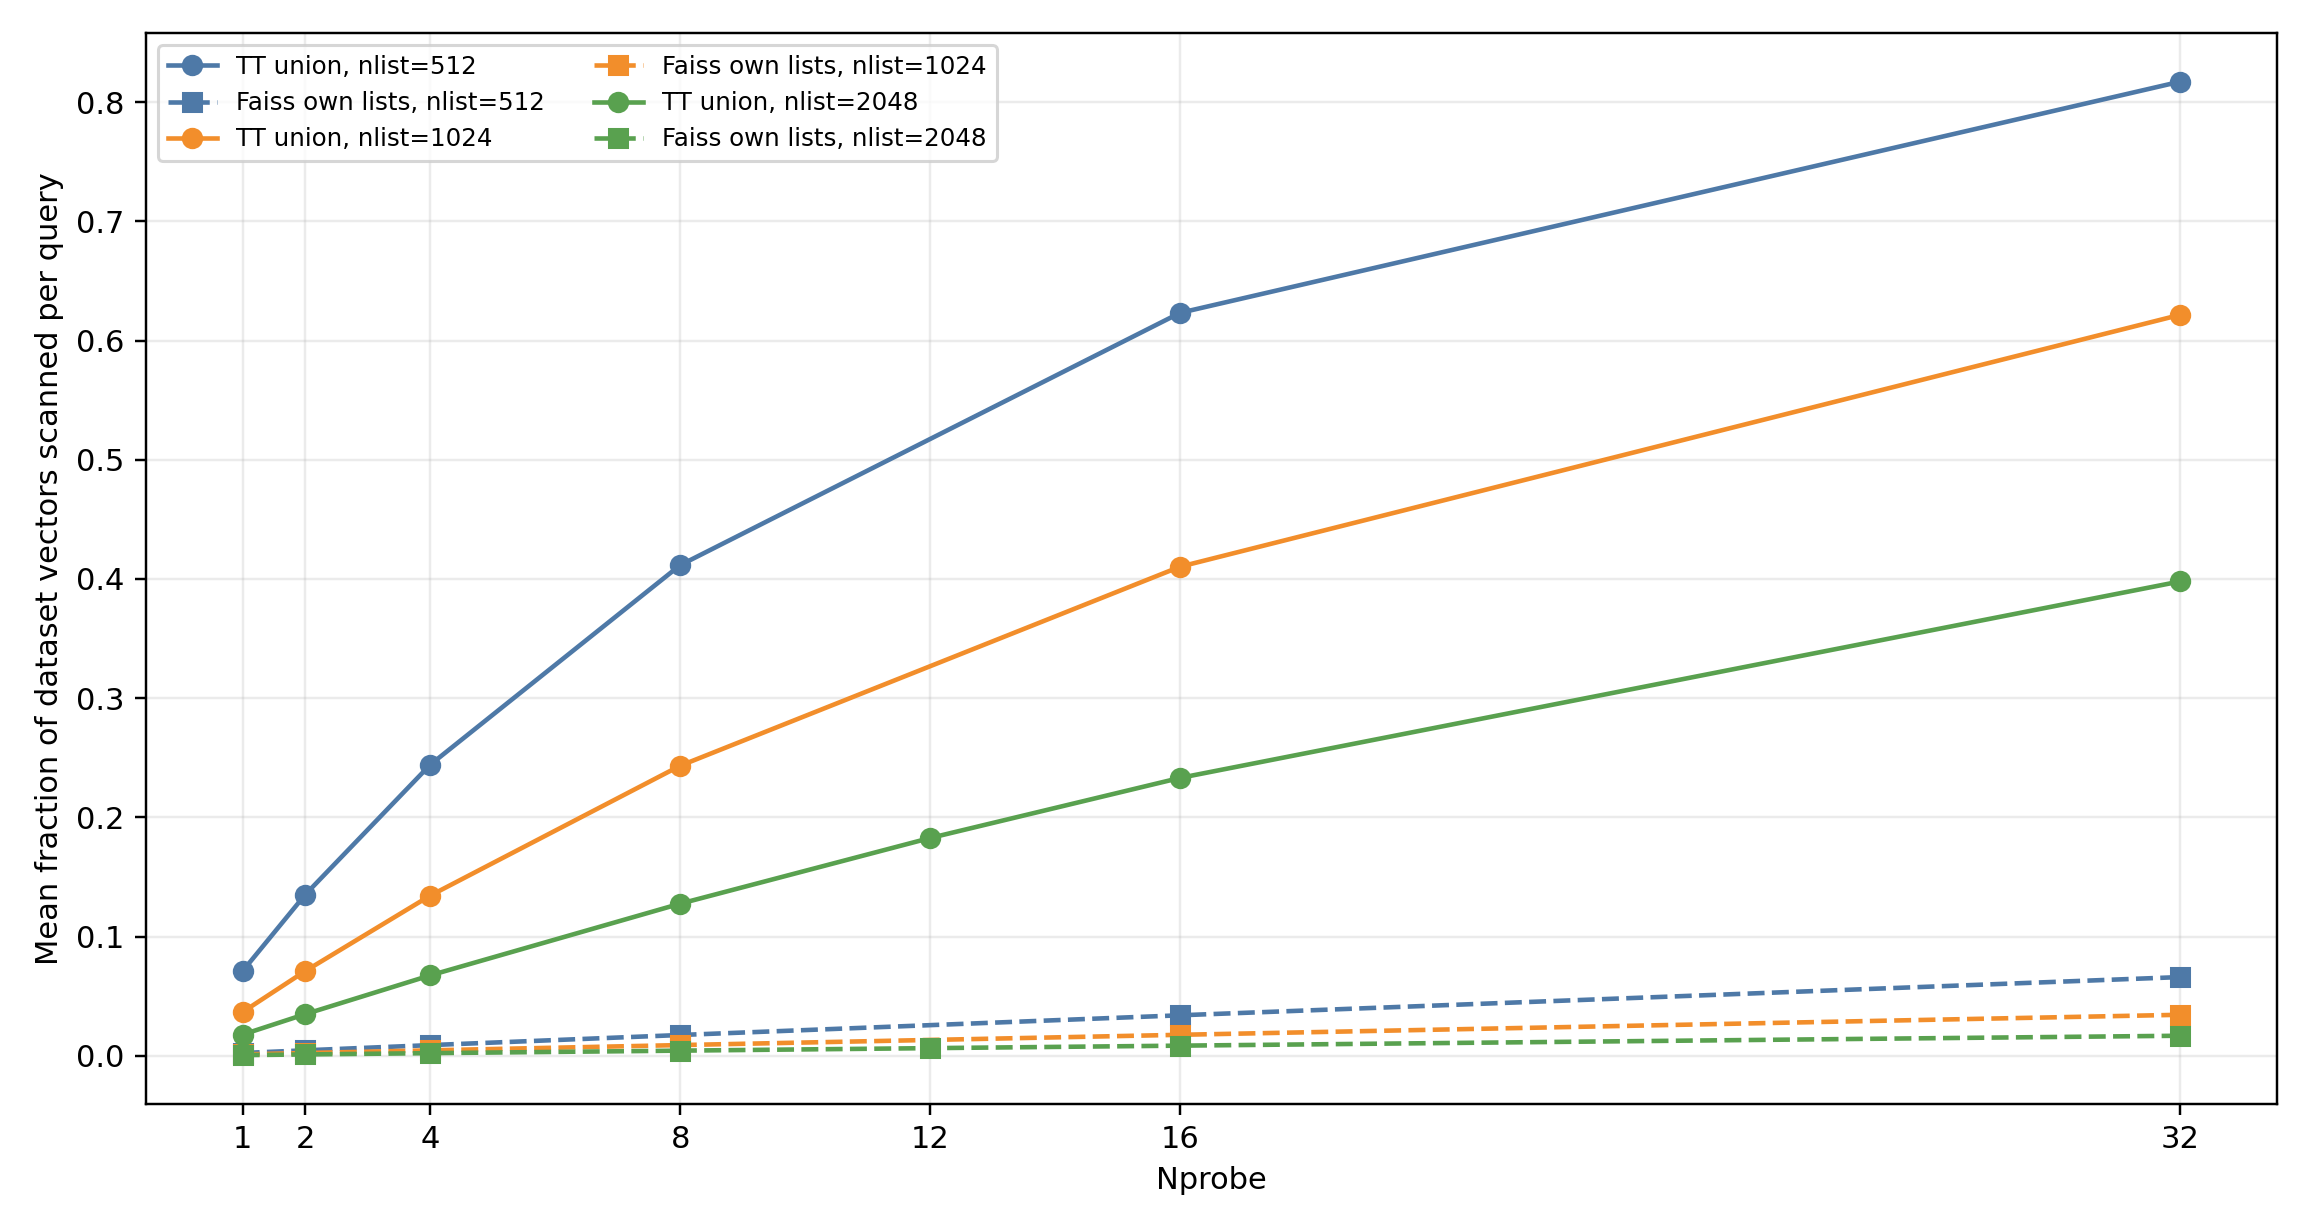
\includegraphics[width=0.94\textwidth]{./assets/union_scanned_fraction.png}
\caption{Mean fraction of the database scanned per query as a function of
\(N_{\mathrm{probe}}\): the batch union on Tenstorrent (solid) and the query's
own lists as in Faiss (dashed), for each \(N_{\mathrm{list}}\).}
\label{fig:union-scanned-fraction}
\end{figure}

\begin{table}[htbp]
\centering
\caption{Mean fraction of the database scanned per query on Tenstorrent, and
the factor by which it exceeds the vectors in the query's own
\(N_{\mathrm{probe}}\) lists. A factor of 32 means that the 32 queries of a
batch share no lists.}
\label{tab:union-scan}
\small
\setlength{\tabcolsep}{5pt}
\renewcommand{\arraystretch}{1.08}
\begin{tabular}{llrrrrrrr}
\toprule
& & \multicolumn{7}{c}{\(N_{\mathrm{probe}}\)} \\
\cmidrule(lr){3-9}
\(N_{\mathrm{list}}\) & & 1 & 2 & 4 & 8 & 12 & 16 & 32 \\
\midrule
512  & scanned & 7.1\% & 13.5\% & 24.4\% & 41.1\% & -- & 62.3\% & 81.7\% \\
     & factor  & 30.6 & 29.5 & 27.3 & 23.6 & -- & 18.3 & 12.4 \\
\midrule
1024 & scanned & 3.7\% & 7.1\% & 13.4\% & 24.3\% & -- & 41.0\% & 62.1\% \\
     & factor  & 31.2 & 30.6 & 29.4 & 27.1 & -- & 23.3 & 18.1 \\
\midrule
2048 & scanned & 1.8\% & 3.5\% & 6.7\% & 12.8\% & 18.3\% & 23.3\% & 39.8\% \\
     & factor  & 31.6 & 31.3 & 30.7 & 29.6 & 28.5 & 27.4 & 23.7 \\
\bottomrule
\end{tabular}
\end{table}

The factors close to 32 show that consecutive queries in dataset order share
almost no lists. At \((2048,4)\), for example, the 128 lists requested by a
batch contain a median of 124 distinct lists. Overlap appears only when the
union covers a large part of all lists, as at \((512,32)\), where 1,024
selections contain a median of 412 distinct lists, or 80\% of the 512. This
explains the recall gain of Table~\ref{tab:union-recall-gain}, which is bought
with a much larger scan, and why the gain falls with finer partitions, where
each extra list covers a smaller part of the database. It also explains why
Tenstorrent's position against the CPUs improves with recall: its scanned
volume approaches the whole database and grows slowly, whereas the per-query
scan of Faiss keeps growing with \(N_{\mathrm{probe}}\).

The union is nevertheless the right choice for the device. Every query must
still be scored against its own \(N_{\mathrm{probe}}\) lists, and each
fine-search step multiplies a full 32-query tile regardless of how many rows
are useful. Processing the queries separately would therefore fetch and
multiply every selected list once per query that requests it, whereas the
union fetches each distinct list only once per batch. The number of pages
fetched falls by the overlap factor, the ratio of requested to distinct lists,
and the extra candidates that each query receives come from lists fetched for
other queries at no additional matrix multiplication. In dataset order,
however, the overlap factor is only 1.0--2.5, so the saving is small; grouping
queries that select similar lists into the same batch would raise it.

\paragraph{Tenstorrent sweeps converge at high recall.}
Above about 85\% recall, the three Tenstorrent sweeps nearly coincide:
\((512,8)\), \((1024,16)\), and \((2048,32)\) all run at about 10,700~QPS and
reach 85.83\%, 88.03\%, and 89.75\% recall respectively. In this regime
\(N_{\mathrm{list}}\) mainly shifts recall at similar cost, and 2048 lists give
the best trade-off.

\paragraph{Tenstorrent has a fixed per-batch floor.}
At low \(N_{\mathrm{probe}}\), Tenstorrent throughput stops increasing:
\((1024,1)\), \((2048,1)\), and \((2048,2)\) all run at about 54,800~QPS, or
about 182~ms per 10,000 queries, even though their candidate volumes differ.
This corresponds to roughly 0.58~ms per 32-query batch that does not depend on
\(N_{\mathrm{probe}}\). At 2048 lists the most likely cause is the final
aggregation. The
aggregation core processes the batches one after another, and for every batch
it merges one top-32 result from each of the 63 workers, including workers
without assigned lists (Section~\ref{subsec:hierarchical-topk}). In the batch
trace of Section~\ref{subsec:tt-device-timeline-results} this takes about
0.44~ms per batch, close to the floor. At larger \(N_{\mathrm{probe}}\) the
workers need several milliseconds per batch, so the aggregation overlaps with
their work and is not a bottleneck; at low \(N_{\mathrm{probe}}\) the workers
finish a batch sooner than the aggregation, which then becomes a likely
bottleneck. This floor caps Tenstorrent's low-recall throughput and explains
much of its gap to the CPUs at the 60\% target. Load imbalance contributes as
well: at \(N_{\mathrm{probe}}=1\) a batch union holds at most 32 lists, so at
most 32 of the 63 workers can receive work, and in the logged schedule, which
does not split lists, the busiest worker holds a median of 3.7--4.2 times the
mean load; at 1024 lists this imbalance alone may account for most of the
floor. The stage decomposition below covers only
\(N_{\mathrm{list}}=512\), where candidate work dominates, so it does not
isolate this cost.

\section{Tenstorrent Stage Decomposition}
\label{sec:tt-stage-results}

Figure~\ref{fig:tt-stage-full} shows the six stages of
Equation~\ref{eq:tt-stage-sum-method} for \(N_{\mathrm{list}}=512\) and
\(N_{\mathrm{probe}}\in\{1,8,16,32\}\). Each segment is the median of that stage
over ten repetitions of 10,000 queries, after one warm-up invocation, so a
stack height is a sum of
stage-wise medians. Figure~\ref{fig:tt-stage-detail} omits TT fine search and
rescales the vertical axis to expose the remaining stages.

\begin{figure}[htbp]
\centering
\begin{minipage}[t]{0.49\textwidth}
\centering
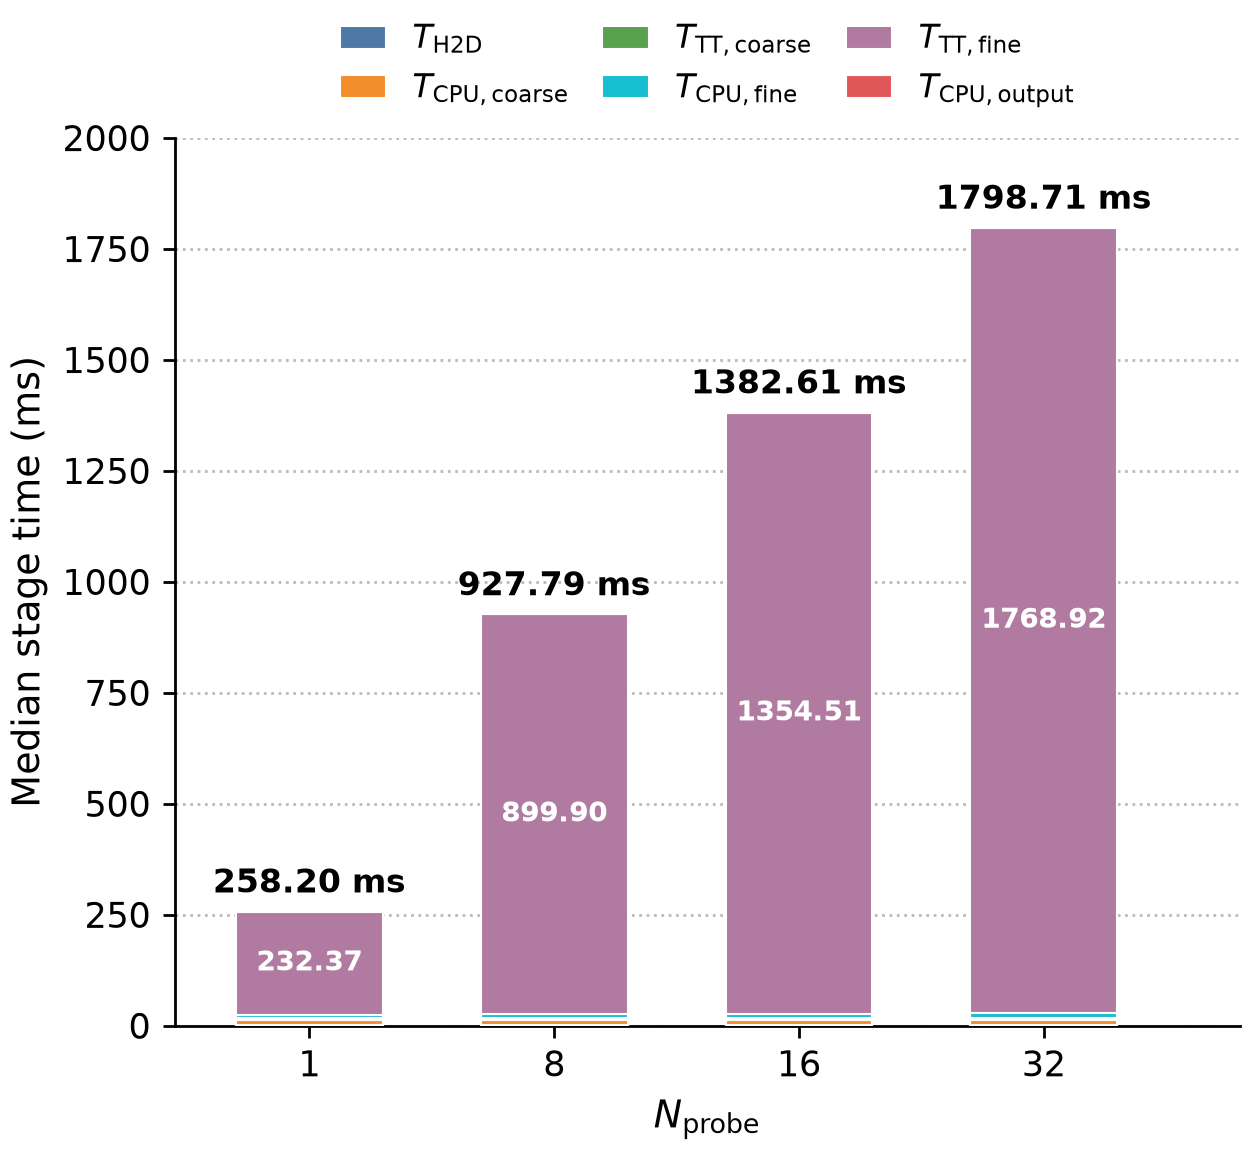
\includegraphics[width=\textwidth]
{./assets/memcopy_cost_nlist512.png}
\caption{Median Tenstorrent stage times for \(N_{\mathrm{list}}=512\),
including TT fine search.}
\label{fig:tt-stage-full}
\end{minipage}
\hfill
\begin{minipage}[t]{0.49\textwidth}
\centering
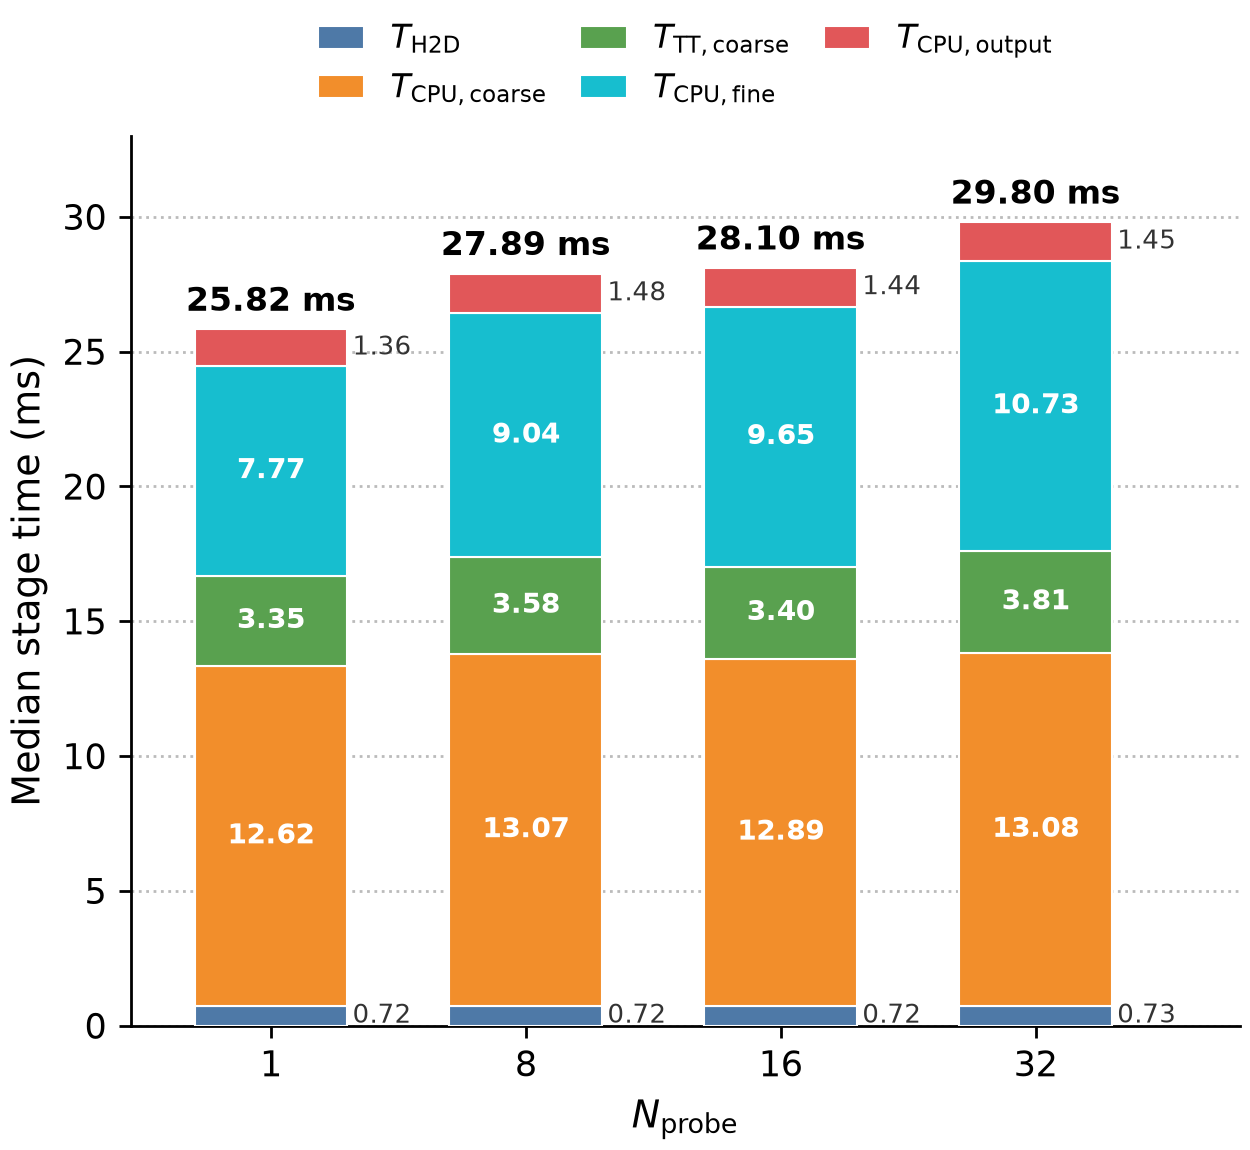
\includegraphics[width=\textwidth]
{./assets/memcopy_cost_nlist512_without_tt_fine.png}
\caption{Rescaled view of the same stage times with TT fine search omitted.}
\label{fig:tt-stage-detail}
\end{minipage}
\end{figure}

TT fine search dominates. As \(N_{\mathrm{probe}}\) increases from 1 to 32, the
total rises from 258.20 to 1,798.71~ms and fine search from 232.37 to
1,768.92~ms, accounting for 90.0\%, 97.0\%, 98.0\%, and 98.3\% of the four
totals. The totals agree with the independent throughput measurements: 1,798.71~ms
per 10,000 queries corresponds to about 5,560~QPS, against a median of 5,550~QPS.
All other stages together grow only from 25.82 to 29.80~ms: CPU coarse
configuration stays between 12.62 and 13.08~ms, TT coarse search between 3.35
and 3.81~ms, and CPU fine preparation grows from 7.77 to 10.73~ms. Optimizing
these stages would therefore have little effect at this \(N_{\mathrm{list}}\).
Host timing cannot tell whether compute, DRAM traffic, NoC communication,
circular-buffer backpressure, or synchronization limits the fine stage, which
motivates the device trace below.

\subsection{Device-Kernel Timeline}
\label{subsec:tt-device-timeline-results}

Figure~\ref{fig:tt-fine-pipeline-zoom} shows a device-profiler capture with
\(N_{\mathrm{list}}=512\) and \(N_{\mathrm{probe}}=8\), which reaches 85.8\%
recall, zoomed into the last three measured batches, labeled B1 to B3. It
covers the aggregation core and three consecutive fine-search workers. The
workers were taken in coordinate order, not selected by behavior, so the
figure is illustrative rather than a statistical sample of all workers. The
figure separates each core into its reader (NCRISC) and its three
compute threads (TRISC unpack, math, and pack). Each
worker scope is labeled with its batch and list task, so a bar covers the
processing of one task: a complete list or a chunk of at most 128 pages.

\begin{figure}[htbp]
\centering
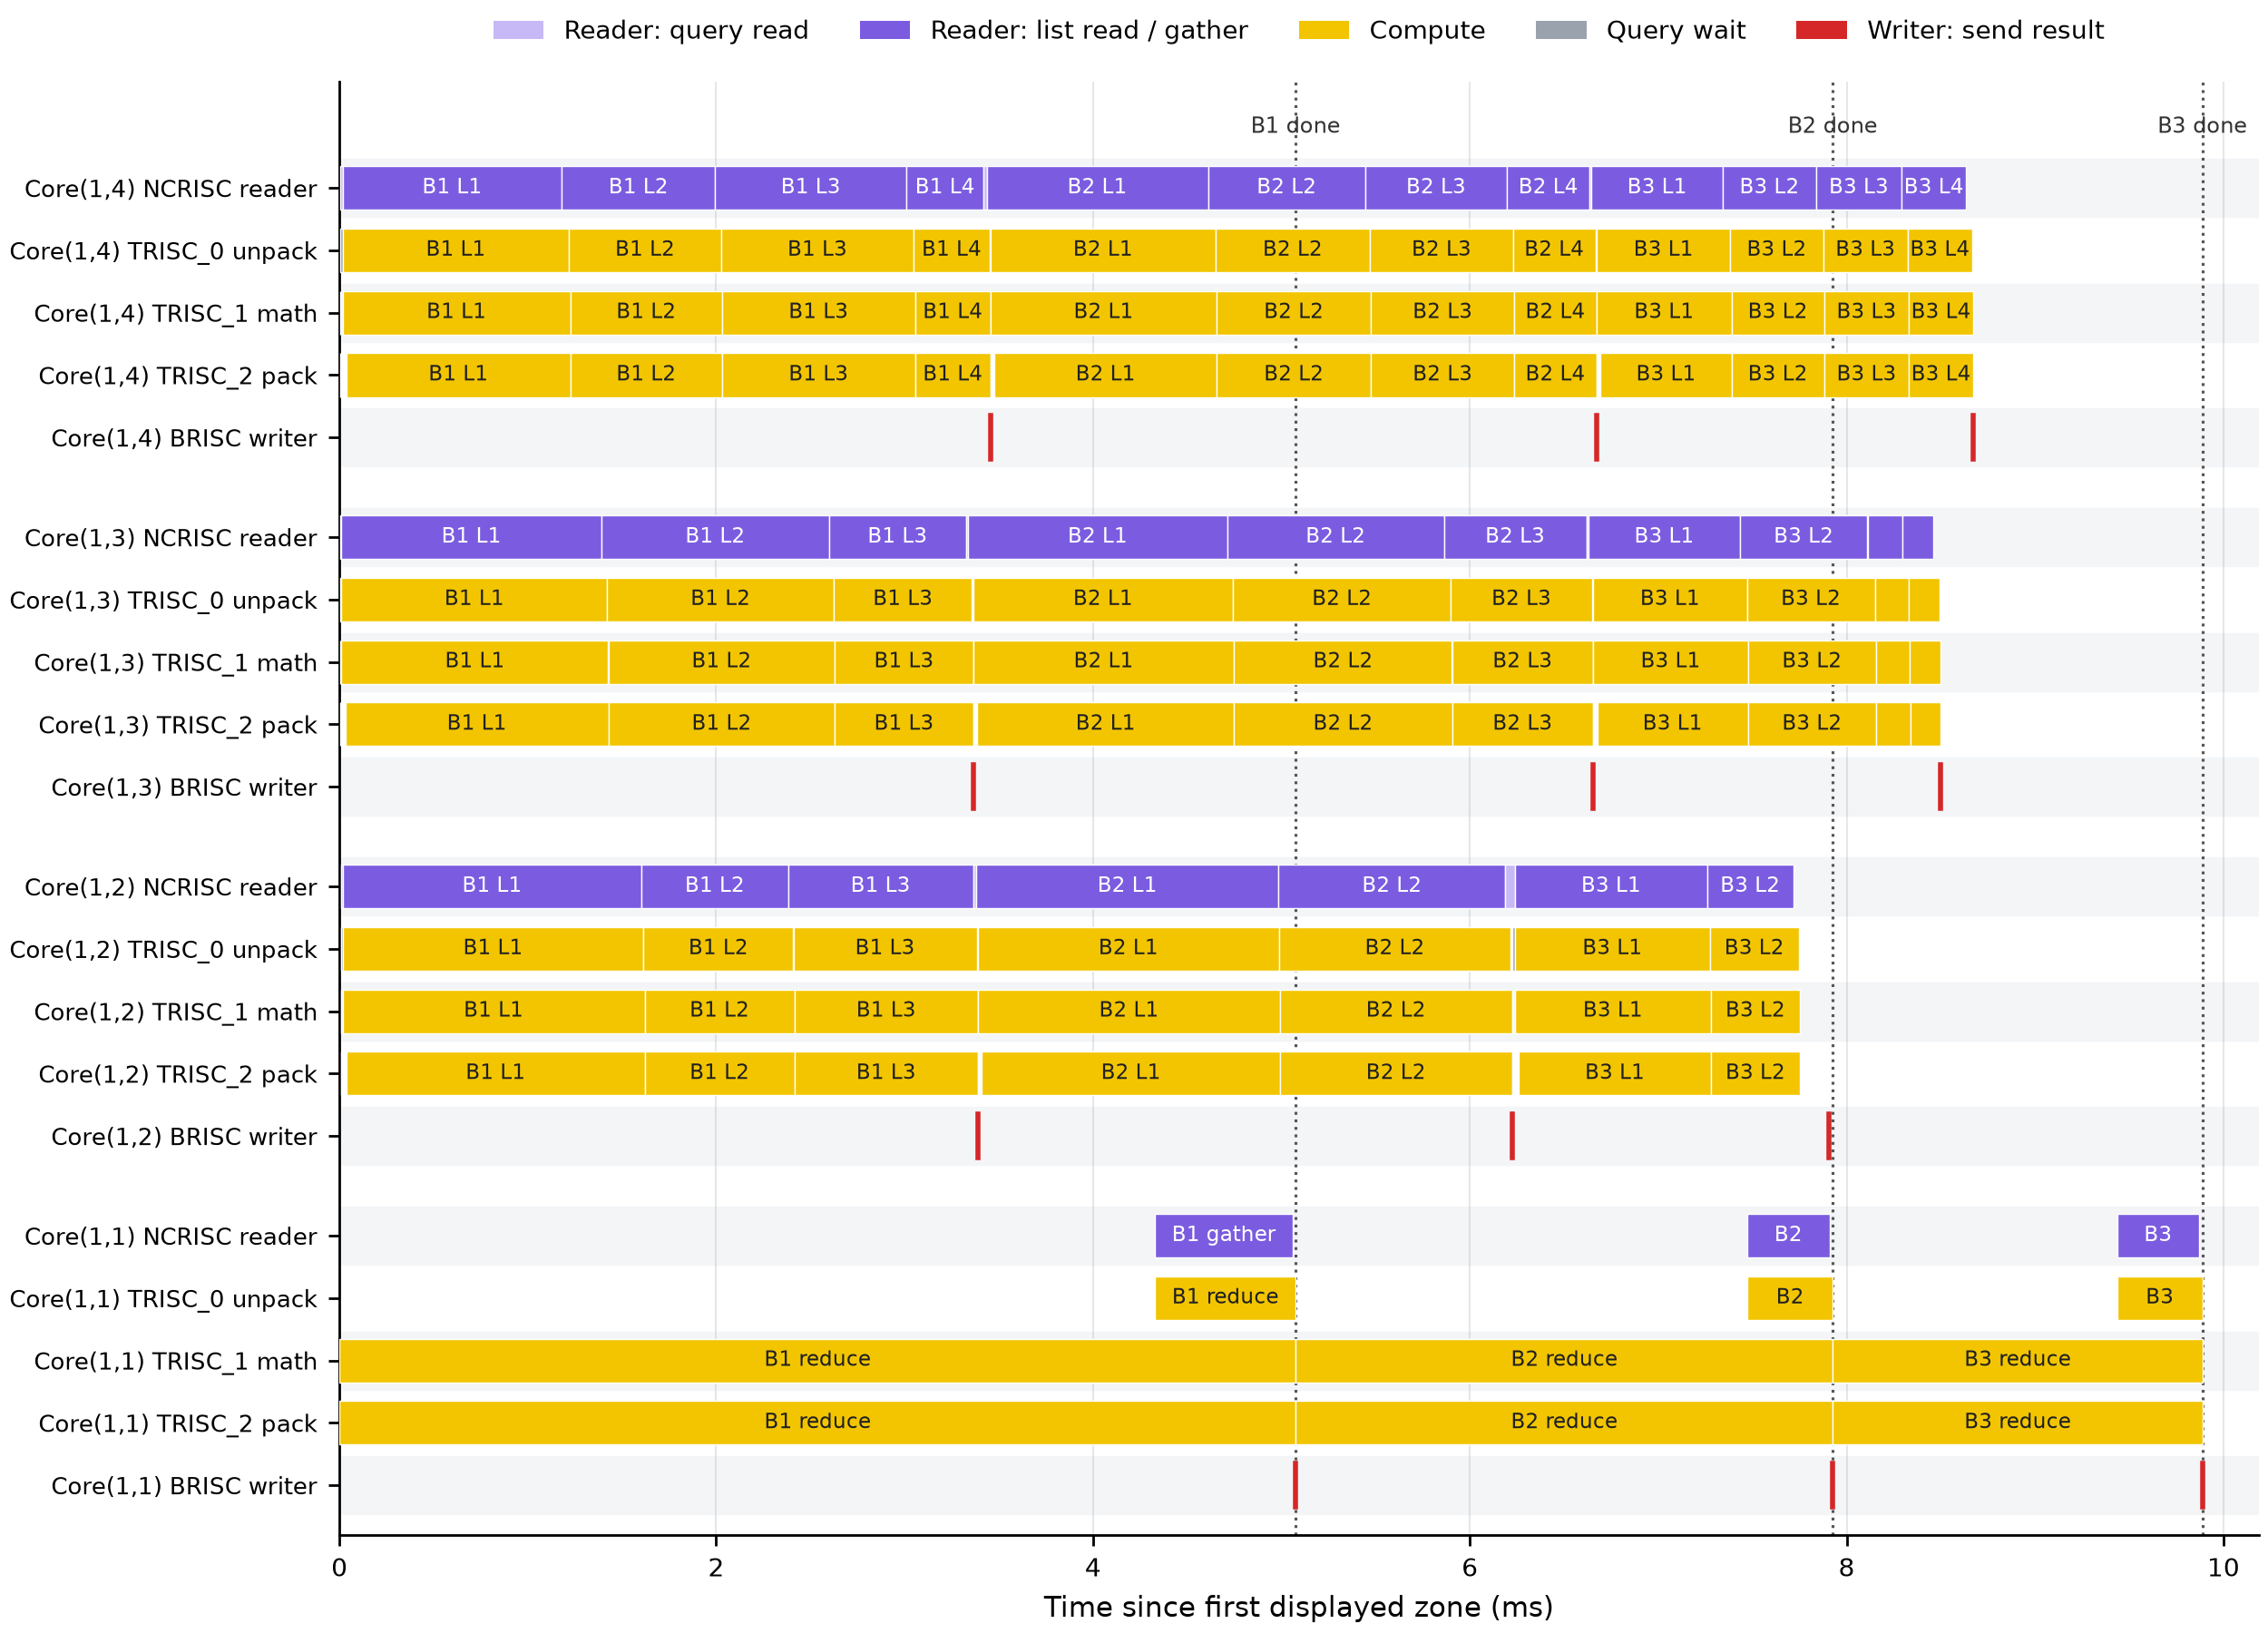
\includegraphics[width=\textwidth,keepaspectratio]
{./assets/fine_pipeline_horizontal.png}
\caption{Zoomed fine-search pipeline at
\((N_{\mathrm{list}},N_{\mathrm{probe}})=(512,8)\) for the last three 32-query
batches (B1 to B3), with one row per RISC processor of the aggregation core
(profiler core \((1,1)\)) and of three workers (profiler cores \((1,2)\) to
\((1,4)\)). A worker zone labeled B\(b\) L\(i\) covers the \(i\)-th list
task of batch \(b\); red ticks mark the writer sending a result, and dotted
lines mark the completion of each batch on the aggregation core.}
\label{fig:tt-fine-pipeline-zoom}
\end{figure}

Four observations follow from the zoomed trace.

\begin{enumerate}
    \item \textbf{Workers do not stop between batches.} Each worker starts the
    first list of the next batch within a few tens of microseconds of finishing
    the previous one. The aggregation core gathers B1 between about 4.3 and
    5.1~ms, when the three workers shown are already processing B2. Batch
    reduction is therefore off the workers' critical path and introduces no
    per-batch barrier.
    \item \textbf{Reader and compute advance in lock-step.} On every worker,
    each reader scope ends a few tens of microseconds before the corresponding
    compute scope, and the unpack, math, and pack scopes coincide. The
    pipeline overlaps the reading and scoring of the same list, and its fill
    latency at the start of a batch is only about 30--40~\(\mu\)s. Because each
    scope spans a whole task, the trace still cannot tell whether compute
    waits for data or the reader is throttled by full circular buffers.
    \item \textbf{Worker imbalance sets batch completion.} The three workers
    finish B1 within about 0.1~ms of each other, but drift apart later,
    completing B3 at about 7.8, 8.5, and 8.7~ms. The aggregator's B1 gather
    starts about 0.9~ms after the last of the three workers shown has finished
    B1, which is consistent with other workers finishing later. As batch
    completion depends on the slowest of the 63 workers, the greedy
    assignment of coarse list tasks translates directly into idle
    capacity.
    \item \textbf{Aggregation is short and overlapped.} The aggregator's
    gather and unpack scopes last about 0.73, 0.44, and 0.44~ms for the three
    batches. Its math and pack scopes span almost the entire interval because
    they include waiting for worker results, not because reduction is
    expensive. At this configuration the aggregation is therefore not an
    issue, but at low \(N_{\mathrm{probe}}\), where the workers finish a
    batch faster, the same per-batch cost becomes a likely bottleneck
    (Section~\ref{sec:nlist-nprobe-results}).
\end{enumerate}

The 2.85~ms between the completions of B1 and B2 matches the 2.96~ms per
batch measured by the stage timing at this configuration (927.79~ms over 313
batches), so the zoomed batches are representative. Batch B3 is visibly shorter on all workers because it is the final batch of
the repetition, which holds only 16 valid queries
(Equation~\ref{eq:tt-batches-per-repetition}) and therefore a smaller list
union. Each worker's writer sends its fixed-size local result in under
1~\(\mu\)s per batch, shown as red ticks.

Overall, the zoomed trace shows that fine-search time is spent inside the
per-list reader--compute loop of each worker and is extended by imbalance
across workers, whereas batch transitions and aggregation contribute little.

\paragraph{Single-list zoom.}
Figure~\ref{fig:tt-fine-cluster-bubbles} zooms further, into the processing of
16 consecutive pages (P0 to P15) of one inverted list on worker \((1,2)\),
captured with
\(N_{\mathrm{list}}=512\) and \(N_{\mathrm{probe}}=1\). Reader zones cover the
DRAM fetch of each page, and compute zones cover the unpacking, scoring, and
top-\(k\) update of each page.

\begin{figure}[htbp]
\centering
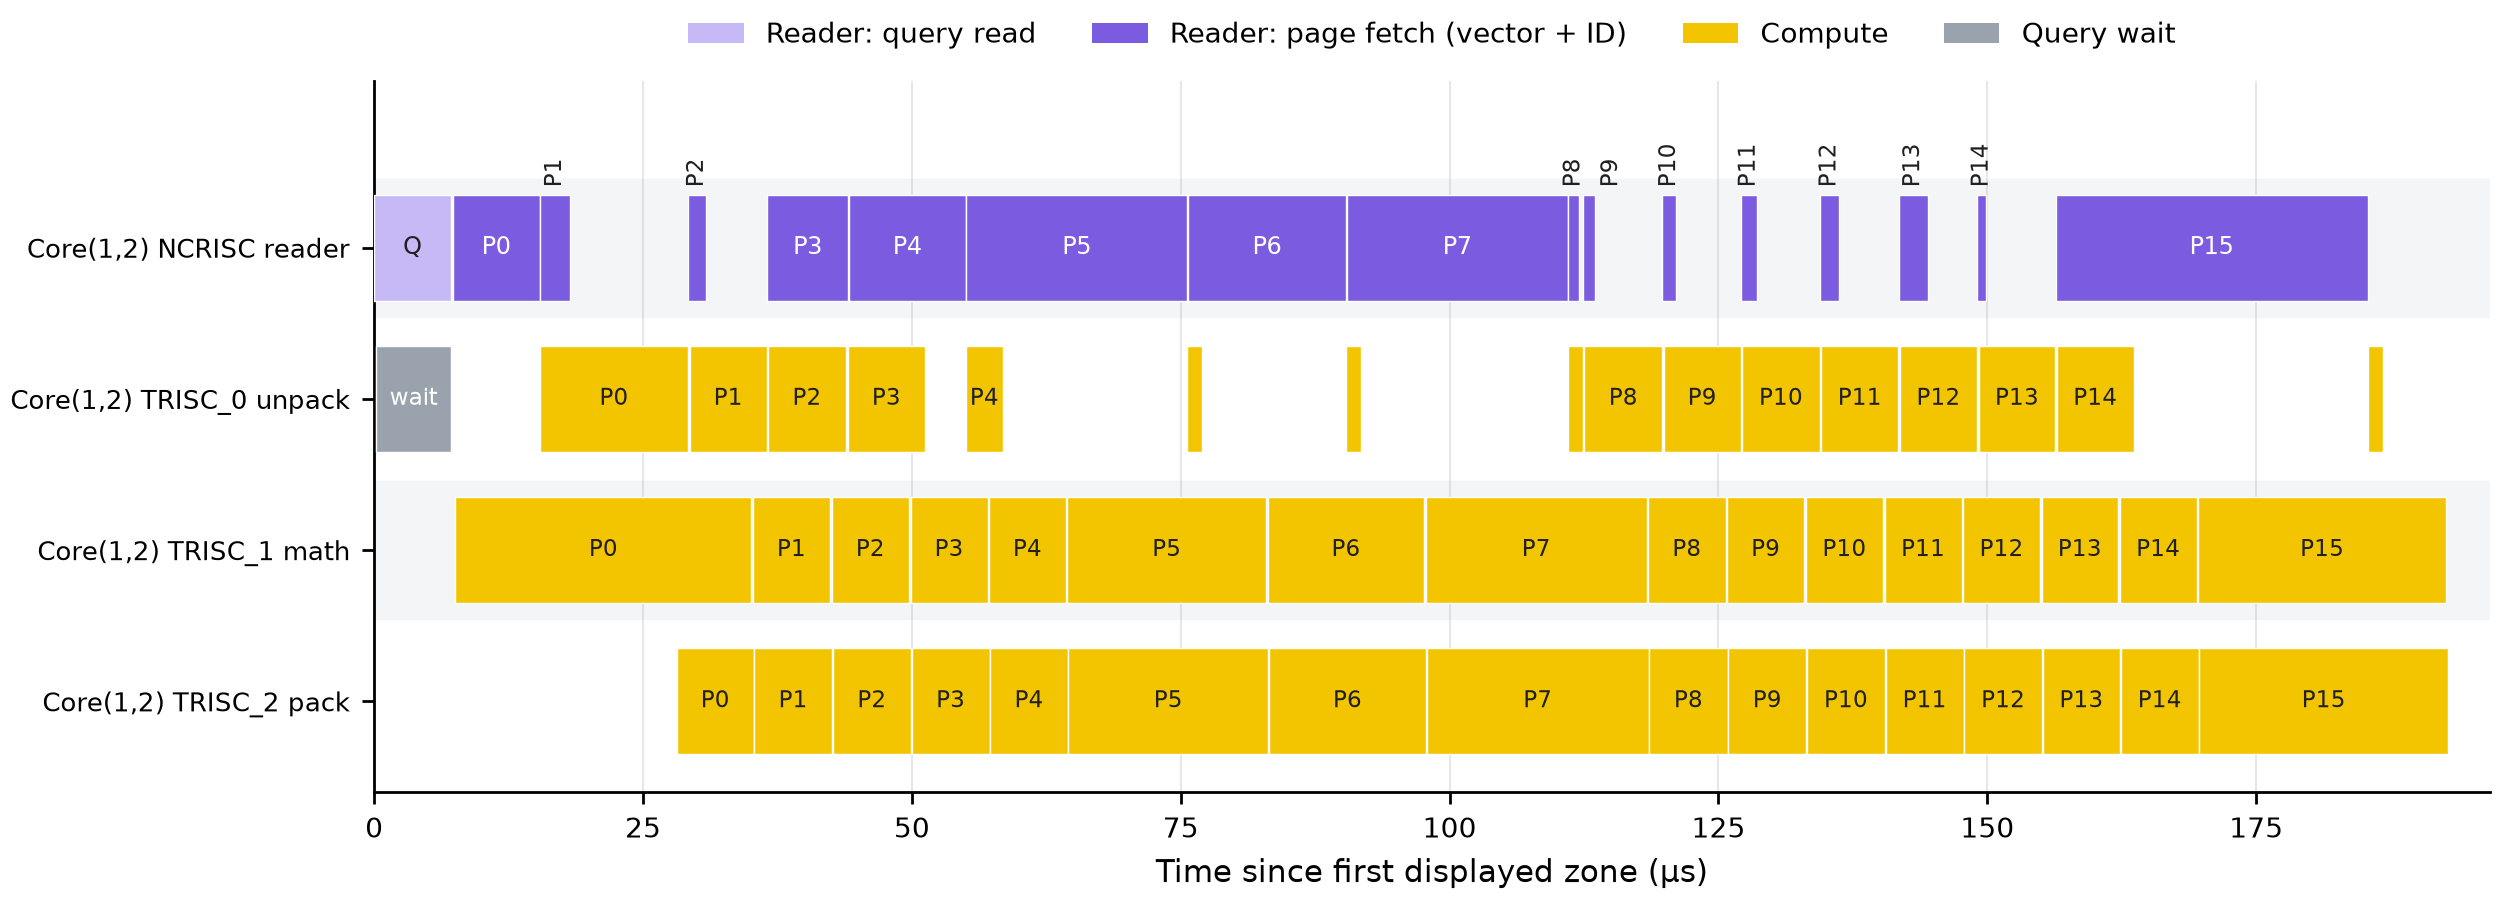
\includegraphics[width=\textwidth,keepaspectratio]
{./assets/fine_cluster_bubbles.png}
\caption{Processing of 16 consecutive pages (P0 to P15) of one inverted list on worker
\((1,2)\) at \((N_{\mathrm{list}},N_{\mathrm{probe}})=(512,1)\). The reader row
shows the query fetch and the DRAM fetch of each page; the compute rows show
the work on each page and the initial wait for the query.}
\label{fig:tt-fine-cluster-bubbles}
\end{figure}

\begin{enumerate}
    \item \textbf{Compute costs about 7~\(\mu\)s per page.} When data is
    available (P1 to P4 and P8 to P14), each page occupies the math and pack
    threads for about 7~\(\mu\)s, while the reader fetches the next
    page mostly in under 3~\(\mu\)s shortly before it is needed. In this regime
    the pipeline is limited by the per-page compute step, not by arithmetic
    (see below), and the reader waits for free buffer space. A
    page requires only four \(32\times32\) tile multiplications, so the
    7~\(\mu\)s suggests that most of the compute time is spent outside the
    matrix multiplication, in the top-\(k\) update.
    \item \textbf{Slow fetches create bubbles.} The fetches of P5, P6, P7, and
    P15 take 15--29~\(\mu\)s instead of under 3~\(\mu\)s. The unpacker then has no
    input, and the math and pack zones of these pages stretch to
    15--23~\(\mu\)s. Start-up adds a further bubble: the query fetch and the
    first page read delay the pack thread until about 28~\(\mu\)s, and the
    first page is complete only at about 35~\(\mu\)s.
    \item \textbf{About 40\% of the time is waiting.} Sixteen pages at
    about 7~\(\mu\)s account for roughly 115~\(\mu\)s of the 193~\(\mu\)s
    shown, so compute waits for data for about 40\% of the time.
    \item \textbf{The buffer hides little variation.} The reader runs only
    about one page ahead of compute, as expected from the double-buffered
    candidate buffers (Section~\ref{subsec:fine-worker-pipeline}), so a
    single slow fetch stalls the
    pipeline immediately, whereas the 8--11~\(\mu\)s fetches of P3 and P4 are
    hidden because they start early enough. Deeper buffering does not solve
    this, however: in single exploratory runs at \((512,32)\) with an
    instrumented build, letting the reader prefetch eight pages instead of two
    made fine search about 7\% slower (2,006 against 1,880~ms per 10,000
    queries), consistent with the additional outstanding reads adding to the
    contention between workers for the DRAM channels.
\end{enumerate}

\paragraph{Arithmetic intensity.} The ``compute'' in the trace is not
arithmetic. Each page fetches 12,288~bytes, 8,192 for the 32 vectors of 128
FP16 dimensions and 4,096 for the identifier tile, and performs one
\(32\times128\) by \(128\times32\) multiplication of 262,144 floating-point
operations. Even with all 32 query rows in use, this is only 21~operations per
byte, an order of magnitude below the balance point of the Wormhole n150, about
257~operations per byte for its 74~FP16 TFLOP/s and 288~GB/s
\cite{tenstorrent_wormhole_spec}. Most rows are not even useful: only the
queries that selected the list need its scores, which on average is one row
in 12 to 31 (Table~\ref{tab:union-scan}), so the useful intensity is only
0.7--1.7~operations per byte. The fine search is therefore memory-bound in the
roofline sense, and the matrix engine is never its limit: at \((512,32)\) it
runs at about 1.4~TFLOP/s, 2\% of the peak. The DRAM is not saturated either,
since the 9.5~million pages fetched in 1.77~s amount to about 66~GB/s, 23\% of
the peak bandwidth. The time per page is set instead by the work around the
multiplication, chiefly the top-\(k\) update of the scores and identifiers, and
by the latency of the fetches, which become slow and irregular when many
workers read at the same time. Both depend on the number of pages processed,
which is why reducing that number matters more than faster arithmetic.

\paragraph{Growth with \(N_{\mathrm{probe}}\).}
The window was captured at \(N_{\mathrm{probe}}=1\), which is the most
favorable case for data availability: the union of a 32-query batch then
contains at most 32 lists, so at most 32 of the 63 workers are active. Three
effects are expected to enlarge the problem as \(N_{\mathrm{probe}}\) grows.
\begin{enumerate}
    \item \textbf{More concurrent readers.} From \(N_{\mathrm{probe}}=2\)
    onwards, the union can exceed the 63 workers, so all of them fetch pages
    at the same time and compete for the same DRAM channels and NoC links.
    The trace does not show why the fetches of P5 to P7 and P15 are slow, but
    if contention is the cause, such fetches become more frequent and longer.
    \item \textbf{More pages per worker.} Each worker processes more list
    tasks per batch, so every stall is repeated over more pages. Even at an
    unchanged fraction of waiting per page, the absolute waiting time grows
    with the number of pages scanned.
    \item \textbf{Constant compute cost per page.} The approximately
    7~\(\mu\)s per page does not decrease with \(N_{\mathrm{probe}}\), so the
    phases limited by the per-page compute step also grow in proportion to
    the pages scanned.
\end{enumerate}
Consistently with these effects, TT fine search grows from 232 to
1,769~ms per 10,000 queries between \(N_{\mathrm{probe}}=1\) and 32
(Section~\ref{sec:tt-stage-results}).
Reducing the data fetched per query and the cost of the per-page top-\(k\)
update are the two main directions for improving fine search.

\section{Workload Energy}
\label{sec:energy-results}

Table~\ref{tab:energy-recall} and Figure~\ref{fig:query-energy} report the
median energy of ten complete 100,000-query sessions at each recall-matched
point, amortized per query with Equation~\ref{eq:energy-per-query}, together
with the interquartile range (IQR) and the relative standard deviation (RSD)
across the ten sessions. For Tenstorrent, the energy is that of the complete
system, device and host together.

\begin{table}[htbp]
\centering
\caption{Workload energy for 100,000-query sessions, including
initialization. Energy is the median of ten sessions, with the IQR and RSD
across them, and its amortized per-query value. Configuration denotes
\((N_{\mathrm{list}},N_{\mathrm{probe}})\).}
\label{tab:energy-recall}
\small
\setlength{\tabcolsep}{2.4pt}
\renewcommand{\arraystretch}{1.08}
\begin{tabular}{lrrrrrr}
\toprule
Architecture & Config. & Recall@10 & Energy (J) & IQR (J) & RSD & mJ/query \\
\midrule
CPU (56 cores)  & \((2048,4)\)  & 60.46\% & 6,995.69  & 6,927--7,090   & 2.36\% & 69.957 \\
                & \((2048,16)\) & 78.33\% & 7,981.57  & 7,901--8,070   & 1.93\% & 79.816 \\
                & \((1024,32)\) & 88.49\% & 9,211.55  & 9,140--9,351   & 1.40\% & 92.116 \\
                & \((512,64)\)  & 95.54\% & 21,872.36 & 21,831--21,988 & 0.67\% & 218.724 \\
\midrule
CPU (112 cores) & \((2048,4)\)  & 60.46\% & 6,915.42  & 6,835--7,002   & 2.65\% & 69.154 \\
                & \((2048,16)\) & 78.33\% & 7,526.78  & 7,467--7,747   & 2.67\% & 75.268 \\
                & \((1024,32)\) & 88.49\% & 7,292.36  & 7,270--7,371   & 1.50\% & 72.924 \\
                & \((512,64)\)  & 95.54\% & 14,928.76 & 14,741--15,060 & 1.46\% & 149.288 \\
\midrule
GPU (A100) + CPU & \((2048,4)\)  & 60.47\% & 932.97   & 776--1,085   & 36.60\% & 9.330 \\
                 & \((2048,16)\) & 78.33\% & 940.54   & 847--1,019   & 24.01\% & 9.405 \\
                 & \((1024,32)\) & 88.49\% & 1,064.14 & 1,021--1,113 & 5.72\%  & 10.641 \\
                 & \((512,64)\)  & 95.53\% & 2,010.66 & 1,989--2,131 & 6.23\%  & 20.107 \\
\midrule
TT + CPU         & \((2048,4)\)  & 62.24\% & 3,050.09 & 3,036--3,076 & 1.78\% & 30.501 \\
                 & \((2048,12)\) & 79.16\% & 3,542.92 & 3,525--3,562 & 3.85\% & 35.429 \\
                 & \((1024,16)\) & 88.03\% & 3,438.38 & 3,420--3,457 & 1.32\% & 34.384 \\
                 & \((512,32)\)  & 95.37\% & 4,692.64 & 4,669--4,741 & 1.93\% & 46.926 \\
\bottomrule
\end{tabular}
\end{table}

\begin{figure}[htbp]
\centering
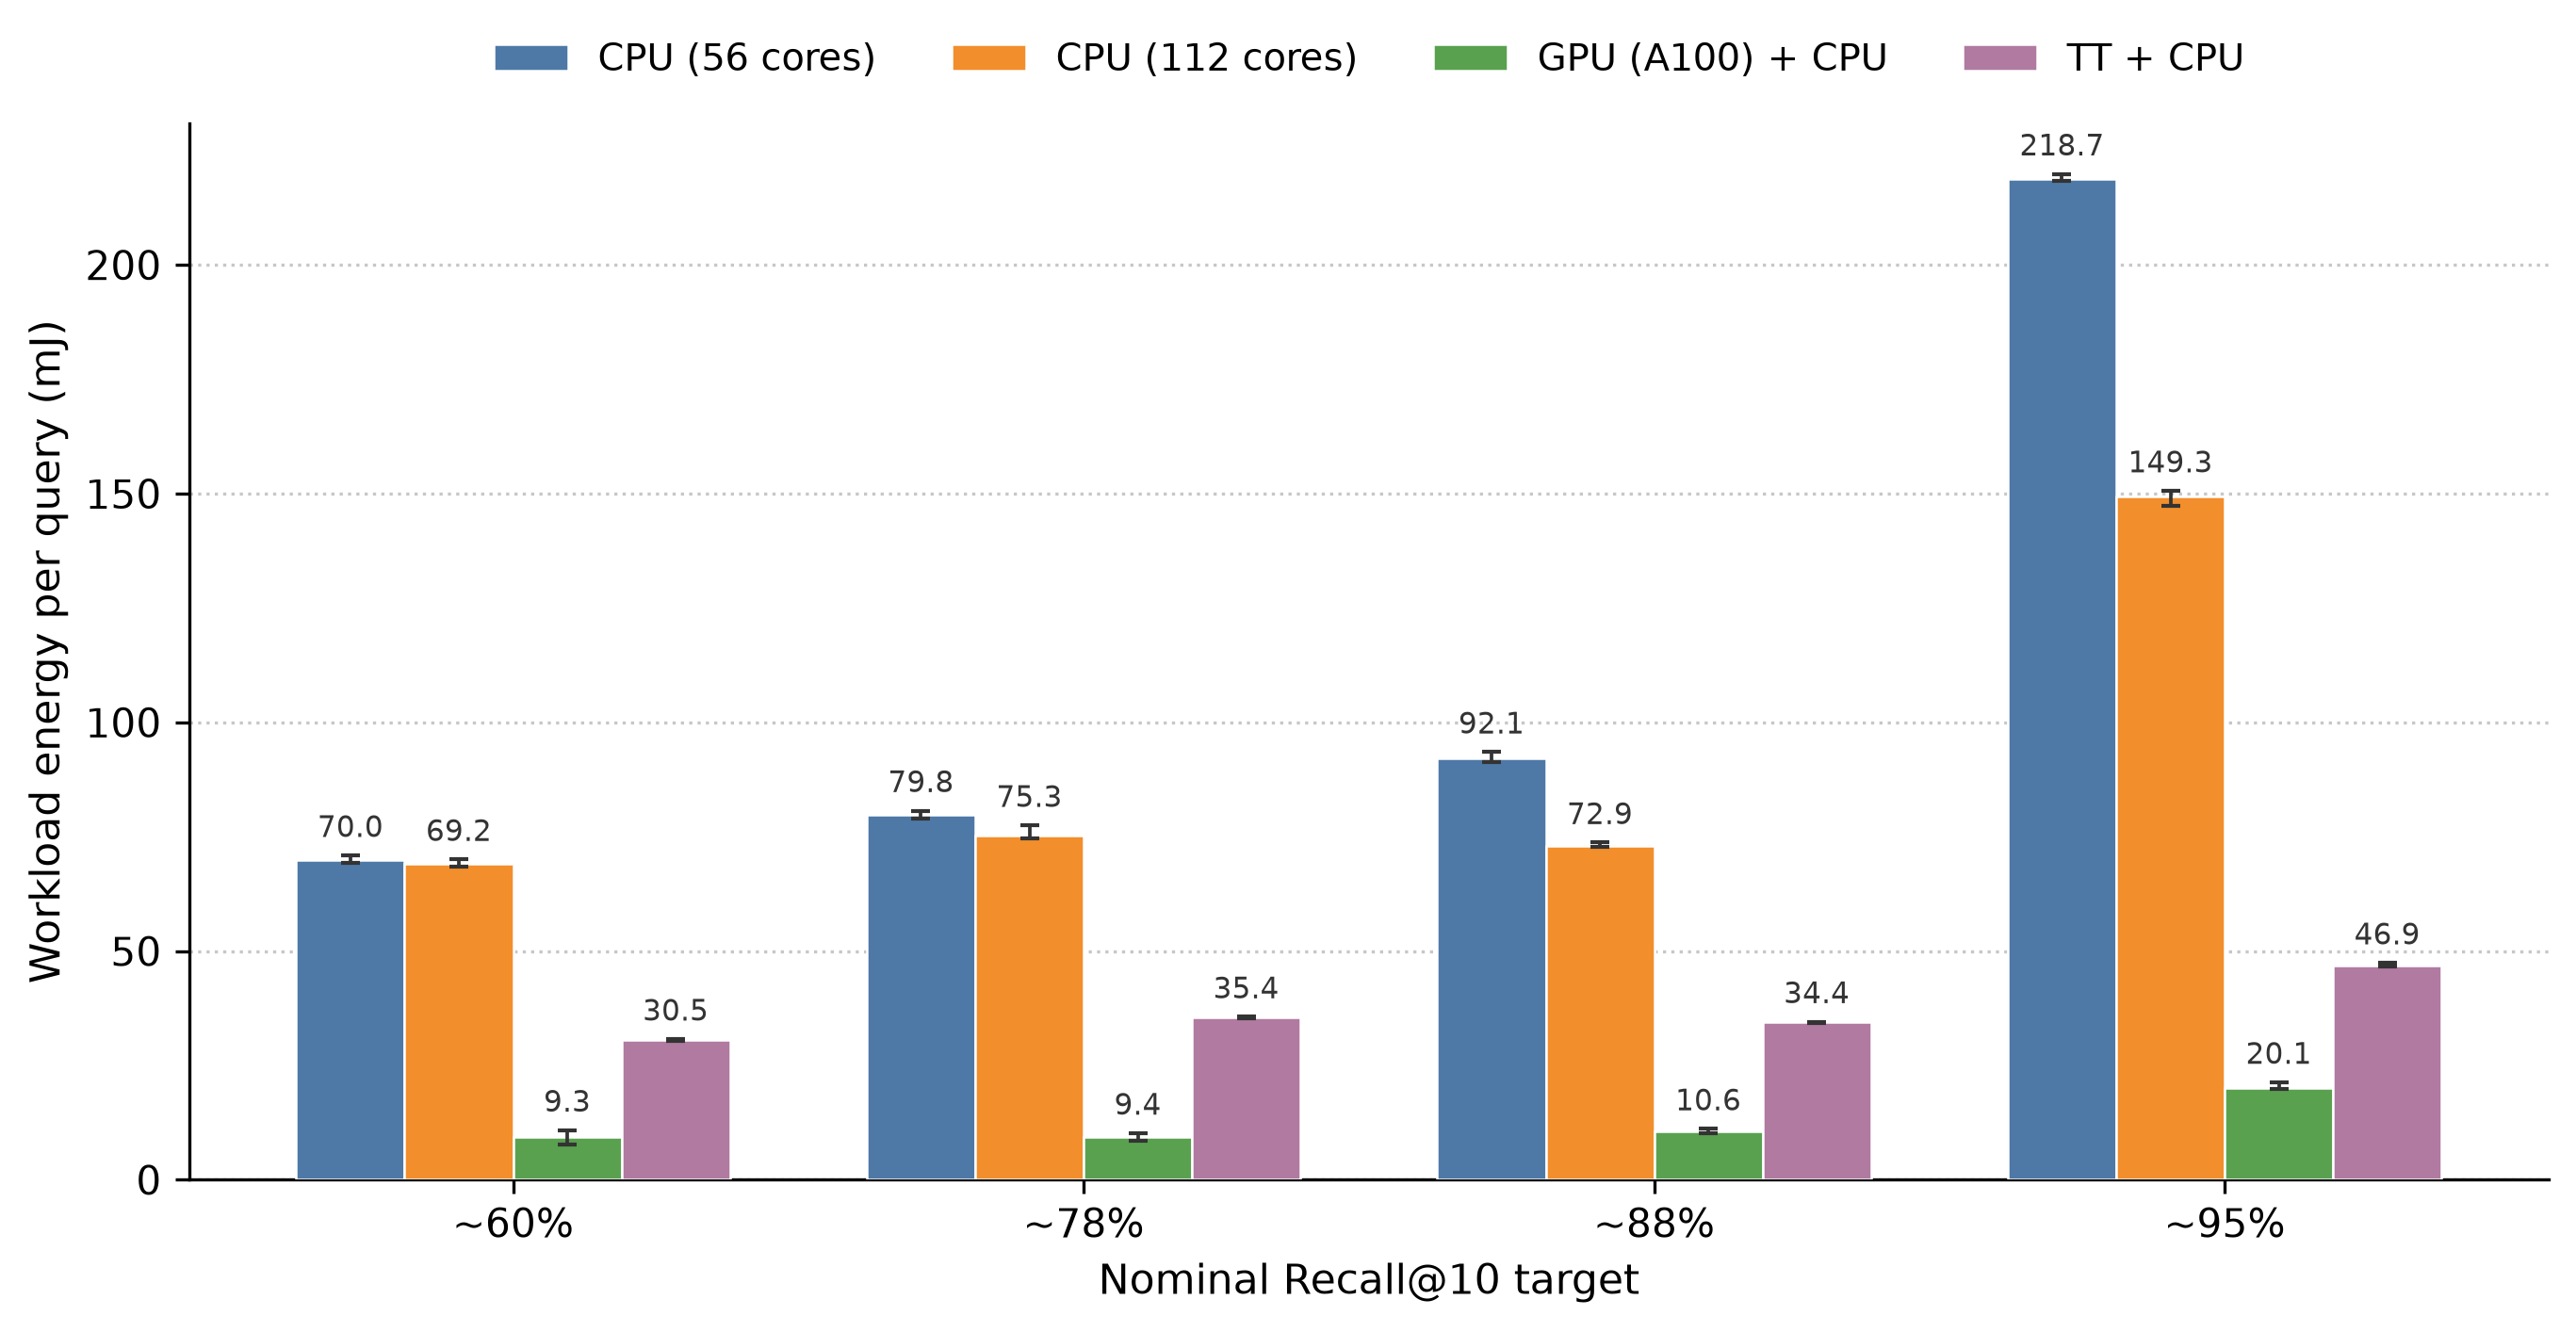
\includegraphics[width=0.96\textwidth]{./assets/energy_per_query_recall.png}
\caption{Amortized workload energy per query at approximately matched
Recall@10, including initialization. Bars show the median of ten sessions and
whiskers the interquartile range.}
\label{fig:query-energy}
\end{figure}

The GPU system uses the least energy at every target, 9.3--20.1~mJ per query.
Tenstorrent is second, with 30.5--46.9~mJ per query, which is 2.3 times the
GPU value at the 95\% target and 3.2--3.8 times at the lower targets. Both CPU
configurations use the most: 69--92~mJ per query up to the 88\% target and
149--219~mJ at 95\%. Tenstorrent therefore uses 53--63\% less energy than the
CPUs up to the 88\% target, and 78.5\% and 68.6\% less than the 56-core and
112-core CPUs at 95\%, where the GPU uses 90.8\% and 86.5\% less.

The CPU and Tenstorrent values are reproducible across sessions, with an RSD
of at most 2.67\% on the CPUs and 3.85\% on Tenstorrent. The GPU values vary more at low recall,
with an RSD of 36.6\% at 60\% and 24.0\% at 78\%, because these sessions last
less than 3~s and are almost entirely initialization; at the 88\% and 95\%
targets the RSD is about 6\%.

\paragraph{The host dominates Tenstorrent's energy.}
The Wormhole device itself uses 327--850~J per session, 23.9--33.6~W on
average, or only 10.7--18.1\% of the system energy. The remaining 152--200~W is
drawn by the dual-socket EPYC 7301 host, whose combined rated TDP of about
310--340~W is less than half that of the 700~W CPU node. The energy of the
Tenstorrent system is therefore set mainly by its host.

For a device-to-device view at the 95\% target, the A100 board trace of one
session is examined on its own; the board power is integrated in every GPU
session, but only this trace is analyzed separately here. The board draws about 66~W when idle and about 377~W
on average while searching, with a peak of 386~W, below its 550~W limit; the
high-power interval lasts 2.2~s, matching the 2.31~s search time. Over the
session the board uses 1,066~J, or 10.7~mJ per query, against 8.5~mJ for the
Wormhole chip. The two devices therefore use comparable energy for this
workload, keeping in mind that the chip telemetry of the Wormhole excludes the
board-level losses that the A100 measurement includes: the A100 draws far more
power, but finishes the search about 7.8 times faster.

The GPU system is not dominated by its host to the same extent. At the 95\%
target, the 1,066~J of the A100 board are about half of the 2,011~J median
energy of the complete A100 system, whereas the Wormhole chip accounts for only
18\% of the Tenstorrent system. Since the board figure comes from a single
session and the system figure is a median over ten, this split is approximate,
but it shows that the energy gap between the two systems lies mainly in their
host energy rather than in the accelerators. The Tenstorrent host is not more
power-hungry, drawing 152~W at this target against about 218~W for the A100
host, but it is powered for a session 5.8 times longer. The Wormhole device
thus reaches a device energy comparable to that of the A100 while being a
lower-cost accelerator, and shortening the session, through faster
initialization and search, is the most direct way to reduce the energy of the
Tenstorrent system.

\paragraph{Initialization dominates at low recall.}
Table~\ref{tab:energy-session-composition} relates each session to its search
time, estimated as \(Q_{\mathrm{run}}/\operatorname{QPS}_{\mathrm{reported}}\).
At the 60\% target, search occupies only 2--4\% of every CPU and GPU session
and 15\% of the Tenstorrent session; the remainder is process start-up,
dataset loading, list assignment, and, on the accelerators, device setup and
index transfer. The per-query values in
Table~\ref{tab:energy-recall} therefore measure the cost of a complete
100,000-query job from a cold start, not the energy of search alone.

The time spent outside search differs strongly between the platforms. On the
GPU system it is 2.0--2.8~s for every configuration. On the CPUs it grows with
\(N_{\mathrm{list}}\), from 3.0--7.2~s at 512 lists to 9.3--10.8~s at 1024 and
17.4--17.9~s at 2048, and at 1024 and 2048 lists it is almost the same on 56
and 112 cores. On
Tenstorrent, whose host also performs the assignment, it grows from 7.3~s at
512 lists to 8.2~s at 1024 and 11.6--11.7~s at 2048. This is consistent with
the assignment of the 1.18 million database vectors to their nearest
centroids, whose cost is proportional to \(N_{\mathrm{list}}\), running on the
host CPU without benefiting from additional cores, whereas the GPU performs it
on the device. The low-recall CPU and Tenstorrent energy is therefore
dominated by initialization rather than by search.

\begin{table}[htbp]
\centering
\caption{Composition of the energy sessions. Search time is
\(100{,}000/\operatorname{QPS}_{\mathrm{reported}}\); session time is the
median duration of the complete session, which includes the search; and
average power is the median workload energy divided by the median session
time.}
\label{tab:energy-session-composition}
\small
\setlength{\tabcolsep}{4pt}
\renewcommand{\arraystretch}{1.08}
\begin{tabular}{lrrrrr}
\toprule
Architecture & Target & Search (s) & Session (s) & Search share & Avg.\ power (W) \\
\midrule
CPU (56 cores)   & 60\% & 0.66  & 18.171 & 3.6\%  & 385.0 \\
                 & 78\% & 2.28  & 19.667 & 11.6\% & 405.8 \\
                 & 88\% & 8.72  & 17.983 & 48.5\% & 512.2 \\
                 & 95\% & 31.35 & 34.376 & 91.2\% & 636.3 \\
\midrule
CPU (112 cores)  & 60\% & 0.38  & 18.211 & 2.1\%  & 379.7 \\
                 & 78\% & 1.25  & 19.126 & 6.5\%  & 393.5 \\
                 & 88\% & 4.53  & 15.314 & 29.6\% & 476.2 \\
                 & 95\% & 17.18 & 24.395 & 70.4\% & 612.0 \\
\midrule
GPU (A100) + CPU & 60\% & 0.06  & 2.828  & 2.2\%  & 329.9 \\
                 & 78\% & 0.18  & 2.795  & 6.6\%  & 336.5 \\
                 & 88\% & 0.62  & 2.862  & 21.7\% & 371.8 \\
                 & 95\% & 2.31  & 4.335  & 53.3\% & 463.8 \\
\midrule
TT + CPU         & 60\% & 2.01  & 13.626 & 14.8\% & 223.8 \\
                 & 78\% & 4.56  & 16.285 & 28.0\% & 217.6 \\
                 & 88\% & 9.29  & 17.486 & 53.1\% & 196.6 \\
                 & 95\% & 18.02 & 25.294 & 71.2\% & 185.5 \\
\bottomrule
\end{tabular}
\end{table}

\paragraph{More CPU cores do not cost more energy.}
The 56-core CPU never uses less energy than the 112-core CPU. At the 60\%
target the two are within 1.2\%, because both sessions are almost entirely
initialization, which does not benefit from more cores, so the node draws about 380~W in
either configuration. As search takes a larger share of the session, the
56-core CPU uses 6\% more energy at 78\%, 26\% more at 88\%, and 47\% more at
95\%. Doubling the cores does not double the power, because most of the node's
power is fixed: both sockets, with their caches, memory controllers, and idle
cores, are powered for the whole session regardless of how many cores search.
Moreover, with 56 cores the active cores can likely run at higher clock frequencies
and draw more power each, while the idle ones still draw some; with 112 cores
all of them are active, but each draws less, so the average power changes
little.
Assuming about 380~W during initialization, the average power during the
search at the 95\% target is roughly 660~W with 56 cores and 710~W with 112,
only about 7\% more, while the search takes 31.35~s instead of 17.18~s. The
112-core search therefore spends about 12~kJ instead of 21~kJ: it pays the
fixed power of the node for a much shorter time.

\subsection{Workload Throughput and Energy}
\label{sec:session-throughput-energy}

To view speed and energy on the same workload boundary,
Figure~\ref{fig:session-throughput-energy} uses the workload throughput
\begin{equation}
\Theta_{\mathrm{workload}}
=\frac{Q_{\mathrm{run}}}{t_{\mathrm{session}}}
=\frac{100{,}000}{t_{\mathrm{session}}},
\label{eq:session-throughput}
\end{equation}
which, unlike the search-only QPS of Section~\ref{sec:cross-platform-performance},
includes initialization.

\begin{figure}[htbp]
\centering
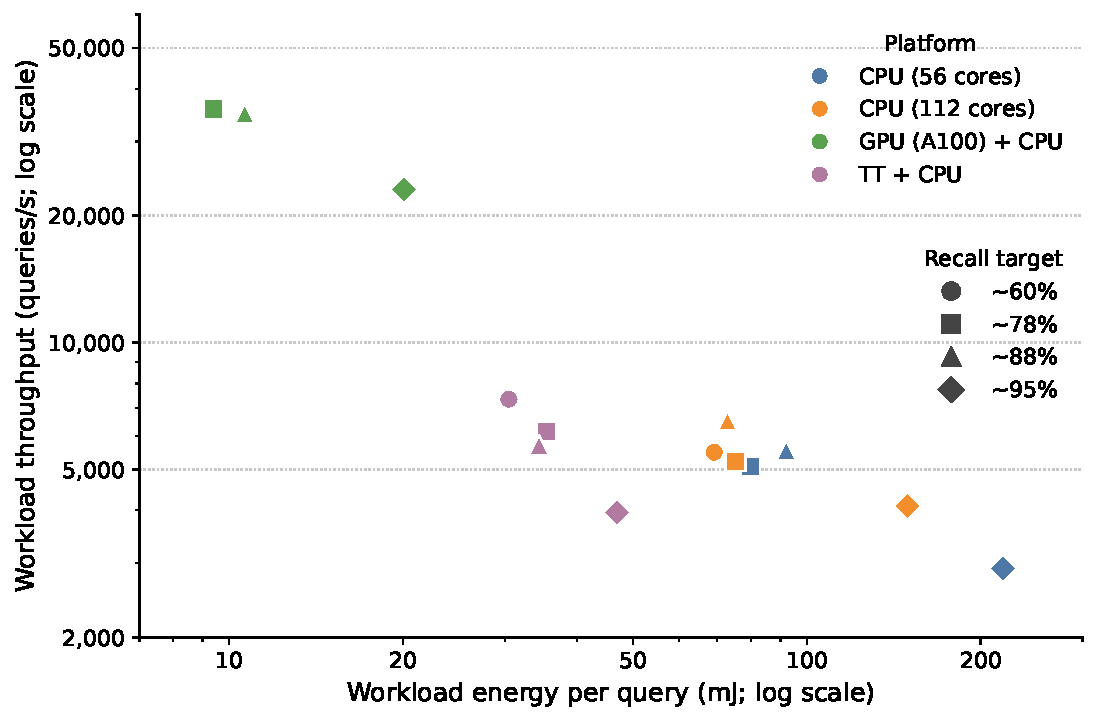
\includegraphics[width=0.94\textwidth]
{./assets/session_throughput_vs_energy.pdf}
\caption{Workload throughput, including initialization, versus amortized
workload energy per query at approximately matched Recall@10 targets.}
\label{fig:session-throughput-energy}
\end{figure}

The GPU system lies in the upper left at every target: it completes the
workload fastest, at 35,000--36,000 queries per second up to the 88\% target,
and uses the least energy. The Tenstorrent and CPU sessions reach similar
workload throughput, between about 2,900 and 7,300 queries per second, because
initialization takes a large part of each of them, but Tenstorrent uses
53--79\% less energy. At the 95\% target, the GPU, 112-core, Tenstorrent, and
56-core sessions correspond to 23,068, 4,099, 3,954, and 2,909 queries per
second. These ratios are smaller than the search-only differences in
Table~\ref{tab:qps-matched} because initialization occupies part of every
session.

\section{Summary of Results and Limitations}
\label{sec:results-summary}

The main observations are:
\begin{itemize}
    \item The GPU has the highest search throughput at every recall level, from
    31.9 times Tenstorrent at 60\% to 7.8 times at 95\%.
    \item Tenstorrent is slower than both CPU configurations up to about 88\%
    recall; at 95\% it is 1.74 times faster than the 56-core CPU and on par
    with the 112-core CPU against the evaluated Faiss grid.
    \item The batch-level union raises Tenstorrent recall by up to 7.5
    percentage points at equal parameters, but each query is scored against
    12--32 times as many vectors as in Faiss, and against 81.7\% of the
    database at the 95\% target. Consecutive queries share almost no lists. At low \(N_{\mathrm{probe}}\), Tenstorrent throughput is capped
    by a per-batch cost of about 0.58~ms.
    \item Fine search accounts for 90--98\% of the Tenstorrent search path at
    \(N_{\mathrm{list}}=512\). Inside it, reader and compute advance in
    lock-step on each list, batch transitions and aggregation are overlapped
    with worker execution, and batch completion is set by the slowest worker.
    Within a list, compute costs about 7~\(\mu\)s per page and waits for
    slow DRAM fetches for about 40\% of the time.
    \item The GPU system uses the least workload energy at every recall
    target, Tenstorrent 2.3--3.8 times as much, and the CPUs the most.
    Tenstorrent uses 53--79\% less energy than the CPUs, and its energy is
    dominated by its host, the device accounting for only 11--18\% of it. On
    the CPU node, 112 cores never use more energy than 56, because the node's
    power is drawn for the whole session and more cores finish sooner.
\end{itemize}

These results are subject to the following limitations:
\begin{itemize}
    \item \textbf{Workload boundary.} Energy includes initialization, so the
    per-query values depend on workload length and do not measure search
    energy alone.
    \item \textbf{Quality matching.} Tenstorrent and Faiss process different
    candidate sets, so cross-platform points are matched only approximately
    by recall, and the effect of alternative query groupings is not
    evaluated.
    \item \textbf{Platforms.} The three systems use different hosts and
    hardware generations, including a 2017 AMD EPYC 7301 host for
    Tenstorrent, and their device power sensors cover different parts of the
    accelerator (chip telemetry on Tenstorrent, the whole board on the A100).
    The comparison is between complete systems, not between processor
    architectures in isolation.
    \item \textbf{Dataset scale.} The 16-bit database occupies about 237~MB,
    which is small for a vector-search deployment and close to the combined
    last-level cache of the dual-socket CPU node. The dataset was chosen as a
    standard benchmark with published exact neighbors, which the
    recall-matched comparison requires. Collections of the size that
    motivates this work, such as large RAG corpora, would not fit on one
    device: in the current layout the 12~GB of the Wormhole n150 hold about
    30 million vectors (Section~\ref{sec:conclusion-limitations}); larger
    collections would require distributing the index over several devices or
    streaming lists from host memory, which are natural extensions of this
    work.
    \item \textbf{Bottleneck attribution.} The single-list trace covers 16
    pages of one list on one worker at \(N_{\mathrm{probe}}=1\). It separates fetch from compute
    but not the matrix multiplication from the top-\(k\) update, and it does
    not explain why some DRAM fetches are slow.
    \item \textbf{Quantization.} The Tenstorrent implementation uses full
    FP16 vectors with FP32 accumulation; no conclusion is drawn about 8-bit or
    other quantized fine-search paths.
\end{itemize}

\cleardoublepage


% ================== ACKNOWLEDGMENTS ==================
\chapter*{Acknowledgements}

    \addcontentsline{toc}{chapter}{Acknowledgements}

I would like to thank my advisor, Prof.\ Daniele De Sensi, for taking on the
topic I proposed and for suggesting that I study it on emerging devices such as
Tenstorrent and Cerebras. Working this way showed me what really matters for
the next generation of AI inference hardware, and which trade-offs will shape
the choices ahead. I am also grateful to him for arranging access to the
hardware used in this work and for reading my drafts so carefully. Beyond this
thesis, I thank him as a professor: the passion, competence, and care he puts
into the courses I attended have been an example for me.

My sincere thanks also go to my co-advisor, Lorenzo Piarulli, for the weekly meetings
and the steady support throughout the project, for the constant availability
whenever I was stuck, for the many discussions about the Tenstorrent architecture, and
for the detailed comments on my writing. Sharing the experience of a PhD
student, Lorenzo showed me what it actually means to be a researcher and how
many fields are open to explore.

A special thank you goes to my university friends, who, one semester at a
time, helped me get through my exams with discussions, comparisons, and mutual
support. This kind of shared effort became much rarer during my Master's
studies, which is why I value my Bachelor's years even more: it was with you
that I felt most challenged and motivated to grow.

A heartfelt thank you to my family, who supported me and were patient with me
throughout my studies, in the easy moments and especially in the difficult
ones.

Finally, thank you to my friends, for being there outside of studying and
work, and for the moments that helped me recharge and keep going.


\backmatter
\cleardoublepage
\phantomsection

% ================== BIBLIOGRAPHY ==================
\addcontentsline{toc}{chapter}{Bibliography}
\bibliographystyle{sapthesis}
\bibliography{references.bib}

\end{document}
